\documentclass[a4paper,openany]{book}
\author{Bryan Wolfford}
\title{GPGPU Accelerated Iterative Filtering of Scalar Fields on Discrete Manifolds}
\date{\today}
%
\usepackage{syntonly}
%\syntaxonly
%\usepackage{chngcntr}
\counterwithout{footnote}{chapter}
\usepackage{amsmath}
\usepackage{amsfonts}
%\usepackage{fancyhdr}
%\usepackage{titlesec}
\usepackage{graphicx,txfonts}
%\usepackage[lofdepth,lotdepth]{subfig}
\usepackage[colorinlistoftodos]{todonotes}
\usepackage{makeidx}
\usepackage[refeq,refpage,intoc]{nomencl}
\usepackage{multicol}
\usepackage{ifthen}
\usepackage[numbib,numindex]{tocbibind}
\usepackage[font=small,labelfont=bf,labelsep=period,justification=centerlast]{caption}
\usepackage{subcaption}
\usepackage{floatrow}
\usepackage{parskip}
\usepackage{nameref}
\usepackage[dotocloa,ruled,vlined]{algorithm2e}
\usepackage{standalone}
\usepackage{tikz}
\usetikzlibrary{shapes,arrows.meta}
\usepackage[bookmarks,colorlinks]{hyperref}
\hypersetup{colorlinks,
	citecolor=[rgb]{0,0.33,0.33},
	filecolor=[rgb]{0,0.33,0.33},
	linkcolor=[rgb]{0,0.33,0.33},
	urlcolor=[rgb]{0,0.33,0.33},
	pdfinfo={
		Author={Bryan Wolfford},
		Title={GPGPU Accelerated Iterative Filtering of Scalar Fields on Discrete Manifolds},
	}
}
%
\newcommand{\fors}[1]{#1he Fast One-Ring smoothing filter}
\newcommand{\Fors}[1]{#1he Fast One-Ring smoothing filter for scalar fields on discrete manifolds}
\newcommand{\tdd}{3D-data}
\newcommand{\wmfv}[1]{weighted mean function value#1}
%
\newcommand{\bE}{\mathcal{E}}
\newcommand{\bF}{\mathcal{F}}
\newcommand{\bM}{\mathcal{M}}
\newcommand{\bN}{\mathcal{N}}
\newcommand{\bO}{\Omega}
\newcommand{\bP}{\mathcal{P}}
\newcommand{\bR}[1]{\mathbb{R}^{#1}}
\newcommand{\bT}{\mathcal{T}}
\newcommand{\bc}{\mathbf{c}}
\newcommand{\bp}{\mathbf{p}}
\newcommand{\bs}{\mathbf{s}}
\newcommand{\bt}{\mathbf{t}}
\newcommand{\bv}{\mathbf{v}}
%
\newcommand{\elm}{\ell_\text{min}}
\newcommand{\gelm}{\overline{\elm}}
\newcommand{\ellstar}{\ell_\ast}
%
\newcommand{\fM}{\mathfrak{M}}
%
\newcommand{\mbeq}{\overset{!}{=}}
%
\newcommand{\sipo}{i\kern-.7pt\scalebox{0.66}{+}\kern-1.2pt1}
\newcommand{\sipt}{i\kern-.7pt\scalebox{0.66}{+}\kern-1.2pt2}
\newcommand{\sjpo}{j\kern-.7pt\scalebox{0.66}{+}\kern-1.2pt1}
\newcommand{\sjpt}{j\kern-.7pt\scalebox{0.66}{+}\kern-1.2pt2}
\newcommand{\sps}{\kern-2pt+\kern-3pt}
\newcommand{\sxpx}[2]{#1\kern-.7pt\scalebox{0.66}{+}\kern-1.2pt#2}
\newcommand{\sv}[1]{v,\kern.75pt #1}
%
\newcommand{\todoRemove}[1]{\todo[color=red!40]{Remove: #1}}
\newcommand{\todoAsk}[1]{\todo[color=yellow!40]{Ask: #1}}
\newcommand{\todoCitation}[1]{\todo[color=teal!40]{Cite: #1}}
\newcommand{\todoReference}[1]{\todo[color=lime!40]{Ref: #1}}
\newcommand{\todoResearch}[1]{\todo[color=magenta!40]{Research: #1}}
\newcommand{\todoBackground}[1]{\todo[color=violet!40]{Bg: #1}}
\newcommand{\todoReword}[1]{\todo[color=cyan!40]{Reword: #1}}
\newcommand{\todoStyle}[1]{\todo[color=pink!40]{Style: #1}}
%xcolor base colors:
%	black
%	blue
%	brown
%%%	cyan
%%%	lime
%%%	magenta
%	olive
%	orange
%%%	pink
%	purple
%%%	red
%%%	teal
%%%	violet
%	white
%%%	yellow

\definecolor{MyTeal}{rgb}	{0, 	.5, 	.5}		%teal = 0,127,127
\definecolor{MyLtTeal}{rgb}	{.8125, .9375, 	.9375}	%lt.teal = 207,239,239
\definecolor{MySand}{rgb}	{1, 	.625, 	0}		%sand = 255,159,0
\definecolor{MyLtSand}{rgb}	{1, 	.9766, 	.875}	%lt.sand = 255,249,223
\definecolor{MyCoral}{rgb}	{1, 	.375, 	.375}	%coral = 255,96,96
\definecolor{MyLtCoral}{rgb}{1, 	.875, 	.875}	%lt.coral = 255,223,223

%
\includeonly{
	chapters/0-Front-matter,
%	chapters/1-Introduction-Motivation,
	chapters/2-Background,
%	chapters/3-Related-Work,
%	chapters/4-FORS-Mathematical-Basis,
%	chapters/5-FORS-Serial-Algorithms,
%	chapters/6-FORS-Parallel-Algorithms,
%	chapters/7-Experiments-Evaluation,
%	chapters/8-Distribution,
%	chapters/9-Conclusion,
%	chapters/A1-Appendix,
%	chapters/A2-Appendix,
%	chapters/Z1-Back-Matter
}
%
\makeatletter
\newcommand*{\algotitle}[2]{%
  \stepcounter{algocf}%
  \hypertarget{algocf.title.\theHalgocf}{}%
  \NR@gettitle{#1}%
  \label{#2}%
  \addtocounter{algocf}{-1}%
}
\makeatother
\makeindex
\makenomenclature
\begin{document}
\include{chapters/0-Front-matter}
%
\mainmatter
\chapter{Introduction \& Motivation}
\section{3D Data is important (and big).}
Lorem ipsum dolor sit amet, consectetur adipiscing elit. Morbi tincidunt eget 
ipsum eu iaculis. Cras vel sem eu velit eleifend porta vel sit amet massa. Etiam 
a posuere nunc. Aenean aliquam viverra dapibus. Aliquam ac eros a purus feugiat 
rhoncus. Donec faucibus ut nibh ut cursus. Aliquam erat volutpat. Proin efficitur 
nulla sit amet iaculis condimentum. Cras placerat leo vitae venenatis feugiat. In 
hac habitasse platea dictumst. Orci varius natoque penatibus et magnis dis 
parturient montes, nascetur ridiculus mus. In aliquet sagittis dui eu pulvinar. 
Morbi a arcu eu dolor sagittis varius. Aliquam dignissim tortor sed tortor 
suscipit, eget imperdiet mauris convallis.~\cite[p.~00]{todoCitation}\todoCitation


\section{Serial is slow.}
Lorem ipsum dolor sit amet, consectetur adipiscing elit. Morbi tincidunt eget 
ipsum eu iaculis. Cras vel sem eu velit eleifend porta vel sit amet massa. Etiam 
a posuere nunc. Aenean aliquam viverra dapibus. Aliquam ac eros a purus feugiat 
rhoncus. Donec faucibus ut nibh ut cursus. Aliquam erat volutpat. Proin efficitur 
nulla sit amet iaculis condimentum. Cras placerat leo vitae venenatis feugiat. In 
hac habitasse platea dictumst. Orci varius natoque penatibus et magnis dis 
parturient montes, nascetur ridiculus mus. In aliquet sagittis dui eu pulvinar. 
Morbi a arcu eu dolor sagittis varius. Aliquam dignissim tortor sed tortor 
suscipit, eget imperdiet mauris convallis.~\cite[p.~00]{todoCitation}\todoCitation



\section{Concurrency is fast.}
Lorem ipsum dolor sit amet, consectetur adipiscing elit. Morbi tincidunt eget 
ipsum eu iaculis. Cras vel sem eu velit eleifend porta vel sit amet massa. Etiam 
a posuere nunc. Aenean aliquam viverra dapibus. Aliquam ac eros a purus feugiat 
rhoncus. Donec faucibus ut nibh ut cursus. Aliquam erat volutpat. Proin efficitur 
nulla sit amet iaculis condimentum. Cras placerat leo vitae venenatis feugiat. In 
hac habitasse platea dictumst. Orci varius natoque penatibus et magnis dis 
parturient montes, nascetur ridiculus mus. In aliquet sagittis dui eu pulvinar. 
Morbi a arcu eu dolor sagittis varius. Aliquam dignissim tortor sed tortor 
suscipit, eget imperdiet mauris convallis.~\cite[p.~00]{todoCitation}\todoCitation



\section{GPUs are commercially available, use to exploit concurrency.}
Lorem ipsum dolor sit amet, consectetur adipiscing elit. Morbi tincidunt eget 
ipsum eu iaculis. Cras vel sem eu velit eleifend porta vel sit amet massa. Etiam 
a posuere nunc. Aenean aliquam viverra dapibus. Aliquam ac eros a purus feugiat 
rhoncus. Donec faucibus ut nibh ut cursus. Aliquam erat volutpat. Proin efficitur 
nulla sit amet iaculis condimentum. Cras placerat leo vitae venenatis feugiat. In 
hac habitasse platea dictumst. Orci varius natoque penatibus et magnis dis 
parturient montes, nascetur ridiculus mus. In aliquet sagittis dui eu pulvinar. 
Morbi a arcu eu dolor sagittis varius. Aliquam dignissim tortor sed tortor 
suscipit, eget imperdiet mauris convallis.~\cite[p.~00]{todoCitation}\todoCitation



\section{Noise propagates when processing dense meshes}
When the field of function values $f(\bp_i)$ are rendered as isolines, or when one visualizes connected components of segmented areas of interest.

In dense, high-resolution meshes, which can feature several hundred points per mm$^2$~\cite[p.~00]{todoCitation}\todoCitation, one can see noise propagating within the results of the MSII filter as jagged outlines.~\cite[s.~3.2]{Mara17}

The design principles for filtering of function 
values in irregular grids are the same as for those well-known algorithms used 
for raster images. However, they require adaptation as there is no fixed 
distance between the points and no fixed number of neighboring points in 
1-rings of irregular grids.~\cite[s.~3.2]{Mara17}



\section{Structure of this paper}
This paper is structed as follows:
1. 3D data acquisition
2. noise filtering
3. GPGPUs, parallel processing, concurrency profiling
4. the published and current fast 1-ring smoothing filters
5. how we exploit found concurrency
6. experiments and mesh generators
7. compare serial vs parallel results and compute times

\chapter{Background}
\label{ch2}
As computational geometry is based on many other fields of study in both mathematics and computer science, so does \Fors{t} also rely on their foundation. In this chapter we will briefly examine the underlying theory, concepts, and frameworks upon which the research was founded in order to develop this filter and implement with parallel processing, its convolution over a mesh of acquired \tdd{}, and upon which we will depend to convey the ideas presented in this thesis.
\todoReword{Elaborate like a teasing summary}

%
%
%
%
%
%
\section{Elementary Theoretical Basis}
\label{ch2sETB}
In this section, an abbreviated list of the important theoretical concepts, are described. These concepts, which are used throughout the rest of this chapter and the remainder of this thesis, include: set theory in Section~\ref{ch2sETBssST}, linear algebra in Section~\ref{ch2sETBssLA}, geometry in Section~\ref{ch2sETBssG}, and topology in Section~\ref{ch2sETBssT}.

%
%
%
%
\subsection{Set Theory}
\label{ch2sETBssST}
A set is one of the most fundamental concepts in mathematics. Informally, a set is a collection of distinct objects, and is also itself considered to be an object. In this thesis, sets are denoted using capital, calligraphic letters, including: $\bE$, $\bF$, $\bM$, $\fM$, $\bN$, $\bP$, and $\bT$; each of which will be defined and described in detail when introduced individually later in this thesis. In this section, we will introduce the concepts and nomenclature used to define a set, reference special sets, determine the cardinality of a set, as well as apply membership, relational, and binary operators on sets.

%
%
\subsubsection{Set Definitions}
\label{ch2sETBssSTsssSD}
As several different sets are used throughout the remainder of the thesis, we must first discuss how it is one may define a set and its membership, including ``intensional definitions'' and ``extensional definitions''. An intensional definition uses semantic rules and symbols, where each symbol can be translated into words so that the definition may be coherently read aloud. For example:
%
\begin{equation}
	\bP := \left \{\:\bp_v \mid v \in \mathbb{N}, \;\text{and}\; 1\leq v \leq v_{max}\:\right \}
\end{equation}
%
which should be read as, ``the set $\bP$ is defined as the set of all points $\bp_v$, such that the index $v$ is a member of the set of natural numbers, and $v$ is a number from 1 to the maximum index of points in the set.''

The other option, extensional definition, is denoted by enclosing the list of members in curly brackets, and optionally invoking an ellipsis (``\dots'') for continuing into infinity. For example:
%
\begin{equation}
	\mathbb{N} = \left \{\:0,\,1,\,2,\,3,\,\ldots\:\right \}
\end{equation}
%
which in words, means ``the set of natural numbers, is the set which includes every integer from zero\footnote{In some literature, zero is excluded from the set of natural numbers.} until infinity.''

It is allowed to list a set member two or more times in a definition, for example $\left \{\:4,\,2,\,2\:\right \}$. However, it is identical to the set $\left \{\:4,\,2\:\right \}$ per the axiom of extensionality\todoResearch{Zermelo–Fraenkel set theory., Axiom of extensionality, logical extensionality}, which states that two definitions of sets, which differ only in that one of the definitions lists members multiple times, define the same set.

%
%
\subsubsection{Special Sets}
\label{ch2sETBssSTsssSS}
There exists some sets which are used in mathematical literature with such frequency as to demand their own standardized symbols. In this thesis\todoReference{defineSetofNaturalNumbers}, we have already encountered $\mathbb{N}$, which denotes the set of all natural numbers, but more often, we will use the set of all real numbers $\mathbb{R}$, which can be described as ``the set of all positive or negative, rational or irrational numbers, including zero''; in short, any number which is not imaginary. This special set, is also usually written with a superscript denoting a specific dimensionality, as in $\bR{3}$ for three-dimensional data.

%
%
\subsubsection{Cardinality}
\label{ch2sETBssSTsssC}
Many times throughout this thesis, we will reference the cardinality of set, which simply means the total count of its membership, and is denoted by two enclosing bars. For example, if $\bM$ is defined as the set $\left \{\,\bP,\,\bT\right \}$, then $|\bM\,| $, read the cardinality of $\bM$, equals two. Cardinality is a very important metric\footnote{Closely related to cardinality, is the concept of a census, which as used in this thesis, is devoid of any special symbol, but is defined as the total count of all members, of every member, of a multidimensional set or family of sets. An algorithm for computing a census is even presented in Section~\ref{ch6sBNPssPRCN}.} for the research conducted for this thesis, for example, in reasoning about the number of faces in a mesh, or discussing the count of points in a neighborhood.

%
%
\subsubsection{Membership \& Relational Operators}
\label{ch2sETBssSTsssMRO}
If an object is said to be a member of a set, it is written with the symbol $\in$ and expressed as either ``belonging to'', or ``being an element of'', or simply being ``in'' the set. Similarly, a set may be the subset of another set, written with the symbol $\subseteq$, meaning that every member of the first set is also a member of second set. A superset works exactly in reverse, written with the symbol $\supseteq$, it is the identity where every member of the second set is also a member of first set.

In mathematical notation, the membership and relational operators are written as\footnote{The negative operators also exists as $\notin$, $\nsubseteq$, and  $\nsupseteq$}
\begin{align}
	B & \in \left \{A,\,B,\,C\right \} \\
	\left \{A,\,B\right \} & \subseteq \left \{A,\,B,\,C\right \} \\
	\left \{A,\,B,\,C\right \} & \supseteq \left \{A,\,B\right \}
\end{align}

Furthermore, a ``family of sets'' is defined as a multidimensional set, or rather, a set of sets. In general, each member of a family of sets, is a set which shares some common quality with the other members of the family. For example, in Section~\ref{ch2s3ssORN} we will define the set of sets of neighbors as a family of sets, with each member being a set of points comprising a single neighborhood. In this example, it would also be correct to reference to it as simply, a set of neighborhoods.

%
%
\subsubsection{Binary Operations}
\label{ch2sETBssSTsssBO}
Among all the basic binary operations one can perform on a set\footnote{which are the union, intersection, complement, and Cartesian product}, in this thesis, we exclusively use the union operation, denoted as $\cup$, whose output is the set of all objects that are members of either set, or both. For example:
%
\begin{equation}
	\left \{0,\,1,\,2\right \} \cup \left \{2,\,3,\,4\right \} = \left \{0,\,1,\,2,\,3,\,4\right \}
\end{equation}

Also noteworthy, are the commutative and associative properties of the union\todoCitation{associatePropertyOfUnions} operation, which are analogous to the similarly named properties of the addition operator for scalar values. These properties say that the order of the sets, and how the sets are grouped, do not change the final result of the operation\todoCitation{properties of operations, link in notes}, for example:
%Halmos, P. R. (2013-11-27). Naive Set Theory. Springer Science & Business Media. ISBN 9781475716450.
%
\begin{equation}
\begin{aligned}
	\big( \left \{0,\,1\right \} \cup \left \{1,\,2\right \} \big) \cup \left \{3,\,4\right \} & = \left \{0,\,1\right \} \cup \big( \left \{3,\,4\right \} \cup \left \{1,\,2\right \}\big) \\
	& = \left \{0,\,1\right \} \cup \left \{1,\,2\right \} \cup \left \{3,\,4\right \} \\
	& = \left \{0,\,1,\,2,\,3,\,4\right \}
	\label{eq:ascAndComPropertiesOfUnions}
\end{aligned}
\end{equation}

The commutative and associative properties of the union operation are exploited in both Algorithm~\ref{alg:serialBuildNeighborhoods} and Algorithm~\ref{alg:parallelBuildNeighborhoods} in order to reduce the complexity of the computations required to ultimately convolve \Fors{t}. In the next section, we will introduce another branch of mathematics which is essential to the research of this thesis; that being linear algebra.

%
%
%
%
\subsection{Linear Algebra}
\label{ch2sETBssLA}
Nearly as fundamental as set theory, linear algebra is the branch of mathematics which studies the different methods and representations which may concern a line, including: sets of equations, matrices, transformations, vector spaces, norming functions, etc. It is used in almost all scientific domains that use mathematics, including geometry and scientific computing, and also provides the symbols and concepts for performing blocks of operations in parallel.~\cite{Weisstein19i} In this section, we will briefly introduce only the major concepts used in our research, position vectors, the subtraction of two vectors, and computing the L2-norm of a vector.

%
%
\subsubsection{Position Vectors}
\label{ch2sETBssLAsssPV}
\todoCitation{position vector}
The concept of position vectors is of paramount importance for nearly all of the calculations which must be performed by the \fors{t}, as the research in this thesis is focused on the efficient convolution of the filter, over a discrete manifold embedded in 3D-space, which is composed of a set of discrete points, each being represented by a set of three Cartesian coordinates; equating points with position vectors.

As in \tdd{}, all position vectors are represented by a set of Cartesian coordinates with cardinality matching that of the dimensionality of the Euclidean space in which it is embedded. For example, in Section~\ref{ch2s3ssP} we say that a point can also be called a position vector, so if we are given a point in $\bR{3}$, it is defined by the three Cartesian coordinates $x$, $y$, and $z$. ``Cartesian'' refers to the French scholar René Descartes~\cite{EB1}, and ``Euclidean'' refers to Euclid of Alexandria, the Ancient Greek mathematician~\cite{EB2}.

Figure~\ref{fig:definePositionVector} provides three examples of why a point may be called a position vector. Any set of coordinates has an implied direction pointing away from the origin, which in $\bR{3}$ is located at $(0, 0, 0)$. In (a) the point $\bp_a$ is in $\bR{1}$ and located at at coordinate $(4)$ which is at a distance of $4$ units away from the origin. In (b) the point $\bp_b$ is in $\bR{2}$ and located at at coordinates $(4,\,4)$ which is at a distance of $4\sqrt{2}$ units away from the origin. In (c) the point $\bp_c$ is in $\bR{3}$ and located at at coordinates $(4,\,4,\,4)$ which is at a distance of $4\sqrt{3}$ units away from the origin\footnote{The lengths in this example increase with each additional dimension: $4 < 4\sqrt{2} \approx 5.657 < 4\sqrt{3} \approx 6.928$}. This concept extends to any Euclidean space $\bR{n}$.

\begin{figure}[ht]
\ffigbox
	{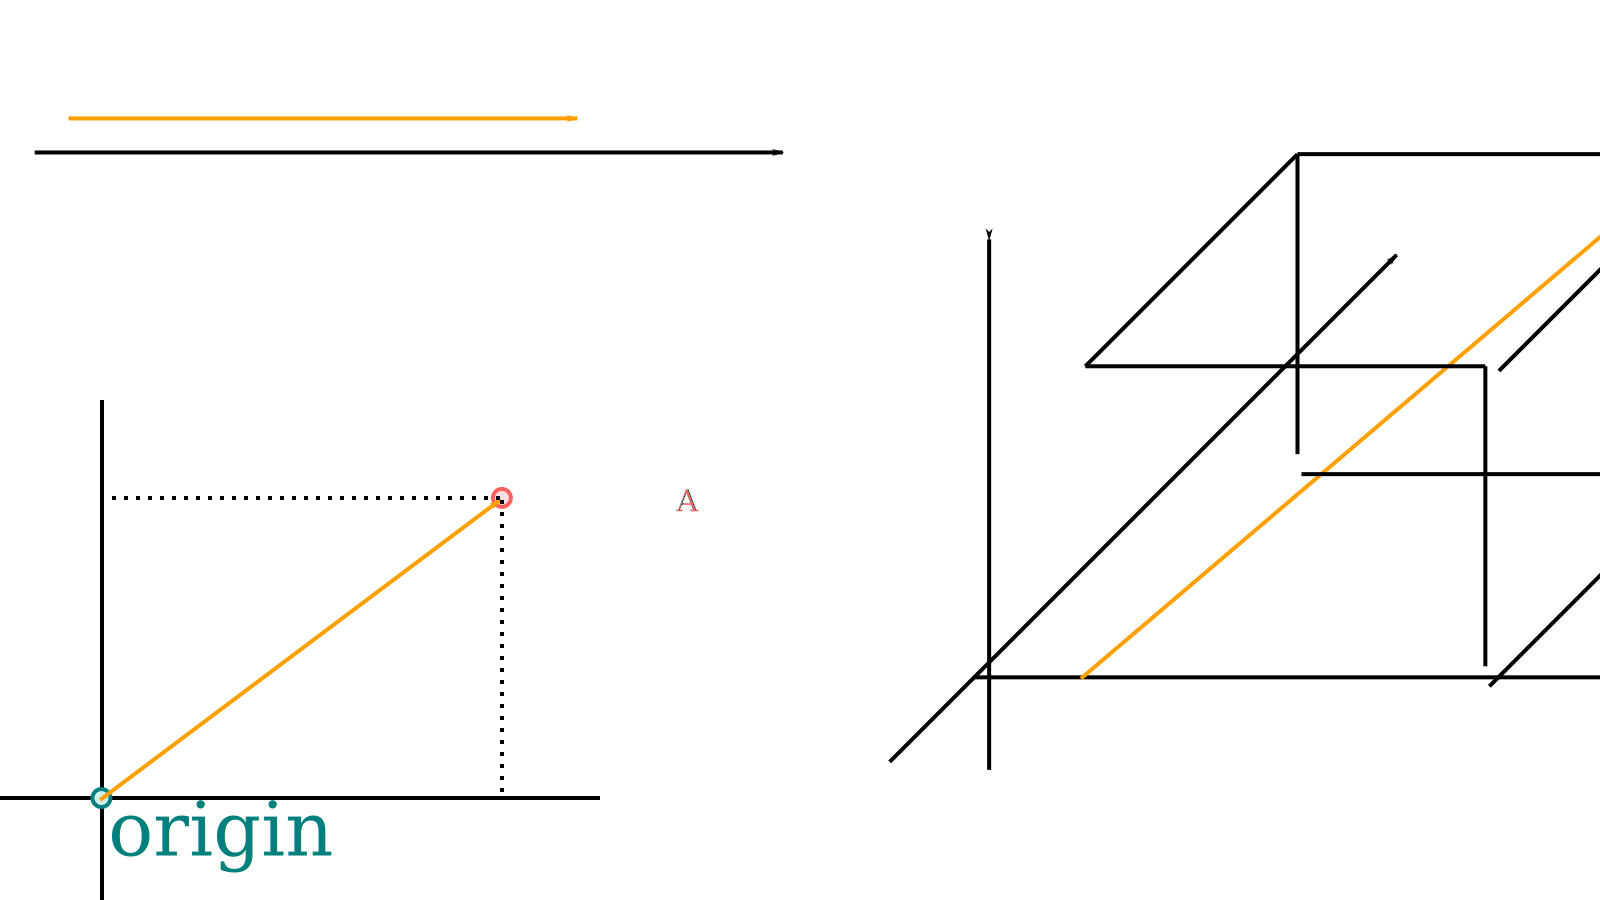
\includegraphics[width=1.0\linewidth]{figures/definePositionVector.png}}
	{\caption[Examples of Position Vector]{Three examples of position vectors shown as arrows in sand color pointed from the origin in teal color to the points in coral color: (a) $\bp_a$ in $\bR{1}$ at coordinate $(4)$ with length 4, (b) $\bp_b$ in $\bR{2}$ at coordinates $(4,\,4)$ with length $4\sqrt{2}$, (c) $\bp_c$ in $\bR{3}$ at coordinates $(4,\,4,\,4)$ with length $4\sqrt{3}$. The origins are located at $(0)$, $(0,\,0)$, and $(0,\,0,\,0)$ respectively.}\label{fig:definePositionVector}}
\end{figure}

%
%
\subsubsection{Subtracting Two Vectors}
\label{ch2sETBssLAsssS2V}
Among the various binary operators with which one could operate on vectors, this thesis is primarily concerned with subtraction, because it will be used to not only calculate the distance between each pair of adjacent points in the mesh, but also in order to interpolate and extrapolate the function values during the calculations of the \wmfv{s} described in detail in Sections~\ref{ch4sIE}~and~\ref{ch4sWM}.

In order to use the subtraction operator on two vectors in the same Euclidean space, one must simply subtract each component element-wise.~\cite{Weisstein19j} For example, given two points in $\bR{3}$, $A$ and $B$, the difference is calculated as
%
\begin{equation}
	A - B = (A_x - B_x,\,A_y - B_y,\,A_z - B_z)
	\label{eq:vectorSubtraction}
\end{equation}
%
which results in the single set of new coordinates, $\{C_x, C_y, C_z\}$, which both represents the point $C$ located there, or the position vector pointed there from the origin.

%
%
\subsubsection{L2-norm}
\label{ch2sETBssLAsssL2N}
The L2-norm may be seen elsewhere in the literature abbreviated as $L^2$ or $\ell^2$, or perhaps called the ``Euclidean norm'' or ``Euclidean distance''. It is so named because it is the ordinary, straight line distance between two points in Euclidean space, and in the case of a position vector $\bP$ in $\bR{3}$, those two points are the origin at $(0, 0, 0)$ and $\bp$ at the coordinates $\{\bP_x,\,\bP_y,\,\bP_y\}$~\cite{Weisstein19h}.

The purpose for calculating the L2-norm of a vector is to determine the ordinary, uni-dimensional length of the vector, regardless of the dimensionality of Euclidean space in which it is embedded. The significance of this distinction can be seen in Figure~\ref{fig:definePositionVector}; despite having all coordinates exclusively set to $4$, the position vector on (a) is of length $4$, in (b) it is of length $4\sqrt{2} \approx 5.657$, and in (c) it is of length $4\sqrt{3} \approx 6.928$.

To determine the length of a vector, one can use the equation for the L2-norm
\begin{equation}
	|\bp| \enspace=\enspace \|\bp\|_2 \enspace=\enspace \sqrt{x^2 + y^2 + z^2 + \ldots + n^2} \enspace:\enspace \bp \in \bR{n}
	\label{eq:l2norm}
\end{equation}

In this thesis, the L2-norm is denoted using the abbreviated symbols $|\bp|$. Please note the similar notation for the cardinality of a set $|\bP|$. While the matching symbols do represent somewhat similar concepts, cardinality is the count of elements in the set, but the L2-norm of a vector is calculated as in Equation~\ref{eq:l2norm}.~\cite[p.~26]{Mara12}
\todoReword{should I just use the long version?}

%
%
%
%
\subsection{Geometry}
\label{ch2sETBssG}
As vast and encompassing is geometry as a field of study, in this section, we will only introduce the few concepts which are of paramount importance for \fors{t}, including: geodesic discs for ensuring a consistent filter widow size for the duration of each convolution in Section~\ref{ch4sSEL}, the characteristics of a circle sector to be used in calculating the area and center of gravity in Section~\ref{ch4sACG}, as well as interpolation and extrapolation for calculating the \wmfv{s} in Section~\ref{ch4sWM}.
\todoResearch{weighted averaging using density}
\todoResearch{static filter window size importance}

%
%
\subsubsection{Geodesic Discs}
\label{ch2sETBssGsssGD}
Geodesy, the term from which geodesic discs get their name, is defined differently in many fields.\todoCitation{geodesy} A geodesic, defined in the original sense, was the shortest route between two points on the Earth's surface; so a straight line distance in curved space. In this thesis, we use the term geodesic disc to mean the surface area on a manifold, encompassed by a circle with a given radius, which itself is also embedded in $\bR{3}$, and reference to such a disc with the symbol $\bO$.
\todoResearch{create figure of geodeisc disc in 3d}

The significance being the similar mathematical treatment of all adjacent faces in any given neighborhood, in order to ensure a consistent filter window size for the duration of each convolution of \fors{t}, despite that given the nature of acquired \tdd{} as discussed in Section~\ref{ch2s3ssAVS3}, which likely all exist on different planes in $\bR{3}$. Also, from the geodesic disc, we derive the circle sectors which are described in detail in the next section.
\todoResearch{static filter window size importance}
\nomenclature[aa]{$\bO$}{a geodesic disc}%
\nomenclature[ab]{$\bO_v$}{a specific geodesic disc centered about the point $\bp_v$}%

%
%
\subsubsection{Circle Sectors}
\label{ch2sETBssGsssCS}
A circular sector, or circle sector, is the portion of a disc enclosed by two radii and an arc. In general, the larger area is known as the major sector, however \fors{t} is only concerned with the area of the other, smaller area, known as the minor sector as it is a natural way to partition a geodesic disc embedded in $\bR{3}$, where each sector can be delineated by the border of two triangular faces which likely exists on different planes.\todoReference{figure of geodesic disc in 3d, once made} Going forward, the minor circle sector will be abbreviated as just ``the circle sector'', or even more simply, ``the sector'', and will be denoted as $\bs$, or $\bs_i$ in reference to a specific circle sector, as described in Section~\ref{ch4sSEL}.%
\nomenclature[ba]{``the sector''}{or the circle sector; the minor sector of a circle defined by its radius and central angle}%
\nomenclature[bb]{$\bs$}{a circle sector}%
\nomenclature[bc]{$\bs_i$}{a specific circle sector}%

As the sector can be described entirely by the central angle $\alpha$ and the circle's radius\footnote{$\ell_{a,b}$ was chosen to represent the radius instead of the much more common $r$, because in \tdd{}, edges are not stored, yet distances between points can be calculated as shown in Section~\ref{ch2s3ssEL}} $\ell_{a,b}$, the area of the sector can be given as
%
\begin{equation}
	A = \pi \ell_{a,b}^2\frac{\alpha}{2\pi} = \frac{\ell_{a,b}^2\alpha}{2}
	\label{eq:areaOfCircleSector}
\end{equation}
%
because of the fact that in radians, the ratio of a sector's central angle $\alpha$ to the complete angle of the circle $2\pi$, is equal to the ratio of that sector's area to area of the whole circle.~\cite{Weisstein19d}%
\nomenclature[bd]{$A$}{an area of a circular sector}%

%
%
\subsubsection{Center of Gravity}
\label{ch2sEBTssGsssCG}
Along with area, the other important characteristic of a circle sector for \fors{t} is the centroid, or center of gravity, which is used in both Algorithms~\ref{alg:serialConvolveFilter}~and~\ref{alg:parallelConvolveFilter} in order to calculate the \wmfv{s}, by serving as the location to which the function values are interpolated, the operation which is discussed in the next section.

The center of gravity is named so, because it is the point where the sector would balance on a pin\footnote{given that it had been bestowed a volume with uniform density}. The center of gravity $\bc$ is calculated as the distance from the center point $\bp_a$, along the line which bisects the central angle $\alpha$, and is given by
%
\begin{equation}
	\check{\ell} := \frac{4\:\gelm\:\sin(\frac{\alpha_i}{2})}{3\,\alpha_i}
	\label{eq:ch2distToCoG}
\end{equation}%%
\nomenclature[ca]{$\bc$}{the center of gravity of circle sector $\bs_i$}%
\nomenclature[cb]{$\check{\ell}$}{the distance from $\bp_0$ to $\bc$}%

In the Figure~\ref{fig:circleSector}, a circle sector is produced by the points $\bp_a$, $\bp_b$, and $\bp_c$, has the central angle $\alpha$, which is bisected by a dotted line, and $\ell_{a,b}$ representing the length between points $\bp_a$ and $\bp_b$, which is equal radius of the circle. Also shown, is the center of gravity $\bc$, as well as $\check{\ell}$, the distance to $\bc$ from the center point $\bp_a$.

\begin{figure}[ht]
\ffigbox
	{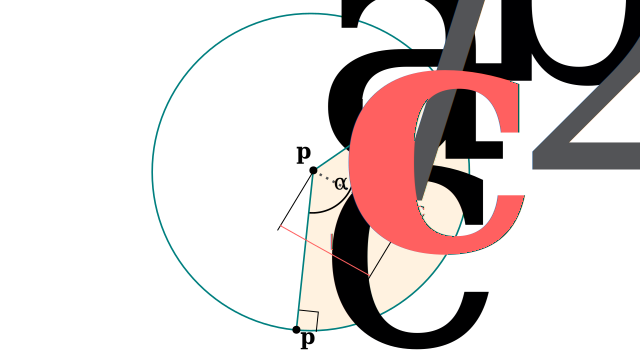
\includegraphics[width=0.6\linewidth]{figures/circleSector.png}}
	{\caption[A Circle Sector in Detail]{The circle sector produced by points $\bp_a$, $\bp_b$, and $\bp_c$, with $\alpha$ as the central angle bisected by a dotted line, and $\ell_{a,b}$ as the length between points $\bp_a$ and $\bp_b$ which is equal radius of the circle. Also labeled is the center of gravity $\bc$ as well as the distance from the center point $\bp_a$ to $\bc$, drawn in a coral color as $\check{\ell}$}\label{fig:circleSector}}
\end{figure}

The line which bisects the central angle of a circle sector, while not used explicitly in calculations, is an important concept for much of the computations used by \fors{t}, as will be seen in Chapter~\ref{ch4}. Therefore, we make a special note here that the abbreviated, ``bisecting line'', indeed refers to this line which splits the circle sector, and its central angle $\alpha$, into two equivalent halves.%
\nomenclature[cc]{``bisecting line''}{the line which bisects the central angle of a circle sector}%

%
%
\subsubsection{Interpolation \& Extrapolation}
\label{ch2sETBssGsssIE}
Simply stated, interpolation is a method of constructing new data points within the range of a discrete set of known data points, such as those points found in the discrete manifolds of in \tdd{}. There exist a large variety of methods for interpolating different kinds of data\todoCitation{different kinds of interpolation}, but in this thesis, we will only consider linear interpolation, which is simple to calculate\footnote{however can become imprecise in relation to the square of the distance between the data points.}\todoCitation{footnote:error of linear interpolation} and can be extended for n-dimensions\todoCitation{n-dimensional linear interpolation}.

Given the two data points in $\bR{2}$, $(x_a, y_a)$ and $(x_b, y_b)$, the $y_c$ coordinate of a third point located along a straight line drawn between the first two points, while also having the coordinate $x_c$, can be calculated as
%
\begin{equation}
	y_c = y_a + (y_b - y_a) \frac{x_c - x_a}{x_b - x_a}
	\label{eq:interpolationGeneral}
\end{equation}

To elaborate the concept of interpolation, now consider the two points $(1, 2)$ and $(5, 1)$, then find the $y$ coordinate of a point between them, located at the intersection of the line which contains the first two points and $x = 3$
%
\begin{align}
	y_c & = 2 + (1 - 2) \frac{3 - 1}{5 - 1} \\
	& = 2 + -1 \frac{2}{4} \enspace = \enspace  1.5
	\label{eq:interpolationSpecific}
\end{align}
%
We therefore interpolate the value halfway between the two given points to be $(3,\,1.5)$, which is halfway between as expected, as illustrated in Figure~\ref{fig:interpolation}.

Conversely, extrapolation is a method for constructing new data points \textit{outside} the range of a discrete set of known data points. The process of linear extrapolation is equivalent\footnote{The difference between interpolation and extrapolation is largely an academic one, owing primarily to the lack of boundaries and increasing error rates associated with extrapolation.} to linear interpolation; namely, first calculating the line between two points, then the $y$ coordinate of a third point at a new value of $x$, either greater than or less than both of the first two points.

As illustrated by Figure~\ref{fig:interpolation}, the similarities and differences between the processes of interpolation and extrapolation, become even more intuitive when seen graphically, where having chosen the two points $\bp_a$ and $\bp_b$, a third point $\bp_c$ is interpolated between the two points, while the fourth point $\bp_d$ is extrapolated outside their domain.

\begin{figure}[ht]
\ffigbox
	{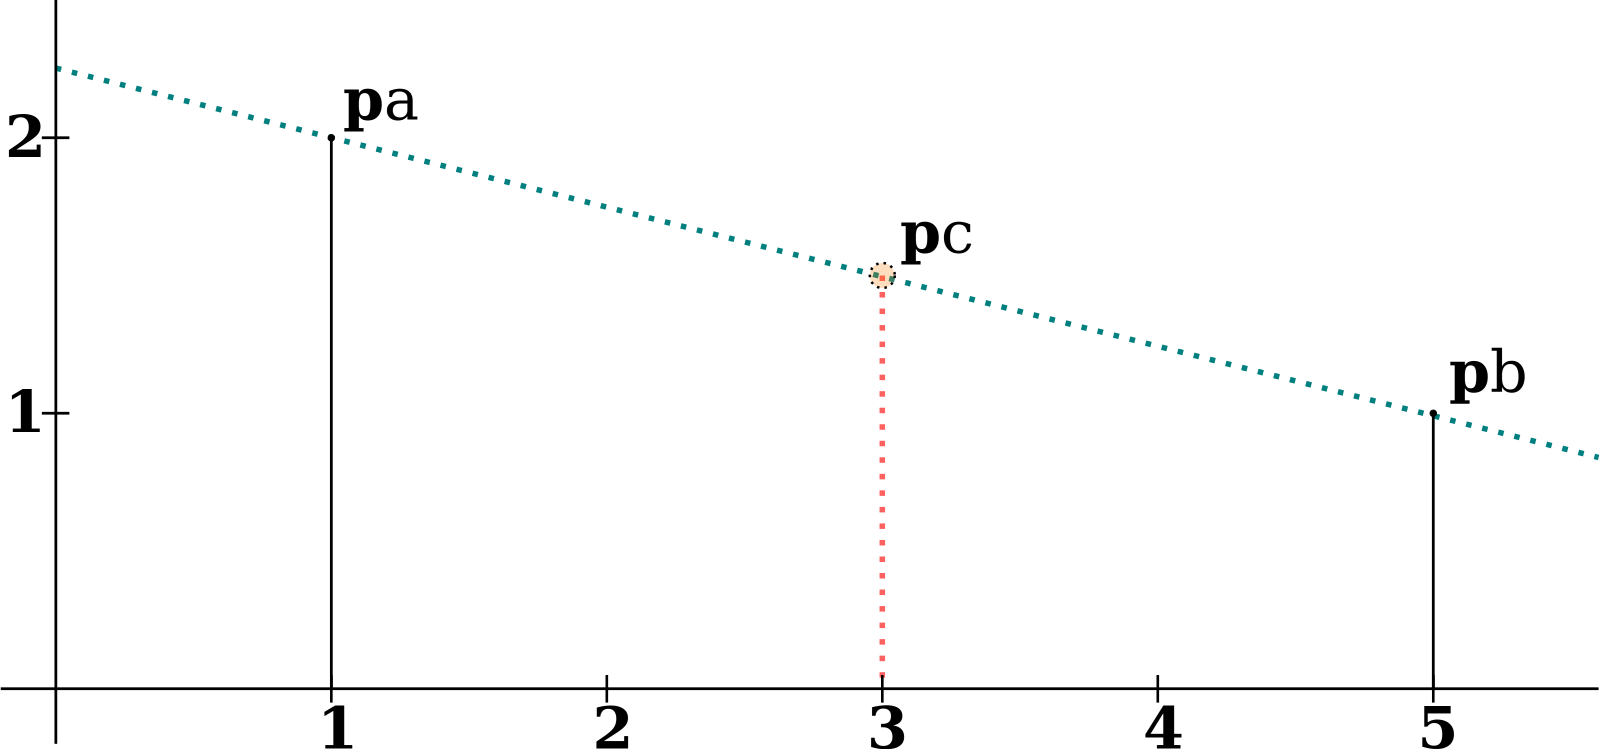
\includegraphics[width=1.0\linewidth]{figures/interpolation.png}}
	{\caption[Interpolation between two points in $\bR{2}$]{$\bp_c$ is interpolated as a value between $\bp_a$ and $\bp_b$}\label{fig:interpolation}}
\end{figure}

Later in this thesis, we will use both interpolation and extrapolation together, in order to calculate the \wmfv{s} at the center of gravity of circle sectors, so that the function values may be weighted fairly in regards to their distance to the other points in the one-ring neighborhood, as discussed in detail in Section~\ref{ch4sIE}.

%
%
%
%
\subsection{Topology}
\label{ch2sETBssT}
Topology is the mathematical study of the properties of space that are preserved through deformations, twistings, and stretchings of objects\footnote{but not tearing or gluing}, which developed as a field of study from geometry and set theory through analysis of concepts such as space, dimension, and transformation. For example, a circle is topologically equivalent to an ellipse, because it can be deformed by stretching.~\cite{Weisstein19c}

Of all the major concepts studied in topology, this thesis is only concerned manifolds, as \tdd{} is composed primarily of two-dimensional discrete manifolds embedded in three-dimensional space, as well as neighborhoods, the general concept from which one-ring neighborhoods are derived, thus the basis upon which \fors{t} is founded.

%
%
\subsubsection{Manifolds}
\label{ch2sETBssTsssM}
A manifold is a topological space that is locally, but possibly not globally, Euclidean; a concept that is central to many parts of geometry because it allows complicated structures, such as the triangle mesh, to be described and understood in terms of the simpler, local topological properties. Said another way, this means that a manifold is an $n$D-subset of an Euclidean space $\mathbb{R}^{>n}$.~\cite[p.~199]{Mara12} For example, 1-dimensional manifolds in $\mathbb{R}^{2}$ include lines and circles, and 2-dimensional manifolds in $\mathbb{R}^{3}$, also called surfaces, can include commonly-known shapes such as the plane, the sphere, and the torus, but also of prime importance for this thesis, the triangle mesh.

The significance to our research, is that each convolution of \Fors{t} is comprised of calculations of the \wmfv{s} at the central point of a one-ring neighborhood, having weighted the function values in relation to the distance between each neighbor, and because those distances are uniformly dissimilar in acquired \tdd{}\todoCitation{tdd{} is not regular}, maintaining a consistent filter window size is only accomplished by defining the geodesic disc, which exists on the manifold defined by the mesh. Therefore, as discussed in more detail in Chapter~\ref{ch4}, the weights may be calculated sector-wise, as if all sectors were on the same plane, greatly reducing the complexity of the entire procedure.

%
%
\subsubsection{Neighborhoods}
\label{ch2sETBssTsssN}
A neighborhood is also one of the basic concepts of topology. Intuitively speaking, a neighborhood of a point is a set of points containing that point, where one can move in any direction without leaving the set. While determining the neighborhood is trivial for uni-dimensional manifolds\footnote{where each neighborhood only consists of a point, and the two points to either side of it on the line}, and relatively simple for regular two-dimensional manifolds\footnote{such as with a 2D-image, whose pixels have at most four neighbors in orthogonal directions with a geometric distance of 1, as well as four neighbors at the diagonal directions with a geometric distance of $\sqrt{2}$}, determining the neighborhood becomes more complicated for irregular surfaces like those found in \tdd{}. With those surfaces, one must determine the set of neighbors using the associations that define the triangular faces; the details of which are covered in detail in Section:~\ref{ch2s3ssORN}, after the necessary topics regarding \tdd{} have already been discussed.

Figure~\ref{fig:neighborhoods} illustrates the differences among one-ring neighborhoods in different kinds of manifolds: (a) a regular square mesh as with pixels of a digital image, (b) a regular triangle mesh, as in a hexagonal tessellation, then in (c) the figure shows two very different neighborhoods in a single, irregular triangle mesh typical of acquired \tdd{}. In particular, notice in (c) the completely arbitrary shape and size of the one-ring neighborhoods found in the irregular triangle mesh; even the number of neighbors varies widely. From this observation is where much of the motivation behind \fors{t} came.

\begin{figure}[ht]
\ffigbox
	{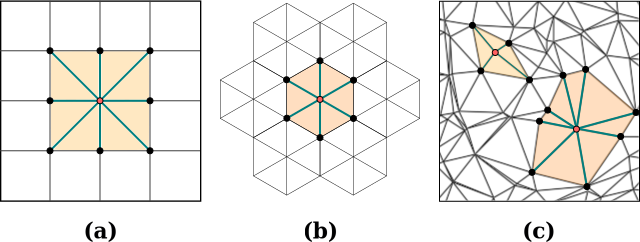
\includegraphics[width=1.0\linewidth]{figures/neighborhoods.png}}
	{\caption[One-ring neighborhoods in regular and irregular meshes]{One-ring neighborhoods in (a) a regular square mesh, as in pixels of a digital image (b) a regular triangle mesh, as in a hexagonal tessellation (c) an irregular triangle mesh, typical of acquired \tdd{}}\label{fig:neighborhoods}}
\end{figure}

%
%
%
%
%
%
\section{\tdd}
\label{ch2s3}
The data upon which one convolves \fors{t} is called \tdd\todoCitation{\tdd{} name origin, BB82 from Mara12}. As described in Section~\ref{ch2s3ssM}, \tdd{} consists primarily of a single mesh $\bM$, which is composed of $\bP$, a set of points, and the set $\bT$, consisting of triangular faces, each to be covered in Sections~\ref{ch2s3ssP} and~\ref{ch2s3ssF} respectively. \tdd{} also comes in two distinct flavors depending on its origin: acquired or synthetic, as discussed in Section~\ref{ch2s3ssAVS3}. The data can also include a texture map and other various types of information stored as scalar or vector fields, as elaborated on in~\ref{ch2s3ssFV}.

%
%
%
%
\subsection{Points}
\label{ch2s3ssP}
A point $\bp$ is the most primitive element of \tdd{}. ``Point'' is the abbreviated form of ``measuring point'', and is also known in other fields of study as a vertex, or a position vector $\bR{3}$\todoCitation{other names for a point}. A point is defined by the 3-dimensional Cartesian coordinates $x$, $y$, and $z$, and in \tdd{}, points are generally unique and not required to be in any particular order. In this thesis, a point is addressed using several different subscripts, depending on the context.

In this thesis, when referring to a point in $\bP$, $v$ is used as the globally unique index; the index with which we can define the set
%
\begin{equation}
	\bP := \left \{\:\bp_v \mid v \in \mathbb{N}, \;\text{and}\; 1\leq v \leq v_{max}\:\right \}
	\label{eq:defineSetOfPoints}
\end{equation}
%
where $v_{max}$ is the maximum index\footnote{\label{indicesFootnote}Beginning indices with 1 is significant because of the discordant conventions between addressing the first element of a data structure with 0 in programming languages, such as C++ and python, versus addressing first elements with 1, as is the standard for mathematical literature. Because this thesis should indeed be considered mathematical literature, we will always start indices at 1, and only use index 0 for special cases. For example, $\bp_0$ is used in Chapter~\ref{ch4} to represent the center point of the one-ring neighborhood.} of points in the data, and is equivalent to the cardinality of the set of points $|\bP|$.%
\nomenclature[ea]{$\bP$}{the set of points $\bp$ in $\bM$}%
\nomenclature[eb]{$\bp_v$}{a specific point in $\bP$}%

Otherwise, when referencing to a point within a particular face or neighborhood, the three corners can be referenced indirectly\footnote{or even more generally, as $\bp_a$, $\bp_b$, and $\bp_c$ in the case of Equation~\ref{eq:defineEdgeLengthFace}, or in the case of a nested loops: as $\bp_j$ and $\bp_{\sjpo}$ in Algorithms~\ref{alg:serialConvolveFilter}~and~\ref{alg:parallelConvolveFilter}} as $\bp_i$, $\bp_{\sipo}$, and $\bp_{\sipt}$, or directly as $\bp_0$\footref{indicesFootnote}, $\bp_1$, $\bp_2$, etcetera.~\cite[p.~25]{Mara12}%
\nomenclature[ec]{$\bp_i$}{also $\bp_{\sipo}$, and $\bp_{\sipt}$; one of three indirectly referenced points comprising a face}%

%
%
%
%
\subsection{Faces}
\label{ch2s3ssF}
Faces are the another primitive element of \tdd{}. As we are working exclusively with triangular meshes~\cite[p.~26]{Mara12}, we define a face $\bt$ by the set of three distinct points, which we will index in clockwise order\footnote{It is worth mentioning here that many software packages, such as the GigaMesh Framework~\cite[p.~89]{Mara12}, may expect counter-clockwise ordering of indexes. This is significant because the ordering provides an orientation by which visualization software can apply texture and/or lighting. The only mathematical significance of the ordering is the sign of the area of a face, and totally inconsequential when the absolute value is expected, as shown by~\cite[p.~2]{Braden86}. This is yet another example of the difference between the conventions of mathematical literature versus those of computer science. And again, because this thesis should indeed be considered mathematical literature, we will continue to follow the conventions of mathematical literature.}~\cite[p.~4]{Mara17}.
\todoResearch{does the "right-hand-rule apply here?"}
%
\begin{equation}
	\bt := \left \{\,\bp_a,\,\bp_b,\,\bp_c\right \} = \left \{\,\bp_1,\,\bp_2,\,\bp_3\right \}
	\label{eq:defineFaces}
\end{equation}

With the introduction of faces comes the concept of adjacency. A face $\bt_i$ is said to be adjacent to another face $\bt_j$ if, and only if, they share together the same subset of two points. Similarly, a point $\bp_a$ is said to be adjacent to another point $\bp_b$ if, and only if, the set $\{\bp_a, \bp_b\}$ is a subset of at least one face $\bt \in \bT$. A synonym for adjacent is ``neighboring'', and this thesis will use both interchangeably. \todoReword{add equation for these identities}\todoReword{index entry for adjacent}

Figure~\ref{fig:triangularFaces} shows two adjacent triangular faces $\bt_1$ and $\bt_2$, and the relationship between their points $\bp_a$, $\bp_b$, and $\bp_c$, their edge lengths $\ell_a$, $\ell_b$, and $\ell_c$, and their clockwise orientation. Because the concept illustrated in this figure is fundamental to understanding the structure of all \tdd{}, therefore also \Fors{t}, and yet may not be immediately intuitive without proper context, we reference this figure several times throughout the rest of this thesis.

\begin{figure}[ht]
\ffigbox
	{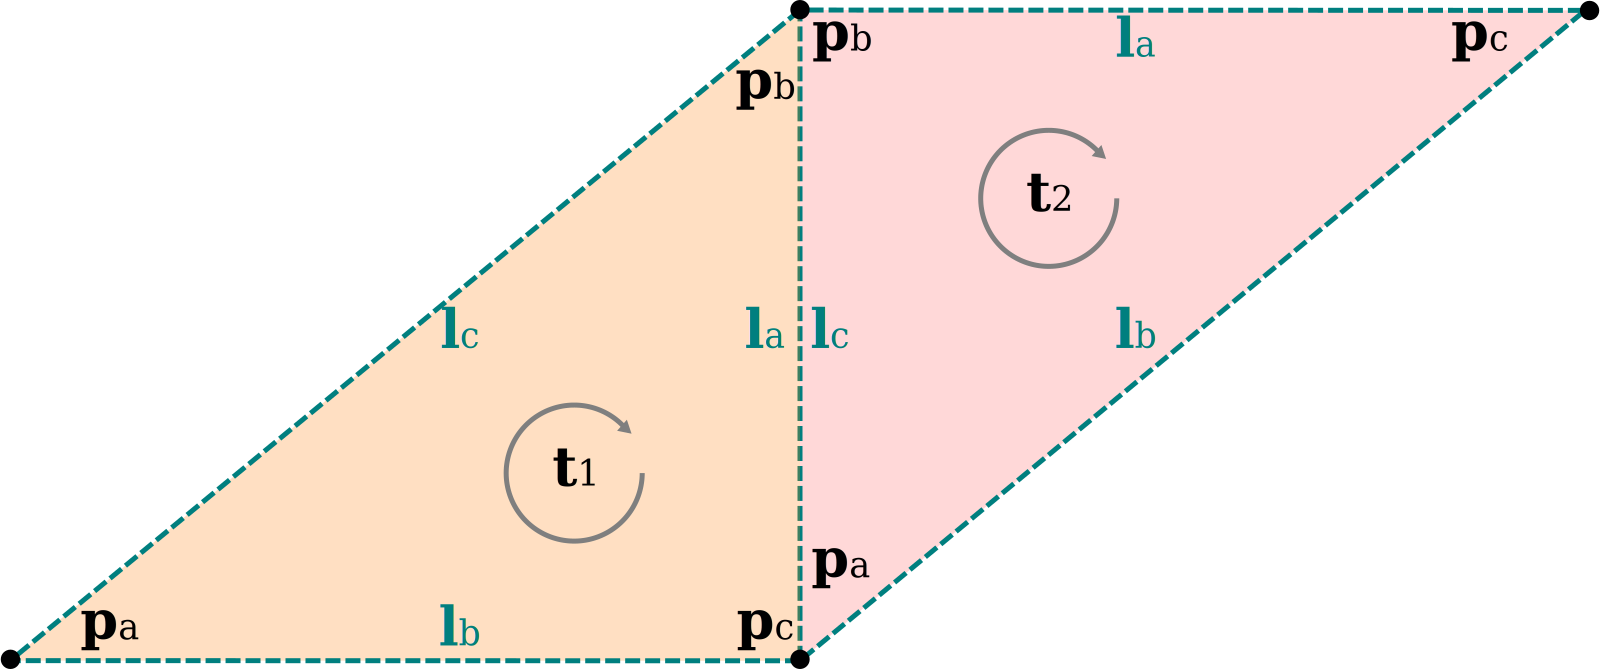
\includegraphics[width=1.0\linewidth]{figures/triangularFaces.png}}
	{\caption[Two Triangular Faces]{Two adjacent triangular faces $\bt_1$ and $\bt_2$, showing the relationship between their points $\bp_a$, $\bp_b$, and $\bp_c$, their edge lengths $\ell_a$, $\ell_b$, and $\ell_c$, and their clockwise orientation.}\label{fig:triangularFaces}}
\end{figure}

Each distinct triangular face is addressed using the global index $k$, and when taken together, comprise the set
%
\begin{equation}
	\bT := \left \{\:\bt_k \mid k \in \mathbb{N}, \;\text{and}\; 1\leq k \leq k_{max}\:\right \}
	\label{eq:defineSetOfFaces}
\end{equation}
%
where $k_{max}$ is the maximum index of faces in the data, and is equivalent to the cardinality of the set of faces $|\bT|$.%
\nomenclature[fa]{$\bT$}{the set of faces $\bt$ in $\bM$}%
\nomenclature[fb]{$\bt_k$}{a specific face in $\bT$}%

%
%
%
%
\subsection{Edge Lengths}
\label{ch2s3ssEL}
As illustrated in Figure~\ref{fig:triangularFaces}, each triangular face is implicitly composed of three edges. Despite the fact that an edge is not typically\footnote{Other data structures, such as the Winged-Edge~\cite[p.~1]{Baumgart75}, may use edges as a primitive element} a primitive element of \tdd{}, we will endeavor to define the length of an edge $\ell$, because edge lengths are of particular significance for both the design and implementation of \fors{t}.

What is also particularly interesting about Figure~\ref{fig:triangularFaces}, is that when edge lengths are defined by the points of specific faces, each non-border edge length, illustrated in the figure as $\ell_a$ in $\bt_1$, and $\ell_c$ in $\bt_2$, will be labeled twice, despite representing the same distance.

When in the context of a particular face $\bt_k$, we will use a single index to define the length
%
\begin{equation}
	\ell_a := |\bp_b - \bp_c| \enspace:\enspace \left \{\,\bp_a,\,\bp_b,\,\bp_c\right \} = \bt_k
	\label{eq:defineEdgeLengthFace}
\end{equation}%
\nomenclature[ga]{$\ell_i$}{the length of the edge opposite the point $\bp_i$ of a specific face}%
%
and double indices when an edge length is referenced in relation to a specific point $\bp_v$ and its neighbor $\bp_i$
%
\begin{equation}
	\ell_{\sv{i}} := |\bp_i - \bp_v|
	\label{eq:defineEdgeLengthPoint}
\end{equation}%
\nomenclature[gb]{$\ell_{\sv{i}}$}{the length of the edge between points $\bp_v$ and $\bp_i$}%

Please note the similar notation for the cardinality of a set $|\bP|$, to that for the calculation for the length of the edge $|\bp_i - \bp_v|$ as defined in Equation~\ref{eq:defineEdgeLengthPoint}. While cardinality is simply the count of elements in the set, the length is calculated as the L2-norm of the referenced vector.~\cite[p.~26]{Mara12}

\begin{equation}
\begin{aligned}
	|\bp_i - \bp_v| & = \lVert\bp_i - \bp_v\rVert_2 \\
					& = \sqrt{(x_i-x_v)^2 + (y_i-y_v)^2 + (y_i-y_v)^2}
	\label{eq:defineEdgeLengthCalc}
\end{aligned}
\end{equation}
\todoResearch{can I avoid sqrt altogether by performing entire algorithm squared?}

%
%
%
%
\subsection{Meshes}
\label{ch2s3ssM}
In \tdd{}, a mesh $\bM$ is the digital representation of a discrete manifold embedded in $\bR{3}$, and is typically\footnote{except in the case of specifically designed synthetic data~\ref{ch7sSD}} two-dimensional, non-planar and comprised of non-regular, triangular faces composed of connected points.~\cite[p.~25]{Mara12} A mesh is the set defined as
%
\begin{equation}
	\bM := \left \{\bP,\:\bT\right \}
	\label{eq:defineMesh}
\end{equation}%
\nomenclature[da]{$\bM$}{a mesh; the set including the sets of all points $\bp$ and faces $\bt$}%
%
with the set $\bP$ consisting of points, and the set $\bT$ consisting of triangular faces.

Many 3D-scanners produce point clouds\todoCitation{3D-scanners produce point clouds}, which as the name suggests, are comprised soley of a set of points $\bP$ and do not provide the set $\bT$. However, it is possible, and necessary for the production of a mesh, to perform a point set triangulation\todoCitation{perform a point set triangulation} in order to connect $\bP$ into a set of triangle faces, enabling one to combine the two sets into a mesh.~\cite[p.~26]{Mara12} For example, during our experiments, we perform the well-known Delaunay triangulation\todoCitation{Delaunay triangulation} in order to produce a mesh from a randomly generated point cloud\todoReference{experiments}.
\todoResearch{add figure of point cloud to triangulation}

%
%
%
%
\subsection{One-Ring Neighborhoods}
\label{ch2s3ssORN}
It was mentioned in Section~\ref{ch2sETBssTsssN}, that it is a non-trivial task to determine the neighborhood of a point $\bp_v$, which exists in an irregular triangle mesh embedded in three-dimensions. Having now examined the definitions of points, faces, and meshes, we can now formalize the one-ring neighborhood in \tdd{} as
%
\begin{equation}
	\bN_v := \left \{\;\bp_i\;:\;\left \{\,\bp_i,\,\bp_v\right \} \subseteq \bt \quad \forall \bt \in \bT\;\right \}
	\label{eq:defineNeighborhood}
\end{equation}%
\nomenclature[ha]{$\bN_v$}{the set of points comprising the one-ring neighborhood about $\bP_v$}%
\nomenclature[hb]{$\bp_i$}{a one-ring neighbor of $\bp_v$}%
%
which in words, means that the neighborhood $\bN_v$ is defined as the set of points $\bp_i$ such that both $\bp_i$ and $\bp_v$ are two points of a triangular face $\bt$, for all faces in the mesh. Therefore, the adjacency of points is defined by the co-membership within a face $\bt$, from the set of faces $\bT$.

When taken together, all the neighborhoods $\bN_v$ comprise a set of sets of neighbors; the family of sets
%
\begin{equation}
	\bN := \left \{\bN_v,\,\bN_{v+1},\ldots,\,\bN_{v_max}\right \}
	\label{eq:defineNeighborhood}
\end{equation}%
\nomenclature[hc]{$\bN$}{a family of sets of neighbors, the set of neighborhoods}%
This definition shares the indices $v$ and $v_{max}$ with the definition for a set of points, Equation~\ref{eq:defineSetOfPoints}, to highlight the fact that neighborhoods are defined per point, therefore there must be a correlation in the cardinality between the two sets.

Conversely, the cardinality of each individual neighborhood $|\bN_v|$ will likely vary among other neighborhoods in $\bN$, however, the value must always be $\geq 2$, and though there is no upper limit, $|\bN_v|$ is typically $\leq 12$. Furthermore, the neighboring points are always indexed in a clockwise direction for the same reasons as discussed in Section~\ref{ch2s3ssF}.
\todoResearch{get real upper limit for n}.%

As illustrated in Figure~\ref{fig:neighborhoods}, the set of black points are the neighbors $\bp_i$ which belong to $\bN_v$, what is known as a one-ring neighborhood\footnotemark of $\bp_v$, because they are directly connected with the center point $\bp_v$ drawn in coral color. The moniker originates from graph theory where each adjacent point is said to have a relative distance of 1 within the graph of the mesh. \footnotetext{The one-ring can be extended to a 2-ring by taking the union of the neighborhood $\bN_v$ with the neighborhood of each one-ring neighbor $\bp_i$, which adds to the neighborhood, points with the relative distance of 2 within the graph. This iterative concept can be repeated k times and the neighborhood is than referred to as k-ring. Unfortunately, regardless of the fact that the relative distance within the graph can not be assumed equal to the geometric distance nor geodesic distance, it is still used throughout the literature – especially in the field of Computer Graphics.~\cite[p.~29]{Mara12}}
\todoBackground{add a subsection on graph theory in basic theory section}

Our solution for maintaining a constant filter window size while convolving \fors{t} over neighborhoods of varying shapes and sizes is to determine the global minimum edge length, then use that as the radius of the geodesic disc centered at the central point of a neighborhood, in order calculate the \wmfv{s} of each circle sector, after interpolating each value function value from the neighboring points to the center of gravity, as explained in greater detail in Chapter~\ref{ch4}, later in this thesis.

%
%
%
%
\subsection{Acquired vs Synthetic \tdd{}}
\label{ch2s3ssAVS3}
The corpus of all \tdd{} exists in two flavors, acquired and synthetic data, with each being handily classifiable by the fashion in which it was generated, and the characteristics innate to those techniques.\todoReword{consider adding a figure here showing difference, or referencing a figure or pair of figures that does}

Acquired \tdd{} is typically captured as a point cloud utilizing various methods, such as: LiDAR (Light Detection and Ranging), Structured Light, or Structure from Motion~\cite[p.~19]{Mara12}. Then the data is exported from software packages accompanying the 3D-scanners as either just the point cloud as a simple set of points $\bP$, or optionally as a triangle mesh $\bM$, described by one or more scalar-fields. Acquired \tdd{} also often consists upwards of a million points and as many as twice that number of faces\todoReference{the interesting experimental finding about face to vertex ratio; add as a footnote}. These exported meshes ~\cite[p.~25]{Mara12} uniformly contain noise and may exhibit other complexities for analysis, such as: non-manifold points, multiple borders and holes in the surface, inverted face orientation, non-manifold edges, and agglutination or degenerate faces. ~\cite[p.~28-32]{Mara12}

Conversely, synthetic \tdd{} is artfully crafted to avoid the complexities exhibited by acquired data. When modeling 3-dimensional objects, synthetic \tdd{} can require significantly less memory for storage, as simplifications can be made for large regular surfaces. For example, even the largest flat, rectangular surface can be modeled with only four points and two faces, whereas the acquired data methods require that the Nyquist–Shannon sampling theorem\todoCitation{Nyquist Shannon Theorem} be obeyed for the smallest detectable feature throughout the entire surface.~\cite[p.~19]{Mara12}~\cite[p.~3]{Mara17}

For our experiments\todoReference{experiments}, we created another kind of synthetic \tdd{} which does not model a 3D-object. Instead, these synthetic-mesh generators produce different types of tessellations on arbitrarily large, planar surfaces, accompanied by a configurable scalar-field of function values.

%
%
%
\subsection{Function Values}
\label{ch2s3ssFV}
In addition to the three Cartesian coordinates, point which comprise a mesh may also contain other relevant data in the form of scalar fields, or vector fields, when combined together into multi-dimensional data. This information, which is stored at each point $\bp$, often includes data regarding: RGB color, material type, reflectivity, transparency, quality, confidence, or the resulting function values from an analytical filter such as the Multi-Scale Integral Invariants (MSII) filter~\cite[p.~21]{Mara12}, but can be extended to include data important to other fields of study, such as: infrared or ultraviolet light, temperature, rainfall, population, crime-rates, etc; essentially, any kind of data that may be measured at a point. As \fors{t} will currently\todoReference{future work/applications} only process a single field at a time, we can define a scalar field simply as the set of function values
%
\begin{equation}
	\bF := \left \{\: f_v \mid v \in \mathbb{N}, \;\text{and}\; 1\leq v \leq v_{max} \:\right \}
	\label{eq:defineSetOfFunctionValues}
\end{equation}%
\nomenclature[ia]{$\bF$}{the set of function values $f$; a scalar field}%
\nomenclature[ib]{$f_v$}{a specific function value in $\bF$, corresponding to $\bp_v$}%
%
This definition shares the indices $v$ and $v_{max}$ with, Equation~\ref{eq:defineSetOfPoints}, the definition for a set of points, because indeed, it is a fact that the cardinality of $|\bF|$ must be equal to $|\bP|$
%
\begin{equation}
	|\bF| \mbeq |\bP|
\end{equation}
%
because function values are only stored alongside the Cartesian coordinates, 1-for-1 with points, due to \tdd{} existing as a discrete manifold. The significance of which is another motivating factor behind the research conducted in this thesis.

%
%
%
%
%
%
\section{Parallel Processing}
\label{ch2sPP}

%
%
%
%
\subsection{Architecture of Concurrency} %Hardware
Of the 4 classifications of the architectures of concurrency\todoCitation{Flynn, 1966 doi:10.1109/TC.1972.5009071.}, this thesis is primarily concerned with SIMD\footnote{or SIMT as is branded by NVIDIA}\todoCitation{NVIDIA SIMT 4.1. SIMT Architecture}, single instruction, multiple data streams, which is the architecture of commercial workstations in use today. The SIMD classification is characterized by single instructions being executed in parallel on multiple data, which means simultaneously, typically requiring synchronization before the results may be further processed.

Figure~\ref{fig:simdArchitecture}, illustrates a simplified impression of system which employs SIMD architecture.

\begin{figure}[ht]
\ffigbox
	{\includegraphics[width=1.0\linewidth]{figures/simdArchitecture.png}}
	{\caption[SIMD Architecture]{The architecture characterized as SIMD by Flynn's Taxonomy of systems, where a single instruction is executed simultaneously, in parallel, on }\label{fig:simdArchitecture}}
\end{figure}\todoCitation{Flynn, 1966 doi:10.1109/TC.1972.5009071.}

The major advantage obtained by implementing software in SIMD system is the speedup gained when repetitive tasks which would otherwise be executed serially in a loop, one after another, can instead be computed simultaneously, incurring only minor synchronization overhead. Any operation performed in linear algebra, such as the multiplication of an entire vector by a scalar, is thus made much more scalable in regards to the time required to complete the computation for growing sizes of vectors.

This concept can be extended to more complex programs, and indeed, the topic of the research presented in this thesis is implementing the convolutions of the complex algorithm for \Fors{t} to be executed for every point in a mesh, simultaneously, in parallel, on a SIMD system.

All modern computers implement some form of parallelism, be it multi-core or multi-threaded processors, stream processors as found in GPUs, or networks of supercomputers or data centers. This thesis will focus on implementing \fors{t} in a way which can utilize the parallelism provided by the array of stream processors found in a commercially available GPGPU.

GPGPU stands fo General Use Graphics Processing unit, as coined by Mark Harris, the founder of GPGPU.org\todoCitation{Mark Harris}, coined the term GPGPU.and it describes the hardware

The technology

%\subsection{Host Memory and Device Memory}
\todoBackground{memory vs speed}
Hardware consists of memory and processors. Memory is divided into a hierarchy which starting at the registers on the processors themselves, increases in capacity, but decreases in speed.\todoReword{moves away from} Of particular interest to this thesis...\todoReword{continue}



%
%
%
%
\subsection{Serial Computation \& Threads}
\todoBackground{"spawning a thread"}
In a very general sense, when a computer executes a serial program, it proceeds one instruction at a time, sequentially in the order that it is written, reading and writing to memory as required. Individually, these are called threads of execution, and a single processing core can only process a single such thread at a time, however, it can rapidly perform context switching\todoCitation{context switching} among a multitude of self-contained threads, each with their own unique ids and memory addresses, in order to give the illusion of parallel processing.

As memory to be processed by a thread is stored somewhere in a hierarchy which increases in size, but decreases in speed as one moves from the processor's registers, it is likely that a context switch will cause what is known as a cache miss\todoCitation{cache hit or miss, check Lang}, which incurs a time penalty while the processing stalls and the required memory is read from slower hardware sources.



%
%
%
%
\subsection{Program Correctness}
\ldots

%
%
\subsubsection{Control \& Data Dependencies}
\label{ch2sPPssCS}
%Data Dependencies: ~\cite[p.~358]{Lang17}
%Section~\ref{ch2sACssCVP}
%Data Partitioning:
%Calculations depend on specific data structures.~\cite[p.~357]{Lang17}
%As in edge lengths depend on the neighborhoods.
\todoResearch{https://en.wikipedia.org/wiki/Loop-level\_parallelism}
%True (Flow) Dependence	S1 ->T S2	A true dependence between S1 and S2 means that S1 writes to a location later read from by S2
%Anti Dependence	S1 ->A S2	An anti-dependence between S1 and S2 means that S1 reads from a location later written to by S2.
%Output Dependence	S1 ->O S2	An output dependence between S1 and S2 means that S1 and S2 write to the same location.
%Input Dependence	S1 ->I S2	An input dependence between S1 and S2 means that S1 and S2 read from the same location.
The concepts of control and data dependencies are not new ones, and can be dated back to the invention of multi-pass compilers\todoCitation{Data Dependencies and multi-pass compilers}. The field of study regarding the details is called dependence analysis and has far-reaching consequences from business management, economics, as well as software optimization\todoCitation{dependence analysis}. In general, the basic concept behind both control and data dependencies is that some procedure A is said to be dependent on another procedure B, if A requires B to be executed first.

Figure~\ref{fig:simpleControlDependency} shows the ubiquitous if-then control structure as a simple example of a control dependency. It reads, ``if B is true, then do A''. In this case A is control dependent on B, because B must execute before it can be determined wether or not to execute A.

\begin{figure}[ht]
	\includestandalone[width=0.35\textwidth]{figures/tikz/simpleControlDependency}
	{\caption[If-Then Control Dependency]{A simple example of control dependency using the if-then control structure, with each distinct operation colored in teal, and control dependency marked with an arrow.}\label{fig:simpleControlDependency}}
\end{figure}

Figure~\ref{fig:dataDependencyOfL2Norm} illustrates the less-than-simple example of data dependencies inherent to calculating the L2-norm of a position vector in $\mathbb{R}^{3}$, which has already been seen in Equation~\ref{eq:l2norm}, and will be seen often in this thesis. There are six individual procedures involved with calculating the L2-norm: three squarings, two additions, and one square root. The three squaring procedures are totally independent of each other and can be performed in any order, indeed even concurrently, in relation to one another. In contrast, the two additions are totally dependent on their addends. While the order in which the first two of the three addends are used is inconsequential, the first addition is always dependent on the completion of two squarings, and the second addition is dependent on not only the sum from the first addition, but the product of the third squaring as well. Finally, because the square root procedure is dependent on the execution of both additions, it also inherits their dependencies on the squaring procedures, and therefore must wait until the very end before executing last.\todoResearch{name of this inheritance, associative?}

\begin{figure}[ht]
	\includestandalone[width=1.0\textwidth]{figures/tikz/dataDependencyOfL2Norm}
	{\caption[Data Dependencies in the L2-norm Calculation]{The data dependencies inherent to calculation of the L2-norm of a position vector in $\bR{3}$, with each distinct operation colored in teal, and data dependencies marked with arrows. The centered block in sand color represents an exclusive-or situation, abbreviated as xor, where one, and only one pair of operations shall execute.}\label{fig:dataDependencyOfL2Norm}}
\end{figure}

%
%
\subsubsection{Critical Sections}

%
%
\subsubsection{Mutexes}
%Mutexes and semaphores (binary semaphore}
While it is true that any locking mechanism can be expensive to both compute time and memory, \todoResearch{how expensive are locking mechanisms} typically, with acquired \tdd{}, the ratio of points in $\bP$ to the average neighborhood size \todoReword{add symbol for average neighborhood size} approaches $|\bP|$, therefore the speedup gained by exploiting the concurrency is definitely\todoResearch{quantify the cost} worth the cost of the added synchronization overhead when computing with even moderately sized meshes on a SIMP or SIMT modeled architecture.
starts at ~\cite[~p.20]{Lang17}

%
%
\subsubsection{Explicit Synchronization}%3.2.5.5.3. Explicit Synchronization}
\todoBackground{synchronizeThreads()}
sand color to highlight the fact that the values stored in memory will change throughout the life of the total procedure, and without the protection of a locking mechanism, therefore, extra care must be taken so that the implementation of the parallel variant of the serial algorithm will maintain correctness.

%
%
%
%
\subsection{Evaluation and Analysis of Concurrent Algorithms}~\cite[p.~330]{Lang17}
\subsubsection{Timing}
\begin{equation}
	N = input size (num. ops)
	P = processor count
	Ts(N) = Sequential execution time
	Tbest(N) = Optimal execution time
	TP(N, P) = Parallel runtime
\end{equation}
\subsubsection{Speedup, efficiency}
	Speedup:
S(N, P) = Tbest(N)/TP(N, P)

	Efficiency:
E(N, P) = Tbest (N)/PTP(N, P) = S/P

	Costs:
C(N, P) = PTP(N, P)

\subsubsection{Degree of Parallelism}
	0 < q < 1 is the sequential part
	1-q = is the parallelizable part


%\subsection{Hardware Implementation}%4. Hardware Implementation}
%\section{CUDA extended C++: An interface for GPGPU implementation}
%\subsection{CUDA C Runtime}%3.2. CUDA C Runtime}
%\subsection{Versioning and Compatibility}%3.3. Versioning and Compatibility}
%\subsection{Versions <9, vs >= 9}
%
%\subsection{Iso-efficiency}
%	WK(P) = iso-efficient if it fulfills:
%	TO(WK(P), P) = KWK(P)~\cite[p.~350]{Lang17}
%
%\subsection{Scalability}
%	A parallel system is called scalable only if in has an iso-efficency function
%
%
%
%
%
\section{Summary}
%

\chapter{Related Work}
%
\section{2D filters}
%	like from Digital Image Processing: i.e. Jaehne~\cite[p.~00]{todoCitation}\todoCitation{}



\section{Work with Diffusion Processes}
%	like from Digital Image Processing: i.e. Jaehne~\cite[p.~00]{todoCitation}\todoCitation{}



\section{Other Mesh filters}
%	which I could have done~\cite[p.~00]{todoCitation}\todoCitation{}



\section{Other approaches to accelerate}
%	operations on a mesh~\cite[p.~00]{todoCitation}\todoCitation{}



\section{Summary}
%

%
\chapter{Fast One-Ring Smoothing: Mathematical Basis}
\label{ch4}
In this and the next two chapters, we present an updated version of \Fors{t}, based on the ideas initially proposed by H. Mara and S. Krömker at the EUROGRAPHICS Workshop on Graphics and Cultural Heritage (2017) ~\cite[s.~3.2]{Mara17}. Since publication, further research has been conducted by the authors, and it was determined that improvements to the weighting methods were possible, therefore, modifications to the algorithm were implemented directly within the GigaMesh \todoCitation{GigaMesh} framework. This chapter presents the mathematical grounding for the as-yet-unpublished version of \fors{t}, as it exists now in GigaMesh, with more accurate weighting methods based on the interpolation and extrapolation of function values to the center of gravity of each circular sector comprising the geodesic disc centered upon each point in a triangle mesh of \tdd{}.

The procedure for designing any convolutional filter must begin by defining the size of the filter window,\todoCitation{convolutional filter, jaehne} and when designing for acquired \tdd{}, as covered in Section~\ref{ch4sSEL}, that entails the complex tasks of calculating each edge length, and determining the global minimum edge length for the entire triangular mesh.\todoCitation{global minimum edge length, mara} Next, because one-ring neighborhoods in acquired \tdd{} uniformly have irregular shapes and sizes, the typical characteristics of which can can be seen clearly in Figure~\ref{fig:neighborhoods}, each function value must be scaled appropriately in regards to the distance from it to all of its neighboring points, as discussed in detail in Sections~\ref{ch2sIA},~\ref{ch2sACG}, and~\ref{ch2sIE}. Then as presented in Section~\ref{ch4sWM}, the next steps for \fors{t} involve the computation of the \wmfv{s} for each circle sector of the geodesic disc, then the \wmfv{} for the entire disc, then finally, the convolutions of the filter over the entire mesh.
\todoBackground{convolutional filter static window size}

%
%
%
%
\section{The Shortest Edge Length}
\label{ch4sSEL}
The entire procedure for \Fors{t} begins by first calculating every edge length between every pair of adjacent points in the mesh, then determining the global minimum of those lengths. To accomplish that goal, one can start by choosing from the set of points $\bP$, a point $\bp_v$, which defines the one-ring neighborhood $\bN_v$, which is comprised of points $\bp_i$ adjacent to the center point given the local index zero; as in $\bp_0$. The shortest edge length in the neighborhood of $\bp_v$, can therefore be calculated as
%
\begin{equation}
	\elm(\bp_0) := \min_{\forall \bp_i \in \bN_v}|\bp_i - \bp_0|
	\label{eq:localMinimumEdgeLength}
\end{equation}%
\nomenclature[ja]{$\bp_0$}{the center point of $\bN_v$}%
\nomenclature[jb]{$\elm(\bp_v)$}{the shortest edge length in $\bN_v$}%
%
which when utilized as a radius, defines the geodesic disc $\bO_v$ centered on the point $\bp_v$.

Figure~\ref{fig:geodesicDisc} shows a typical configuration of a one-ring neighborhood $\bN_v$, described by (a) the six irregular faces $\bt_i$, which are defined by the six neighboring points $\bp_i$, which are all adjacent to the center point $\bp_0$, the shortest edge length $\elm$, here calculated as the L2-norm of the difference between points $\bp_5$ and $\bp_0$, and the outline of the geodesic disc $\bO_v$, as well as (b) the complete geodesic disc $\bO$, composed of all six of the circular sectors $\bs_i$ which it circumscribes.

\begin{figure}[ht]
\ffigbox
	{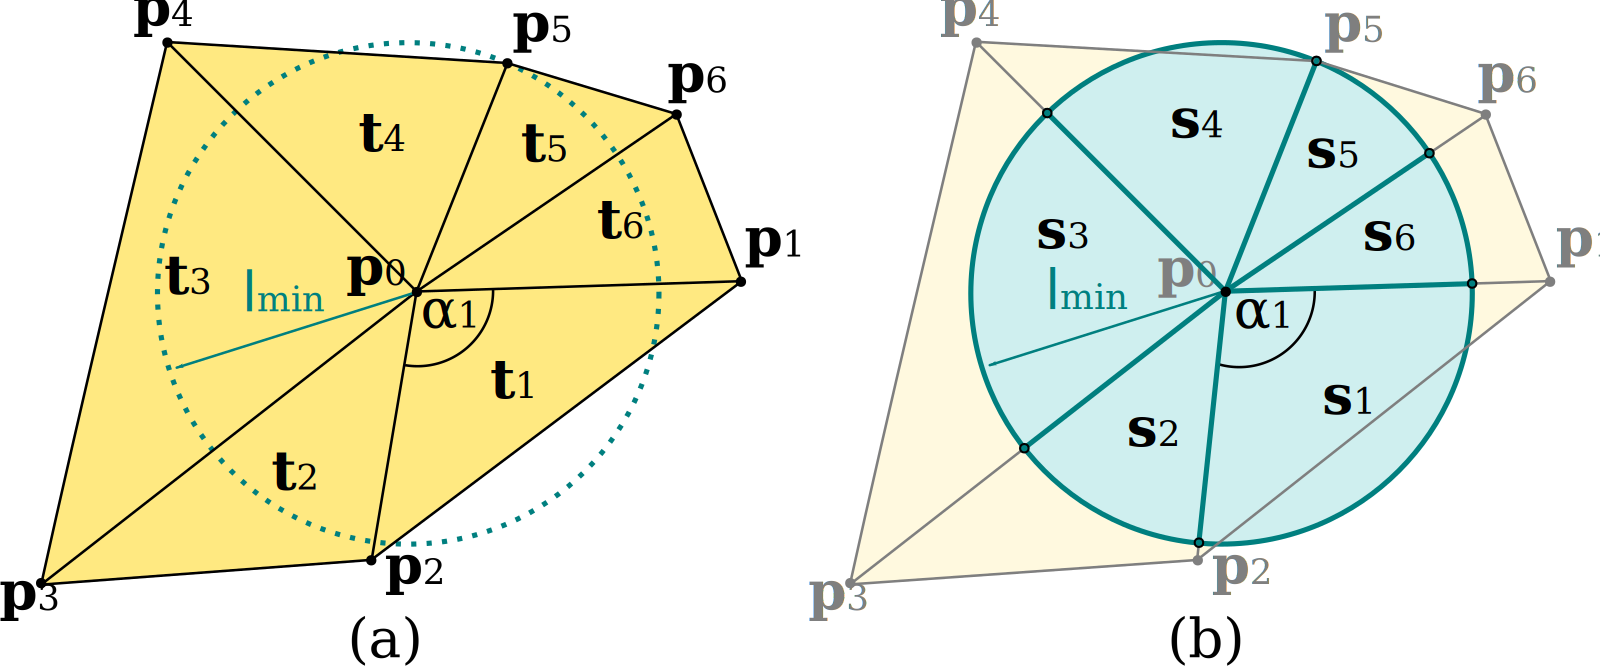
\includegraphics[width=1.0\linewidth]{figures/geodesicDisc.png}}
	{\caption[One-ring and geodesic disc]{A typical configuration of one-ring neighborhood $\bN_v$, described by (a) the six irregular triangular faces $\bt_i$ in sand color, which are defined by the six neighboring points $\bp_i$, which are all adjacent to the center point $\bp_0$; the smallest edge length $\elm = \elm(\bp_5) = |\bp_5 - \bp_0|$ illustrated with a teal arrow as the radius of the geodesic disc $\bO_v$, drawn as a dotted circle, also in teal color; and $\alpha_1$ as the central angle of $\bt_1$ (b) the complete geodesic disc $\bO$ composed of all six of the circular sectors $\bs_i$ which it circumscribes.}\label{fig:geodesicDisc}}
\end{figure}%

Furthermore, to ensure that the filter window size remains static for the duration of each convolution\todoResearch{call to question the importance of global minimum edge length in light of the typo found in source}, we define the global minimum edge length as
%
\begin{equation}
	\gelm := \min\left \{\elm(\bp_0) \;|\; \bp_0 \in \bM\,\right \}
	\label{eq:globalMinimumEdgeLength}
\end{equation}%
\nomenclature[jc]{$\gelm$}{the shortest edge length in $\bM$}%
%
and then use $\gelm$, the shortest edge length between any pair of adjacent points in the triangle mesh $\bM$, in lieu of the local minimum edge length $\elm(\bp_i)$, as the radius of the geodesic disc for all neighborhoods in all the following equations presented in this chapter.

%
%
%
\section{Interior Angles}
\label{ch4sIA}
Having determined the global minimum edge length $\gelm$ in the previous section, we may now consider the next steps in calculating \Fors{t}. Because we intend to use the area of each circle sector $\bs_i$ comprising the geodesic disc $\bO_v$ as weights upon the scalar field $\bF$ for averaging the function values first per sector, and then per neighborhood, we must initially calculate for use in those later computations, the central angles $\alpha_i$ of each triangular face $\bt_i$ in the neighborhood $\bN_v$. These central angles may be obtained by applying the Law of Cosines~\cite{Weisstein19e}, which would yield
%
\begin{equation}
	\alpha_i := cos^{-1}\left (\frac{|\bp_0 - \bp_{i}|^2 + |\bp_0 - \bp_{\sipo}|^2 - |\bp_i - \bp_{\sipo}|^2}{2\cdot|\bp_0 - \bp_{i}|\cdot|\bp_0 - \bp_{\sipo}|}\right )
\end{equation}
%
or more compactly:
%
\begin{equation}
	\alpha := cos^{-1}\left (\frac{\ell_c^2 + \ell_b^2 - \ell_a^2}{2\cdot\ell_c\cdot\ell_b}\right )
	\label{eq:alphaFromEdgeLengths}
\end{equation}%
\nomenclature[ka]{$\alpha$}{the central angle of circle sector $\bs_i$}%

Also, as it is our intention to interpolate and extrapolate the function values in relation to the distances between them and each of their adjacent points in the current neighborhood, we will be required to perform some calculations one side of the sector-bisecting line at a time, as will be discussed in detail later, in Section~\ref{ch4sWM}. But now, having computed the central angles $\alpha$, we can calculate the other interior angles $\beta$, in relation to $\gelm$ and opposite the bisecting line, using the line tangent to the circle sector at the bisecting line, to create two proxy right triangles, which together comprise the larger isosceles triangle which circumscribes the sector $\bs_i$. Next, we can to apply the third angle theorem\footnote{otherwise known as the Angle-Angle-Angle Theorem, abbreviated as AAA}~\cite{Weisstein19f} with $\alpha/2$, to calculate $\beta$ as defined in the formula
%
\begin{equation}
	\beta := \Big(\frac{\pi}{2} - \frac{\alpha}{2}\Big) = \frac{(\pi - \alpha)}{2}
	\label{eq:betaFromHalfAlpha}
\end{equation}%
\nomenclature[kb]{$\beta$}{the third angle with $\frac{\alpha}{2}$ and $\frac{\pi}{2}$}%
\nomenclature[kc]{$\bp'_j$}{also $\bp'_{\sjpo}$, the corners of the isosceles triangle circumscribing the circle sector, the intermediate location to where $f_j$ is first interpolated or extrapolated}%

Figure~\ref{fig:anglesAndCenterOfGravity} (a) extends Figure~\ref{fig:geodesicDisc} by focusing on the circle sector $\bs_1$, showing the triangular face $\bt_1$, angles $\alpha$ and $\alpha/2$, the bisecting line, the two angles $\beta$ with the tangent line, proxy right triangles defined by the points $\bp'_1$ and $\bp'_2$ used in their calculation, and additionally, the center of gravity which is discussed in detail in the next section.

%
%
%
%
\section{Area \& Center of Gravity}
\label{ch4sACG}
The next step towards the goal of computing the \wmfv{s} of the circle sectors $\bs_i$, is to calculate for each sector, the area $A$ and the distance $\check{\ell}$ from the center point $\bp_0$ along the bisecting line to the center of gravity $\bc$. Because a circle sector may be defined entirely by its radius and central angle~\cite{Weisstein19d}, having now calculated the radius as $\gelm$ in Section~\ref{ch4sSEL} and the central angle $\alpha$ in Section~\ref{ch4sIA}, the area of a sector can be calculated using the formula
%
\begin{equation}
	A := \frac{\left (\,\gelm\,\right )^2\alpha}{2}
	\label{eq:circularSectorArea}
\end{equation}

Similarly $\check{\ell}$, the distance from the center point $\bp_0$ along the bisecting line to the center of gravity $\bc$, can be calculated directly using the formula
%
\begin{equation}
	\check{\ell} := \frac{4\:\gelm\:\sin(\frac{\alpha}{2})}{3\,\alpha}
	\label{eq:distToCoG}
\end{equation}%

Figure~\ref{fig:anglesAndCenterOfGravity} (a) extends Figure~\ref{fig:geodesicDisc} by enhancing the circle sector $\bs_1$ to illustrate the center of gravity $\bc$ and $\check{\ell}$, the distance along the bisecting line from $\bp_0$ to $\bc$. In general, while holding the radius constant, the closer to $\pi/2$ the central angle $\alpha$ becomes, the longer the distance $\check{\ell}$ will be.

\begin{figure}[ht]
\ffigbox
	{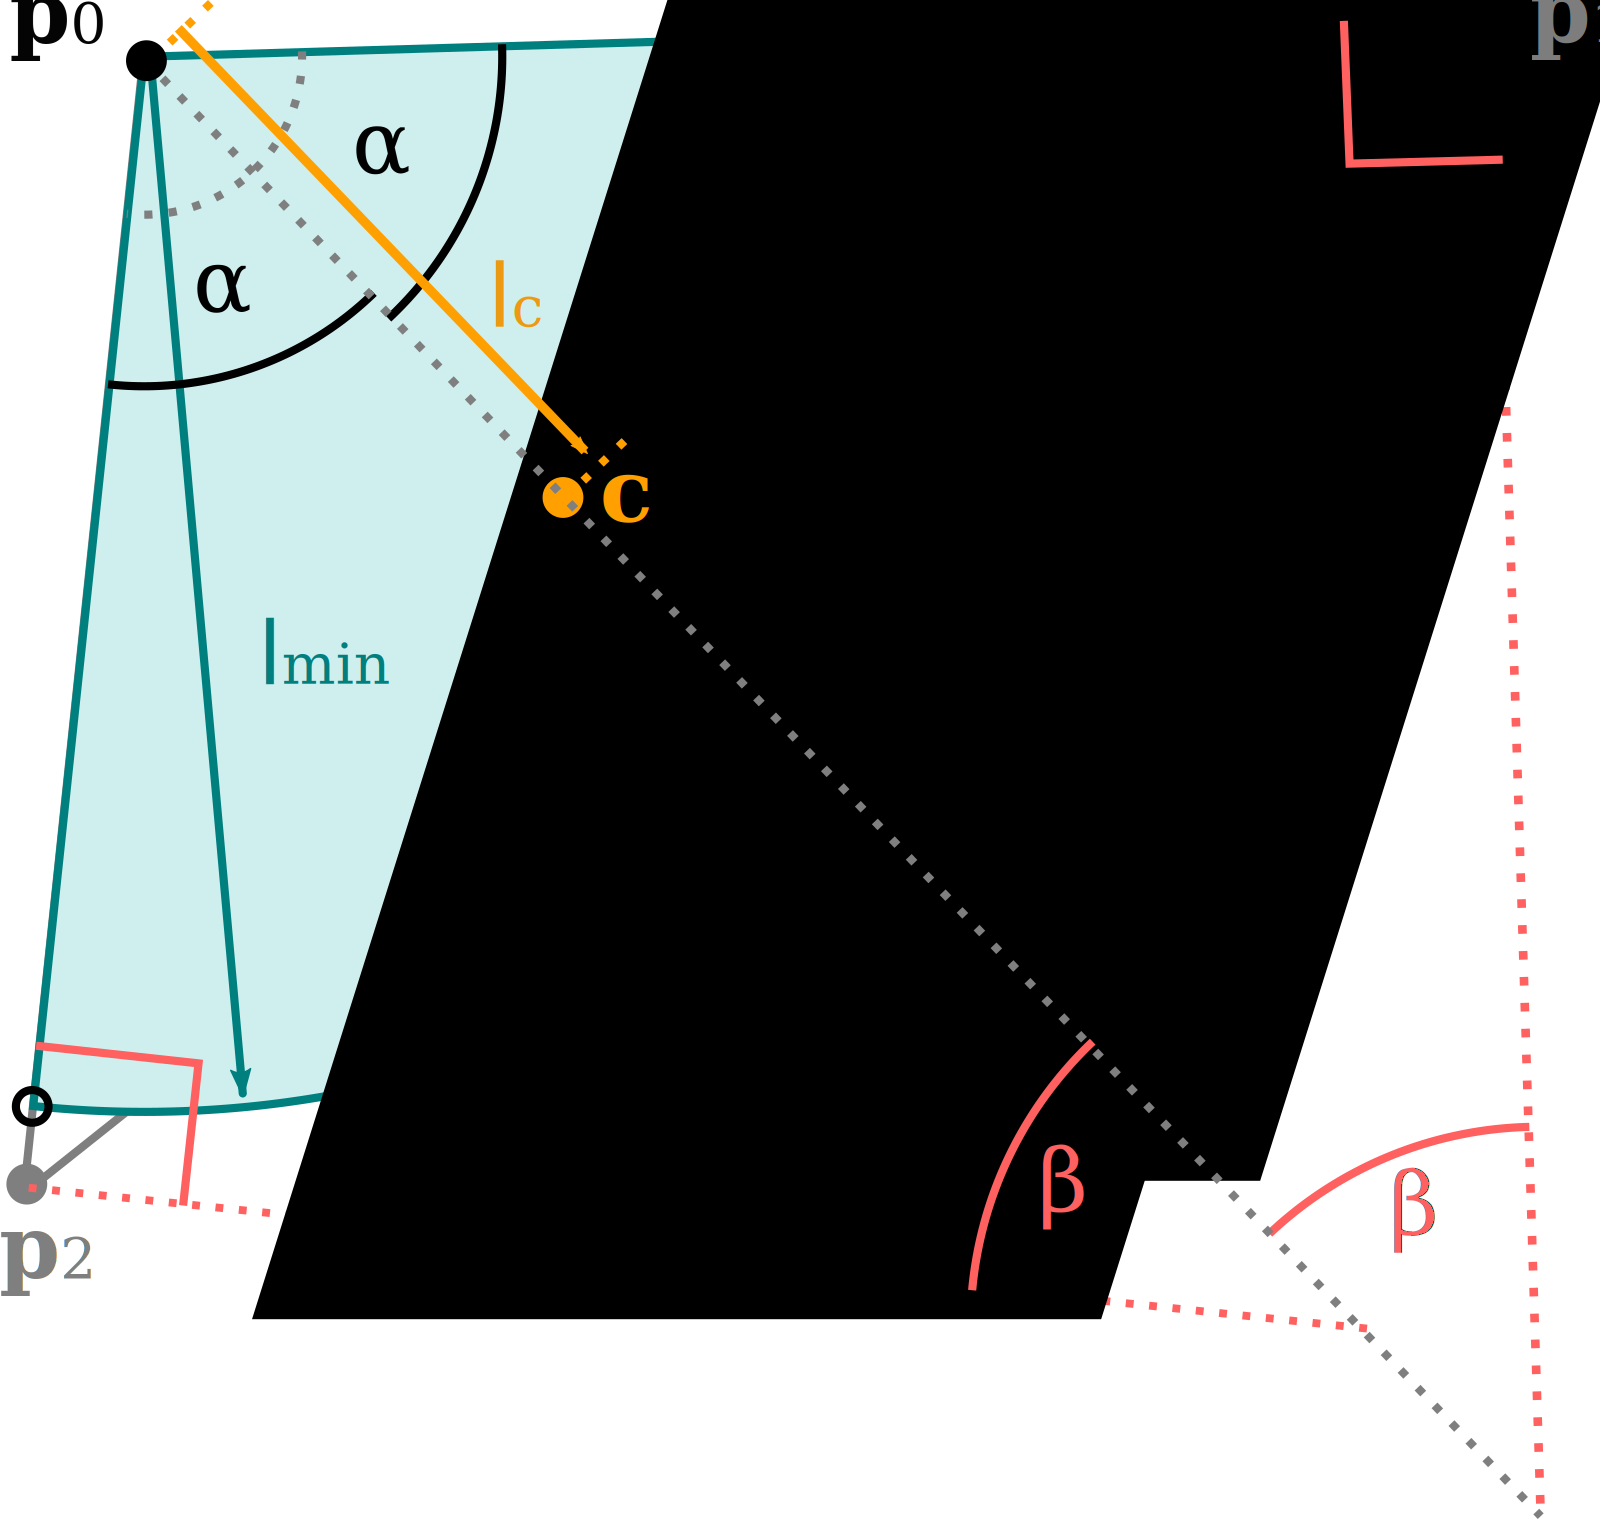
\includegraphics[width=0.8\linewidth]{figures/anglesAndCenterOfGravity.png}}
	{\caption[Angles and Center of Gravity]{An enhanced view of Figure~\ref{fig:geodesicDisc}, focusing on (a) the circle sector $\bs_1$, showing the triangular face $\bt_1$ and points $\bp_1$ and $\bp_2$ in gray, with $\alpha$ and the bisecting line in gray dots. In coral color is the center of gravity $\bc$ and $\check{\ell}$, the distance to it from $\bp_0$ along the bisecting line. Shown in sand color are the angles $\beta$, with the proxy right triangles defined by the points $\bp'_1$ and $\bp'_2$ used in their calculation (b) an example of a face and sector requiring both interpolation and extrapolation of its function values}\label{fig:anglesAndCenterOfGravity}}
\end{figure}%

%
%
%
%
\section{Interpolation \& Extrapolation}
\label{ch4sIE}
With the goal of computing the \wmfv{s} of the circle sectors $\bs_i$ by interpolating and extrapolating the function values from their points towards the center of gravity of each sector $\bc$, in Section~\ref{ch4sSEL} we calculated the global minimum edge length $\gelm$, then in Section~\ref{ch4sIA} we calculated the interior angle $\beta$; both of which are constant between the two halves of the circle sector. So now, given that information, we can obtain the sector-wise constant ratio $\zeta$, which will be used to scale the function values at the points $\bp_i$, to the interpolated or extrapolated values at the corners of the circumscribing isosceles triangle $\bp'_i$, by applying the Law of Sines~\cite{Weisstein19g} and ascribing
%
\begin{equation}
	\zeta := \frac{\gelm}{\sin\left (\beta\right )} = \frac{|\bp'_i - \bp_0|}{\sin\left (\pi/2\right )} = |\bp'_i - \bp_0|
	\label{eq:zeta}
\end{equation}%
\nomenclature[la]{$\zeta$}{sector-wise constant ratio for interpolation derived from Law of Sines}%

For the next few steps in the process of interpolating and extrapolating the function values, we must begin calculating for each half of the circular sector individually, because the points $\bp_j$ and $\bp_{\sjpo}$ are likely\footnote{One need only to look at Figures~\ref{fig:geodesicDisc} or~\ref{fig:anglesAndCenterOfGravity} for an example of why that may be.} at different distances from the center point $\bp_0$. Therefore, while the index $i$ will remain the index of the circle sector $\bs_i$, we will now use the index $j$ to denote the side of the bisecting line, defined by its point $\bp_j$ or $\bp_{\sjpo}$. 

Next, by dividing the sector-wise constant ratio $\zeta$ by the distances to the original points $\ell_j$ and $\ell_{\sjpo}$, we can determine the scalar values with which we can multiply the function values $f_j$ and $f_{\sjpo}$ in order to interpolate or extrapolate them to the corners of the circumscribing isosceles triangle at points $\bp'_j$ and $\bp'_{\sjpo}$. Therefore, these two scalar values are defined as
%
\begin{align}
	\tilde{\ell}_j & := \kern2pt\frac{\zeta}{\kern2pt\ell_j\kern2pt}\kern1pt = \kern3pt\frac{\zeta}{|\bp_j - \bp_0|}
	\label{eq:distanceIForInterpolation}\\
	\tilde{\ell}_{\sjpo} & := \frac{\zeta}{\ell_{\sjpo}} = \frac{\zeta}{|\bp_{\sjpo} - \bp_0|}
	\label{eq:distanceIp1ForInterpolation}
\end{align}%
\nomenclature[lb]{$\tilde{\ell}_j$}{also $\tilde{\ell}_{\sjpo}$, the distances for interpolation of $f_j$ and of $f_{\sjpo}$ towards $f_0$}%

Then, by taking the function values\footnote{\fors{T} is agnostic to the meaning of information represented by the data stored as function values in scalar fields, therefore, it can similarly convolve any such data. However, because the filter was designed to only convolve scalar fields, any multi-dimensional data, such as RGB color, must be processed individually as independent scalar fields.} from the scalar field $\bF$, and summing the products of the multiplications between the function values $f_j$, and $f_{\sjpo}$ and their scalar values $\tilde{\ell}_j$ and $\tilde{\ell}_{\sjpo}$, plus the product of the multiplication between the function value at the central point $f_0$ and the complement of each side's scalar value, we can now interpolate and extrapolate the function values at $\bp'_j$ and $\bp'_{\sjpo}$ as
%
\begin{align}
	f'_j & := f_0\,(1 - \tilde{\ell}_j) + f_j\,\tilde{\ell}_j
	\label{eq:interpolatedFi} \\
	f'_{\sjpo} & := f_0\,(1 - \tilde{\ell}_{\sjpo}) + f_{\sjpo}\tilde{\ell}_{\sjpo}
	\label{eq:interpolatedFip1}
\end{align}%
\nomenclature[lc]{$f'_j$}{also $f'_{\sjpo}$, the interpolated values of $f_j$ and $f_{\sjpo}$ toward $f_0$}%

Figure~\ref{fig:interpolatedFunctionValues} illustrates a 3D-projected, enhanced view of the circle sector $\bs_1$, continuing with the example introduced in Figure~\ref{fig:geodesicDisc}. Drawn above the points $\bp_0$, $\bp_1$, and $\bp_2$ are the three function values $f_0$, $f_1$, and $f_2$ from the scalar field $\bF$, with the heights indicative of each function value's magnitude. Also shown are the extrapolated function values $f'_0$, and $f'_1$ above the corners of the isosceles triangle $\bp'_1$, and $\bp'_1$, as well as the dotted lines illustrating the vectors on which the extrapolated values were calculated. Furthermore, it illustrates the process of interpolating the extrapolated function values towards each other, and then again towards the center of gravity, which is a topic covered in the next section.

\begin{figure}[ht]
\ffigbox
	{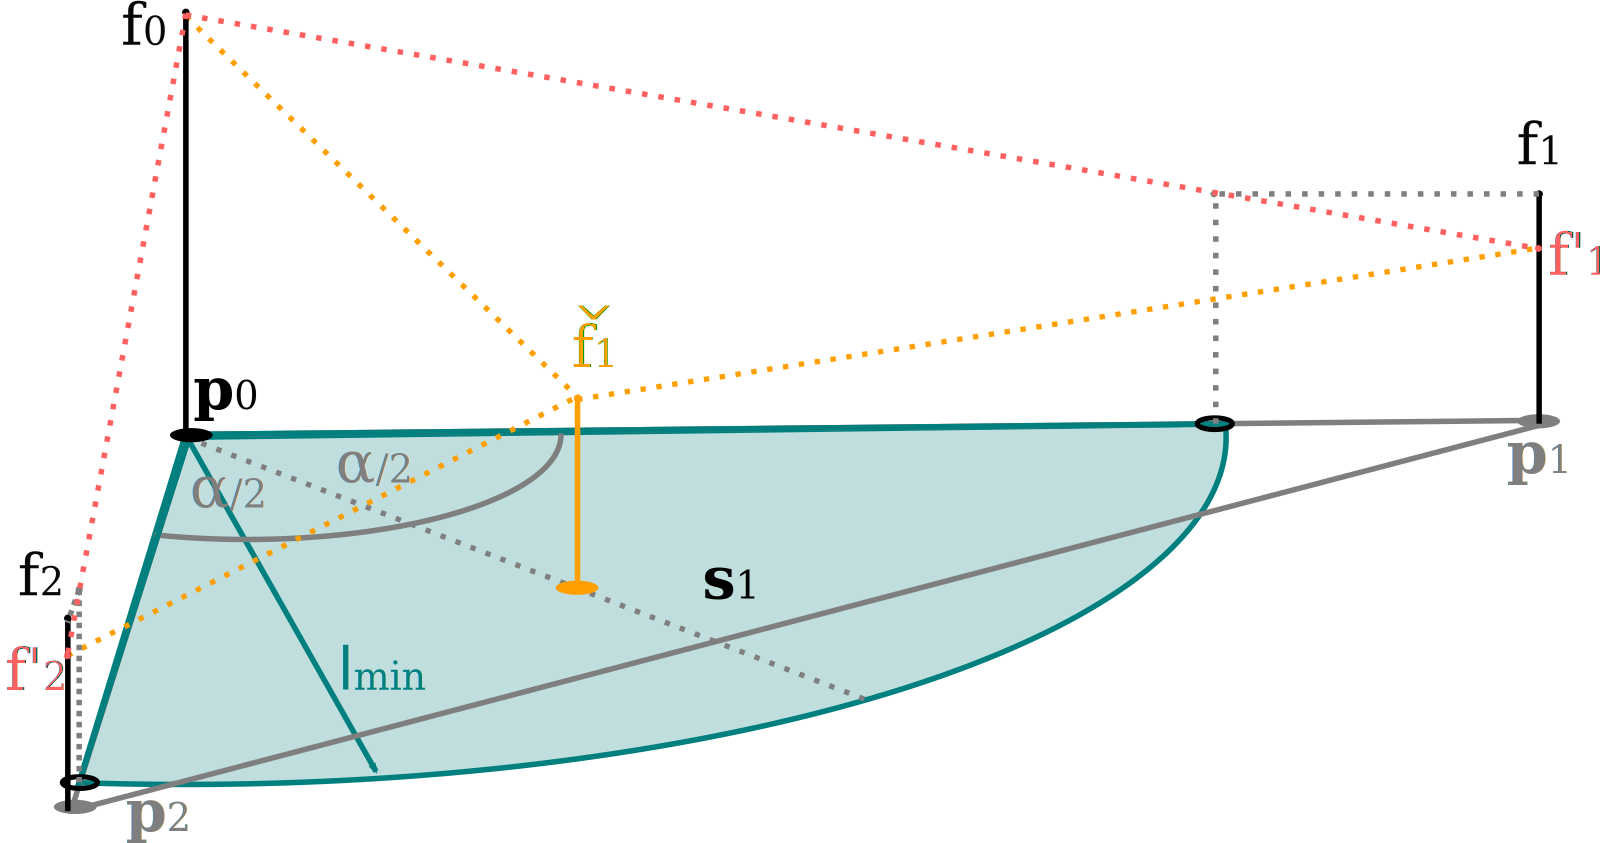
\includegraphics[width=1.0\linewidth]{figures/interpolatedFunctionValues}}
	{\caption[Interpolation of Function Values toward the Center of Gravity]{An enhanced view...}\label{fig:interpolatedFunctionValues}}
\end{figure}

%
%
%
%
\section{Weighted Means}
\label{ch4sWM}
Now that we have, in Section~\ref{ch4sACG}, calculated the distance to the center of gravity of each circle sector as $\check{\ell}$, and then in Section~\ref{ch4sIE}, computed the two function values interpolated or extrapolated to the corners of the isosceles triangle circumscribing the circle sector, $f'_j$ and $f'_{\sjpo}$, we are now poised to begin the computation of the \wmfv{s}, first for each circle sector $\bs_i$, then for the entire geodesic disc $\bO_v$, and finally iteratively convolving \Fors{t} over the entire mesh to generate the smoothed, scalar field of \wmfv{s} $\bF'$.

The next step then, is to calculate the \wmfv{} at the center of gravity $\bc$, of a circle sector $\bs_i$. That entails first interpolating the extrapolated function values towards each other, to the point where the tangent line intersects the arc of the circle sector, which is exactly the distance of $\gelm$ away from $\bp_0$. It is also always exactly half way between the two proxy points $\bp'_j$ and $\bp'_{\sjpo}$, so that interpolation always coincides with calculating the mean of the two function values. Therefore, by taking the equation for interpolation as was defined in Section~\ref{ch2sBTssGsssIE}, and used in Algorithms~\ref{interpolatedFi}, and~\ref{interpolatedFip1}, then applying $\gelm$ as the domain, and the difference between the original function value at the central point $\bp_0$ and the mean of the interpolated and extrapolated function values as the range, we obtain the formula
%
\begin{equation}
	\check{f} := f_0\,(1 - \check{\ell}) + \frac{(f'_j + f'_{\sjpo})\,\check{\ell}}{2}
	\label{eq:weightedMeanAtCoGatSector}
\end{equation}%
\nomenclature[ma]{$\check{f}$}{the weighted mean function value at $\bc$ of $\bs_i$}
%
which is used to calculate the \wmfv{} at the center of gravity $\check{f}$, and therefore represents the \wmfv{} over the entire circle sector.

Figure~\ref{fig:interpolatedFunctionValues} illustrates a 3D-projected, enhanced view of the circle sector $\bs_1$, continuing with the example introduced in Figure~\ref{fig:geodesicDisc}. The \wmfv{} $\check{f}_1$, which represents the entire circle sector, is drawn at its interpolated value above the center of gravity $\bc$. The figure also shows the dotted lines illustrating the interpolation from the extrapolated function values $f'_1$ and $f'_2$, as well as the details pertaining to their own computations, as discussed in detail in Section~\ref{ch4sIE}.

Finally, we can multiply each \wmfv{} located at each circle sector's center of gravity $\check{f}_i$, by each sector's area $A_i$, to obtain the volume of function value over the entire circle sector. Then by dividing the sum of all those volumes by the total area of the geodesic disc $\bO_v$, we can compute
%
\begin{equation}
	f'_v := \frac{\sum A_i\check{f}_i}{\sum A_i} \quad \forall i \in \{1,\ldots,\,|\bN_v|\}
	\label{eq:meanFuncValAtPv}
\end{equation}%
\nomenclature[mb]{$f'_v$}{the one-ring weighted mean function value at $\bp_v$}
%
the one-ring weighted mean\footnote{\fors{T} can be modified to use the median operation, instead of the mean, by using all the equations except Equation~\ref{eq:meanFuncValAtP0} and then sorting the results of Equation~\ref{eq:weightedMeanAtCoGatSector}. The details of which can be found by the original publication ~\cite[s.~3.2]{Mara17}, but as it was not implemented in GPGPU for this thesis, we exclude the details here.} function value for $\bp_v$, which is the center point $\bp_0$ of the neighborhood $\bN_v$.

Figure~\ref{fig:funcValVolumes} illustrates a 3D-projected view of the geodesic disc $\bO$, as introduced in Figure~\ref{fig:geodesicDisc}, with volumes of interpolated function value over each circle sector, which shall be summed together, then divided by the total area of the geodesic disc in order to obtain the the one-ring \wmfv{} $f'_v$ at point $\bp_v$.

\begin{figure}[ht]
\ffigbox
	{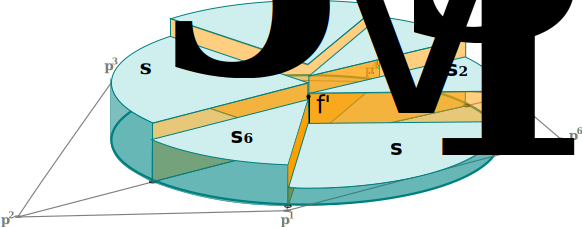
\includegraphics[width=1.0\linewidth]{figures/funcValVolumes.png}}
	{\caption[Weighted Mean Function Value $f'_v$at $\bp_v$]{The geodesic disc $\bO$, as introduced in Figure~\ref{fig:geodesicDisc}, with volumes of interpolated function values over each circle sector $\bs_i$, which shall be divided by each sector's area $A$ in order to obtain the the one-ring weighted mean function value $f'_v$ at $\bp_v$.}\label{fig:funcValVolumes}}
\end{figure}

All that remains for \Fors{t}, is to convolve the filter over the entire set of points comprising the mesh $\bP$, then to collect the computed one-ring \wmfv{s} in the set
%
\begin{equation}
	\bF' :=  \left \{\:f'_v \mid v \in \mathbb{N}, \;\text{and}\; 1\leq v \leq |\bP|\:\right \}
	\label{eq:zeta}
\end{equation}%
\nomenclature[mc]{$\bF'$}{a scalar field, a set of \wmfv{s}, the product of convolving \fors{t}}%
%
which can be either be used in lieu of $\bF$ in subsequent convolutions, or simply taken as the final product of all the processes described in this chapter. As with any smoothing filter, one can convolve \fors{t} for any number of iterations, thus producing a smoothing effect with increasing intensity in relation to the number of convolutions. But while there is no upper limit to the number of convolutions one may apply, the function values will all eventually converge at the global mean average function value. More details can be found in Section~\ref{ch3s2}.\todoCitation{mara on iteration count vs filter size}.\todoReword{choosing convolution counts}

%
%
%
%
\section{Summary}
\label{ch4sS}
In this chapter we presented the mathematical grounding for the as-yet-unpublished, updated version of \Fors{t}, which since its original publication~\cite[s.~3.2]{Mara17}, now utilizes the entire area of each sector $\bs$ of the geodesic disc $\bO$ centered at each point $\bp_v$ in the mesh $\bM$, in order to calculate the weighted average of all the function values in its one-ring neighborhood. First, we illustrated in detail how one can calculate the global minimum edge length $\gelm$, and for each circle sector in the one-ring neighborhood $\bN$, the interior angles $\alpha$ and $\beta$, the area $A$, and the distance $\check{\ell}$ from the center point to the center of gravity $\bc$. Next, we provided the equations for interpolating and extrapolating the three function values $f_0$, $f_j$, and $f_{\sjpo}$ to the center of gravity, using the sector-wise constant ratio $\zeta$ in order to obtain the \wmfv{} $\tilde{f}$ for each sector. Finally, we computed the \wmfv{} $f'_v$ at the central point $\bp_v$, which is collected into the set $\bF'$. Convolving this filter at each point in the mesh, with the scalar field of function values $\bF$, for any number of iterations, thus produces a smoothing effect with increasing intensity in relation to the number of iterations.

In the next chapter, we will develop the serial algorithms required for implementing \Fors{t}, to be utilized as the foundation for the parallel algorithms to described in detail in Chapter~\ref{6}.

\chapter{Fast One-Ring Smoothing: Serial Algorithms}
\label{ch5}
In the previous chapter we presented the mathematical grounding for an improved version of \Fors{t} as it is currently implemented within the GigaMesh framework. Now in this chapter, we will use mathematical pseudo-code to combine all of the equations from Chapter~\ref{ch4}, Equations~\ref{eq:localMinimumEdgeLength} through~\ref{eq:meanFuncValAtPv}, into a serial algorithm, with the goal of preparing the basis from which we will subsequently design the parallel algorithm presented in Chapter~\ref{ch6}.

%
%
%
%
\section{An Algorithm in Three Parts}
\label{ch5sATP}
The serial algorithm defined in this chapter requires that the membership of all one-ring neighborhoods first be discovered before one is ever able to begin convolving the filter, because the total efficiency of the algorithm relies on iterating over the family of sets of neighborhoods $\bN$, as will be made clear in Sections~\ref{ch5sCEL}, and~\ref{ch5sCF}, while the underlying data structure of \tdd{} typically only stores a mesh $\bM$ as the superset of the two separate sets, $\bP$ of points, and $\bT$ of triangular faces, completely ignorant of the adjacency between faces or even the concept of neighborhoods. 

Also critical to the total efficiency of the filter, is the pre-calculation of the edge lengths between all pairs of adjacent points, whose magnitudes never change, regardless of the number of convolutions being applied. This importance stems from how all edge lengths are used in computation during the loop for convolving the filter, which we will refer to as the principle filter going forward, at least five times per convolution, and tens times per convolution for the majority of points, which are non-border pairs, whose relationships are duplicated in adjacent neighborhoods.\todoReference{appendix on mesh face to point ratio goto2}%
\nomenclature[]{``the principle loop''}{the loop for convolving the filter}%

Therefore, in order to maximize the efficiency of \Fors{t}, it is crucial to split the algorithm into three distinct parts: first building neighborhoods, then calculating edge lengths, and finally convolving the filter, while storing the results of the first two parts, so that they may be used during the iterative convolutions of the third part; the result being a massive increase in efficiency by greatly reducing the number of operations-per-convolution required by the filter.
\todoBackground{add convolution and convolve to background}
\todoBackground{memory vs speed cost compromise}

%
%
%
%
\section{Building Neighborhoods}
\label{ch5sBN}
Before convolving \fors{t}, one must initially discover all the points in the mesh $\bp_i$ which comprise each neighborhood $\bN_v$, then store those connections in the family of sets $\bN$. That is the purpose of Algorithm~\ref{alg:serialBuildNeighborhoods}. Despite the fact that building $\bN$ outside of the principle loop adds an additional $6\cdot|\bT|$ operations to the total, instead, Algorithm~\ref{alg:serialCalculateEdgeLengths} becomes able to exploit the explicit connections stored in $\bN$, in order to vastly reduce its complexity from $|\bP|^{|\bT|}$, down to only $|\bP|^{\bar{n}}$, where $\bar{n}$ is the average size of all neighborhoods, which with acquired \tdd{}, will typically evaluate to approximately 6.\todoReference{Appendix on border vs nonborder ,and beighborhood size} Also, as we will see in Section~\ref{ch5sCF}, when $\tau$ is the user-defined number of convolutions to perform, the complexity of the principle loop can be meaningfully reduced to only $\tau^{|\bP|^{2\cdot\bar{n}}}$, down from the $\tau^{|\bP|^{(2\cdot|\bT|)}}$ that would have been necessary, had the neighborhoods not already been discovered and the procedure been otherwise required to discover the members of $\bN_v$ in each convolution.%
\nomenclature[na]{$\tau$}{the user-defined number of convolutions to perform}%
\todoBackground{complexity, big O notation}

Figure~\ref{fig:unionsOfSimpleBuildNeighborhoods} describes a very simple mesh consisting of just two faces and four points, similar to what is illustrated in Figure~\ref{fig:triangularFaces}. The arrows represent the union operation between a point and a neighborhood, and are colored to match the face from where the point had come. It should be noted that the two pairs of arrows pointing from $\bp_2$ to $\bN_3$, and $\bp_3$ to $\bN_2$, indicate that both of these union operations occur twice, originating one each from both faces, but because of the uniqueness property of sets, the duplicated operations are wholly inconsequential to the the final membership of either neighborhood.

\begin{figure}[ht]
	\includestandalone[width=\textwidth]{figures/tikz/unionsOfSimpleBuildNeighborhoods}
	{\caption[unionsOfSimpleBuildNeighborhoods]{A very simple mesh consisting of just two faces and four points, similar to what is illustrated in Figure~\ref{fig:triangularFaces}. The face $\bt_1$ is in sand color, and $\bt_2$ is in coral color. The arrows represent the union operation between a point into a neighborhood, and are colored to match the face from where the point had come. The two pairs of arrows pointing from $\bp_2$ to $\bN_3$ and $\bp_3$ to $\bN_2$ are colored in teal to highlight the fact that these union operations occur twice.
}\label{fig:unionsOfSimpleBuildNeighborhoods}}
\end{figure}

Also notice in Figure~\ref{fig:serialBuildNeighborhoods}, that the union operation is performed exactly twice per point per face; that is, once each between the neighborhood of the center point and a neighboring point, for a total of six times per face. For example: the triangular face $\bt_2$ contains the point $\bp_4$, therefore the union operation is performed on $\bN_4$ at least two times, once for each of the other members of point $\bt_2$: $\bp_2$, and $\bp_3$. This realization will influence the design of the parallel variant of the algorithm, as described in Section~\ref{ch6sBNPssABN}.


In Algorithm~\ref{alg:serialBuildNeighborhoods}, the function \textit{serialBuildNeighborhoods} describes iterating over every triangular face $\bt$ in $\bT$, then for each face's three corner points, perform the union operation between the neighborhood centered at the point, and the other two points which are adjacent to the central point. After processing every face, the result becomes a fully populated family of sets $\bN$, storing the connections between every neighbor of every neighborhood in the mesh $\bM$.

\begin{algorithm}[ht]
	\algotitle{Serial Algorithm for Building Neighborhoods}{saBN.title}
	\DontPrintSemicolon
	\SetCommentSty{small}
	\SetKwFor{For}{for}{:}{}
	\SetKwProg{Func}{Function}{}{}
	\SetKwInOut{Input}{Input}\SetKwInOut{Output}{Output}

	\Input{the set of all triangular faces $\bT$}
	\Output{the family of sets of discovered neighborhoods $\bN$}

	\bigskip
\nl	\Func{serialBuildNeighborhoods($\bT$)}{\label{sbn1}
\nl		\For(\tcc*[f]{$\bt = \left \{\bp_a, \bp_b, \bp_c\right \}$}){$\bt \in \bT$}{\label{sbn2}
\nl			\ProgSty{union($\bN$, $\bp_a$, $\bp_b$, $\bp_c$)}\;\label{sbn3}
\nl			\ProgSty{union($\bN$, $\bp_b$, $\bp_a$, $\bp_c$)}\;\label{sbn4}
\nl			\ProgSty{union($\bN$, $\bp_c$, $\bp_a$, $\bp_b$)}\;\label{sbn5}
		}
	}

	\bigskip
\nl	\Func{union($\bN$, $a$, $b$, $c$)}{\label{sbn7}
\nl		$\bN_a \leftarrow \bN_a \cup \{b,\,c\}$\;\label{sbn8}
	}
	\caption{Serial algorithm for building the family of sets $\bN$, from all discovered members of each neighborhood in the mesh\label{alg:serialBuildNeighborhoods}}
\end{algorithm}%

The function \textit{union} is defined separately in Algorithm~\ref{alg:serialBuildNeighborhoods} for two reasons: the first reason is that when separated, it becomes very clear that the union operation behaves similarly for all three permutations\footnote{In general, a set of three numbers has six permutations, however, here only the first index is important, and the order of the second two parameters are arbitrary due to the commutative property of the union operation, resulting in only 3 distinct possibilities} of corners, and indeed it is only the order of the indices which changes; the second reason is that this signature will match more closely that of its parallel variant, to be defined in Algorithm~\ref{alg:parallelBuildNeighborhoods}, which will require the union operation to remain separate.
\todoBackground{Commutative property of union operation}

%
%
%
%
\section{Calculating Edge Lengths}
\label{ch5sCEL}
Having now built in the previous section the family of sets of neighborhoods $\bN$, we can advance to the next step, Algorithm~\ref{alg:parallelCalculateEdgeLengths}, which iterates over each pair of neighbors comprising $\bN$, with the goal of building a set of pre-calculated edge lengths $\bE$, as well as determining the global minimum edge length $\gelm$; both being essential parameters of Algorithm~\ref{alg:serialConvolveFilter}.

As shown in Equation~\ref{eq:defineEdgeLengthPoint}, the calculation of an edge's length requires taking the L2-norm of the difference between two points, which itself involves using the square root operation. In modern software, the square root operation is performed by computing ``Newton's Iteration'', or ``Newton's method''\todoCitation{software uses Newton's iteration for sqrt}, which is essentially multiple iterations of the so-called, ``recurrence equation''.~\cite{Weisstein19b}\todoCitation{Newton's iteration uses recurrence equation} The impact for \fors{t} is that the computation of a square root typically\todoReword{add footnote with desc and citation}\todoCitation{how slow is Newton's iteration compared to others} takes many more compute cycles than  any other binary or unary operation, thus taking more time to complete overall. In fact, because of the slowness of the square root operation, computing the L2-norm in order to calculate an edge's length is empirically the most costly operation performed by the filter\todoResearch{qualify, do experiment to prove how slow sqrt is, maybe make appendix entry about what it is and why it is so slow}. Therefore, it is imperative that we pay special attention to avoid unnecessary instructions to calculate an edge's length. For that reason, we define the symbol $\ellstar$ to represent the calculation of an edge's length using ``Newton's Iteration'', so that we may draw focus to its importance while remaining concise.%
\nomenclature[oa]{$\ellstar$}{the procedure of calculating an edge's length using ``Newton's Iteration'', the most costly operation in the Fast One-Ring filter, due to use of $\sqrt{(\cdot)}$}

In Algorithm~\ref{alg:serialCalculateEdgeLengths}, the function \textit{serialCalculateEdgeLengths} iterates over a set of nested loops which considers each neighbor $\bp_i$ of each neighborhood $\bN_v$, in order to calculate the edge lengths between the center point $\bp_v$ and its neighboring points $\bp_i$. The result is then stored in the set $\bE$ using the pair of indices $v, i$ to reflect the structure of the family of sets of neighborhoods $\bN$. Finally, in each iteration, the value of the global minimum edge length $\gelm$ is updated to become the minimum between $\bE_{\sv{i}}$ and the current $\gelm$, ensuring that at the conclusion of the procedure, that no other edge length in $\bE$ will be shorter than $\gelm$.

\begin{algorithm}[ht]
	\algotitle{Serial Algorithm for Calculating Edge Lengths}{saCEL.title}
	\DontPrintSemicolon
	\SetCommentSty{small}
	\SetKwFor{For}{for}{:}{}
	\SetKwProg{Func}{Function}{}{}
	\SetKwInOut{Input}{Input}\SetKwInOut{Output}{Output}

	\Input{the set of all points $\bP$, \\
		the family of sets of discovered neighborhoods $\bN$}
	\Output{the set of pre-calculated edge lengths $\bE$, \\
		the global minimum edge length $\gelm$}

	\bigskip
	\Func{serialCalculateEdgeLengths($\bP$, $\bN$)}{
\nl		\For{$\bp_v \in \bP$}{\label{scel1}
\nl			\For{$\bp_i \in \bN_v$}{\label{scel2}
				\linespread{1.5}\selectfont
\nl				$\bE_{\sv{i}} \leftarrow |\bp_i - \bp_v|$\tcc*[r]{This is $\ellstar$ as in Eq:~\ref{eq:localMinimumEdgeLength}}\label{scel3}
\nl				$\gelm \leftarrow \min\left \{\gelm,\,\bE_{\sv{i}}\right \}$\tcc*[r]{Eq:~\ref{eq:globalMinimumEdgeLength}}\label{scel5}
			}
		}
	}
	\caption{Serial algorithm for calculating all the edge lengths between each pair of adjacent points in the mesh\label{alg:serialCalculateEdgeLengths}}
\end{algorithm}

Given the substantial impact of computing ${\ellstar}$, and the enormous number\footnote{``enormous'' $\approx2\cdot\left (|\bP|^{5\,\bar{n}}\right )$ as the non-border to border edge lengths converges to 2 with increasing mesh density, described in detail in the appendix}\todoResearch{update the 2 once the real value is known} of times an edge length is required in the computation of the \wmfv{s} per convolution of the filter, pre-calculating the set all of edge lengths $\bE$ outside of the principle loop becomes critical to the overall efficiency of the algorithm, despite the fact that it requires ${\ellstar}$ to be calculated and stored $|\bP|^{\bar{n}}$ times. It is of paramount importance for two reasons: the first reason is that without pre-calcuating every edge length, it would be otherwise impossible to calculate the global minimum edge length $\gelm$, which is used $|\bP|^{4\,\bar{n}}$ times in every convolution of the filter; the second reason is that by recording the results of every $\ellstar$ calculation in the set $\bE$, we are then able to completely exclude any further calculations of $\ellstar$ from the principle loop, and as can be seen in Algorithm~\ref{alg:serialConvolveFilter}, that reduces the total count of $\ellstar$ calculations performed by the filter from the $\tau^{|\bP|^{3\,\bar{n}}}$ had the procedure been required to calculate an edge length each time it was used during computation, down to only the initial $1\cdot |\bP|^{\bar{n}}$ pre-calculations; having now become completely independent of $\tau$ and significantly more efficient overall.%
\nomenclature[ob]{$\bE$}{a set of pre-calculated edge lengths}%
\todoBackground{memory vs speed cost compromise}
\todoBackground{border vs non-border edge lengths}

%
%
%
%
\section{Convolving the Filter}
\label{ch5sCF}
After having discussed in Section~\ref{ch5sBN}, the discovery and subsequent construction of the set of every one-ring neighborhood $\bN$, then in Section~\ref{ch5sCEL}, the set of pre-calculations of every edge length $\bE$, in this section, we present the third and final part of the serial algorithm for convolving \Fors{t}, which describes the remaining steps required to convolve the filter over a mesh. 

In Algorithm~\ref{alg:serialConvolveFilter}, the function \textit{convolveFilter} outlines how the convolutions of \fors{t} are performed for a user-defined number of times $\tau$, by convolving over each and every point $\bp_v$ in the set $\bP$. Then at each point, each neighboring point $\bp_i$ in the one-ring neighborhood $\bN_v$ is examined, in order to calculate the \wmfv{} $\check{f}$, as described in detail in Sections~\ref{ch4sIA} -~\ref{ch4sWM}, at the center of gravity of the circle sector defined by $\bp_v$ and $\bp_i$. Next, the \wmfv{} $f'_v$ is evaluated as the average of all the \wmfv{s} from each circle sector comprising the geodesic disc $\bO_v$, and is stored  in set $\bF'$, before the filter finally progresses to the next point in the mesh and its corresponding one-ring neighborhood.  Afterwards, one may efficiently convolve the filter, for as many number of convolutions as required to achieve the desired smoothing effect.

\begin{algorithm}[ht]
	\algotitle{Serial Algorithm for Convolving the Filter}{saCF.title}
	\DontPrintSemicolon
	\SetCommentSty{small}
	\SetKwFor{For}{for}{:}{}
	\SetKwProg{Func}{Function}{}{}
	\SetKwInOut{Input}{Input}\SetKwInOut{Output}{Output}

	\Input{the set of all points $\bP$, \\
		the family of sets of discovered neighborhoods $\bN$, \\
		the set of pre-calculated edge lengths $\bE$, \\
		the global minimum edge length $\gelm$, \\
		the set of function values $\bF$, \\
		the user-defined number of convolutions $\tau$}
	\Output{the set of one-ring \wmfv{s} $\bF'$}

	\bigskip
	\linespread{1}\selectfont
	\Func{serialConvolveFilter($\bP$, $\bN$, $\bE$, $\gelm$, $\bF$, $\tau$)}{
\nl		\For{$t\leftarrow 1\;\KwTo\;\tau$}{
\nl			\For{$\bp_v \in \bP$}{
\nl				\For{$\bp_i \in \bN_v$}{
					\linespread{1.5}\selectfont
\nl					$\kern-0.5pt\alpha \leftarrow cos^{-1}$
					\begin{Large}
						$\kern-6pt\left (\frac{\bE_c^2\,+\,\bE_b^2\,-\,\bE_a^2}{2\,\cdot\,\bE_c\,\cdot\,\bE_b}\right )$\tcc*[r]{Eq:~\ref{eq:alphaFromEdgeLengths}}
					\end{Large}\label{algSCFalpha}
					\linespread{1.2}\selectfont
\nl					$\kern0.00pt\beta \leftarrow (\pi - \alpha)\mathbin{/}2$\tcc*[r]{Eq:~\ref{eq:betaFromHalfAlpha}}\label{algSCFbeta}
\nl					$\kern-1.5ptA \leftarrow \Big(\gelm\,\Big)^2\kern-4pt\cdot\alpha\mathbin{/}2$\tcc*[r]{Eq:~\ref{eq:circularSectorArea}}\label{algSCFarea}
\nl					$\kern1.00pt\check{\ell} \leftarrow \big(4\cdot\gelm\cdot\sin(\alpha\mathbin{/}2)\big)\mathbin{/}3\,\alpha$\tcc*[r]{Eq:~\ref{eq:distToCoG}}\label{algSCFcog}
\nl					$\kern1.00pt\zeta \leftarrow \gelm\mathbin{/}\sin(\beta)$\tcc*[r]{Eq:~\ref{eq:zeta}}\label{algSCFzeta}
\nl					\For{$j \in {1,2}$}{\label{algSCFjloop}
\nl						$\tilde{\ell}_j \leftarrow \zeta\mathbin{/}\bE_j$\tcc*[r]{Eq:~\ref{eq:distanceIForInterpolation},~\ref{eq:distanceIp1ForInterpolation}}
\nl						$f'_j \leftarrow f_0\cdot(1 - \tilde{\ell}_j) + f_j\cdot\tilde{\ell}_j$\tcc*[r]{Eq:~\ref{eq:interpolatedFi},~\ref{eq:interpolatedFip1}}
					}
\nl					$\check{f} \leftarrow f_0\cdot(1 - \check{\ell}) + \big((f'_1 + f'_2)\cdot\check{\ell}\big)\mathbin{/}2$\tcc*[r]{Eq:~\ref{eq:weightedMeanAtCoGatSector}}\label{algSCFcheckf}
\nl					$\kern-2.0pt\tilde{f}_v \leftarrow \tilde{f}_v + A\cdot\check{f}$\tcc*[r]{Eq:~\ref{eq:meanFuncValAtPv}}\label{algSCFarea}
\nl					$\kern-4.0pt\tilde{A}_v \leftarrow \tilde{A}_v + A$\tcc*[r]{Eq:~\ref{eq:meanFuncValAtPv}}\label{algSCFtildearea}
				}
\nl				$f'_v \leftarrow \tilde{f}_v\mathbin{/}\tilde{A}_v$\tcc*[r]{Eq:~\ref{eq:meanFuncValAtPv}}\label{algSCFfprimev}
			}
\nl		$\bF' \leftarrow \left \{f'_1,\ldots,\,f'_{|\bP|}\right \}$\;\label{algSCF2ndlastLine}
\nl 	$\bF \leftarrow \bF'$\tcc*{smooth newest values every convolution}\label{algSCFlastLine}
		}
	}
	\caption{Serial algorithm for convolving \Fors{t}\label{alg:serialConvolveFilter}}
\end{algorithm}%
\nomenclature[pa]{$\tilde{f}$}{the total volume of function values over $\bO_v$}%
\nomenclature[pb]{$\tilde{A}$}{the area of $\bO_v$}%
\nomenclature[]{$\bF'$}{the set of one-ring \wmfv{s}}%

While the performance of Algorithm~\ref{alg:serialConvolveFilter} is much improved by the neighborhood building and pre-calculations performed in Algorithms~\ref{alg:serialBuildNeighborhoods} and~\ref{alg:serialCalculateEdgeLengths}, its strictly serial design prevents it from scaling in performance appropriately for the sizes of real-world, acquired \tdd{}, performing especially sluggishly for high numbers of convolutions on meshes with large amounts of triangulated points\todoReference{a specific experiment}; the very targets for which \Fors{t} is primarily intended.

%
%
%
%
\section{Summary}
\label{ch5sDN}
In this chapter, we presented the serial algorithms for implementing the improved version of \Fors{t}, as implemented within the GigaMesh framework. In Section~\ref{ch5sATP}, we discussed the motivation behind separating the algorithm into three parts, citing the substantial improvements to the over all efficiency of the filter. In Section~\ref{ch5sBN}, the considerations behind building a family of sets of neighborhoods are weighed, before presenting the function \textit{serialBuildNeighborhoods} in Algorithm~\ref{alg:serialBuildNeighborhoods}. Then in Section~\ref{ch5sCEL}, the significance of $\ellstar$ and the L2-norm calcuation is explained in context with modern implementations of the square root operation, before presenting function \textit{serialCalculateEdgeLengths} in Algorithm~\ref{alg:serialCalculateEdgeLengths}.   Then finally, in Section~\ref{ch5sCF}, Algorithm~\ref{alg:serialConvolveFilter} is presented with the function \textit{serialConvolveFilter} which implements the principle loop for convolving the filter over a mesh, for as many number of convolutions as required to achieve the desired smoothing effect.

Unfortunately, \Fors{t} is still yet entirely serial in design, therefore, we will in the next section, endeavor to explore this as-yet-unpublished algorithm in order to discover any manifestations of independent procedures worthy of exploiting with parallel processing, with the goal of improving the overall performance and scalability of the filter when it is implemented on a system capable of parallel computation.


\chapter{Fast One-Ring Smoothing: Parallel Algorithms}
\label{ch6}
 the previous chapter we presented the mathematical grounding for an improved version of \Fors{t} as it is currently implemented within the GigaMesh framework, and while it has improved accuracy in regards to the weights, it is still yet entirely serial in design, so that unfortunately, its performance suffers greatly under the complexity of modern mesh sizes, which with the current high resolution scanners in use, can grow to be MESH\_SIZES\todoResearch{mesh sizes}. In this chapter, we will now explore the serial version of this as-yet-unpublished algorithm, in order to design the parallel algorithm presented in Chapter~\ref{ch6}.

negotiate any instances of control or data dependency, and hopefully discover opportunities worthy of exploiting concurrency in order to improve its performance when implemented on a system capable of parallel computation.

\todoBackground{Data dependencies}
Following the pattern set in Section~\ref{ch5sSI}, the parallel algorithm for \Fors{t} also has three main parts. In contrast however, the parallel variant of each of the three serial parts are split further into subroutines, in order to delegate blocks of instructions to separate threads of execution, while protecting critical sections, and avoiding data and control dependencies, so that the threads can be safely executed in parallel.

The following three sections will each focus on producing the parallel variant of one of the three parts of the serial algorithm, by first analyzing the serial algorithm through the lens of parallel programing, then defining the strategy behind the design of the parallel variant, then finally providing the pseudo code definitions to implement that part of the algorithm.

%
%
%
%
\section{Discovering Neighborhoods in Parallel}
\label{ch6sDN}
The sole purpose of Algorithm~\ref{alg:serialBuildNeighborhoods} is to generate a family of sets of neighborhoods $\bN$, by exploring every triangular face in the set, so that subsequent algorithms can recall and iterate over those associations without incurring the computational cost of searching the entire mesh each time. In addition to that goal, the parallel variant of the $\mathit{buildNeighborhoods}$ procedure should also provide a total count of all neighbors in all neighborhoods $\hat{n}$, so that the next two parts of the \fors{t} algorithm can predict and evenly delegate work loads to independent threads of execution.

In Algorithm~\ref{alg:serialBuildNeighborhoods}, line~\ref{sbn2}, the first line of the first function, we encounter a loop over each face $\bt$ in $\bT$. In general, concurrency found in the structure of a loop may be totally exploited by parallel systems, but only in the absence of loop-carried dependence. So, in order to determine if the iterations of the loop may be computed in parallel, an analysis of every operation in the loop block is required.\todoResearch{Amdahl's Law}\todoBackground{loop level parallelism, loop-carried and loop-independent}
\todoBackground{static vs volatile memory}

Figure~\ref{fig:paraBNDataDep} illustrates the data dependencies inherent to each iteration of the loop over the faces $\bt$ in $\bT$, as found from Algorithm~\ref{alg:serialBuildNeighborhoods}. First the triangular face $\bt$ is loaded, as denoted by the teal colored node, from the set $\bT$ in static memory which will never be modified by this, or any other procedure. Also, despite the fact that faces can be adjacent to one another, each face is distinctly defined in the set $\bT$, therefore, each face $\bt$ can be considered independent of each other face. Thus, this first instruction of the loop block is free from any control or data dependencies. The next line in the algorithm is a complex instruction, though, so it must be analyzed in parts.

The first part of the instruction on line~\ref{sbn3}, as denoted by the first three teal colored lines, is to read from face $\bt$ stored in static memory, the indices of the three points $\bp_a$, $\bp_b$, $\bp_c$. Because the face $\bt$ is independent, reading the indices of its three points is also free of dependencies. Next, $\bp_a$ is referenced in order to read the state of $\bN_a$ from volatile memory, as denoted as teal and coral colored lines, respectively. $\bN_a$ is stored in volatile memory, which may potentially be modified by other threads, because it is not known a priori which thread will discover the points which belong to that neighborhood, thus it must be accessible to any and all threads. Next, drawn in sand color, are the two union operations performed in succession on $\bN_a$ with the points $\bp_b$, then $\bp_c$. While these two operations are themselves independent, being performed only on values currently immutable by other procedures, they do rely on having already read the status of $\bN_a$, which indeed does have its own data dependence, hence the sand coloring. Finally illustrated as a double, coral colored arrow, the  the updated set $\bN_a$ is saved back into $\bN$ in volatile memory.

\tikzset{%
	>={Latex[width=2mm,length=2mm]},
	baseNode/.style = {rectangle, rounded corners,
		draw=black, fill=white, thick,
		minimum width=1cm, minimum height=1cm,
		text centered, font=\sffamily, inner sep=.2cm},
	baseLine/.style = {thick},%double},
	tealStyle/.style = {draw=MyTeal, fill=MyLtTeal},
	coralStyle/.style = {draw=MyCoral, fill=MyLtCoral},
	sandStyle/.style = {draw=MySand, fill=MyLtSand},
	%
	indNode/.style = {baseNode, tealStyle},
	indLine/.style = {baseLine, draw=MyTeal},
	depNode/.style = {baseNode, coralStyle},
	depLine/.style = {baseLine, draw=MyCoral},
	mixNode/.style = {baseNode, sandStyle},
	mixLine/.style = {baseLine, draw=MySand},
}
\begin{figure}[ht]
	\begin{tikzpicture}[node distance=0cm]
		\coordinate (center1) at (0cm,0cm);
		\node (sm) [indNode, xshift=-2.25cm] {$\bt$ in static memory};
		\node (vm) [depNode, anchor=west, xshift= 1.25cm] {$\bN$ in volatile memory};

		\coordinate (center2) at (0cm,-2cm);
		\node (pc) [indNode, left of=center2, xshift=-3.50cm] {$\bp_c$};
		\node (pb) [indNode, left of=center2, xshift=-2.25cm] {$\bp_b$};
		\node (pa) [indNode, left of=center2, xshift=-1.00cm] {$\bp_a$};

		\node (Na) [depNode, right of=center2, xshift=1.00cm, yshift=-.5cm] {$\bN_a$};

		\node (union1) at (0cm,-4cm) [mixNode] {$\bN_a \cup \{\bp_b\}$};

		\node (union2) at (0cm,-5.5cm) [mixNode] {$\bN_a \cup \{\bp_c\}$};

		%
		\draw[->, indLine] (sm) -- (pa);
		\draw[->, indLine] (sm) -- (pb);
		\draw[->, indLine] (sm) -- (pc);
		\draw[->, depLine] (vm.220) -- (Na);
		\draw[->, indLine] (pa.east) -- (Na.west);

		\draw[->, indLine] (pb.south) .. controls (-1.75cm,-3.5cm) .. (union1.west);
		\draw[->, mixLine] (Na) -- (union1.north);

		\draw[->, indLine] (pc.south) .. controls (-2cm,-5cm) .. (union2.west);
		\draw[->, mixLine] (union1) -- (union2);
		\draw[->, depLine, double] (union2.east) .. controls (2cm,-5cm) .. (vm);

	\end{tikzpicture}
	{\caption[Data Dependencies in Algorithm for Parallel Build Neighborhoods]{illustrates the data dependencies as found in Algorithm~\ref{alg:serialBuildNeighborhoods}. Operations with data dependencies are in coral color, independent operations are in teal color, and independent operations which reply on operations which have dependencies are in sand color.}\label{fig:paraBNDataDep}}
\end{figure}

Both reading from, and writing to $\bN_a$ in volatile memory constitutes a critical section in the algorithm, which must be accounted for in the design of the parallel variant. Furthermore, both dependencies lie in a single path of dependence, which means that the entire group of operations must be protected by a guarding mechanism as described in Section~\ref{ch2sPPssMS}. Fortunately, because both dependencies revolve around the same set $\bN_a$, a simple mutex per neighborhood will be sufficient. Lines~\ref{sbn4} and~\ref{sbn5} behave similarly to line~\ref{sbn3}, except they concern other neighborhoods, which in turn, need their own mutexes.\todoBackground{path of dependence} Fortunately, by exploiting the fact that the union operation is called exactly twice per each neighborhood for every face which contains its center point, by executing these two operations sequentially within a single mutex, one can mitigate exactly half of the possible collisions in the $\mathit{buildNeighborhoods}$ procedure.

Algorithm~\ref{alg:parallelBuildNeighborhoods} defines the structure and instructions required to implement a parallel variant of the serial procedure, $\mathit{buildNeighborhoods}$, and ensuring correctness by using a set of mutexes. The main function requires only the number of available processors $\rho$, the set of all triangular faces $\bT$, and the cardinality of the set of points $|\bP|$. First, the stride is calculated as the problem size with the unit of work being a single face $\bt$, divided by the number of available processors. Next, a set of mutexes is defined, containing the $|\bP|$ amount of mutexes to be used one each for each neighborhood. \todoReword{remove if no longer setting $\bM$} Then begins the loop to spawn a ``build'' thread for a quarter of the available processors in the system, with the scalar 4 being a result of each build thread's need to spawn 3 additional ``union'' threads. Finally, all the working threads must first synchronize before the family of sets $\bN$ can be realized.

Along with access to the set of triangular face $\bT|$ and set of mutexes $\bM$, each build thread in Algorithm~\ref{alg:parallelBuildNeighborhoods} also requires an index $\Pi$, which it uses along with the stride size $sigma$, to calculate the lower and upper boundaries, $\check{\sigma}$ and $\hat{\sigma}$, for the stride of the problem on which it should compute. Next, it iterates over each face $\bt$ within those stride boundaries, and spawns three union threads; one each for the three points comprising the corners of the current triangular face. Each union thread requires access to not only the family of sets of neighborhoods $\bN$ and the set of mutexes $\bM$, but also the index of the point which it will consider to be central, and two indices of the points which are neighboring it. With those inputs, each union thread then attempts to lock the mutex with the matching index of the central point, blocking until it is able to do so, in order to safely perform the union operation with the currently known neighborhood of the central point, and the set of its two newly discovered neighbors; finally, saving the updated neighborhood to shared memory, then unlocking the mutex.

\begin{algorithm}[ht]
	\DontPrintSemicolon
	\SetCommentSty{small}
	\SetKwFor{For}{for}{:}{}
	\SetKwProg{Func}{Function}{}{}
	\SetKwInOut{Input}{Input}\SetKwInOut{Output}{Output}

	\Input{the number of available processors $\rho$, \\
		the set of all triangular faces $\bT$, \\
		the cardinality of the set of points $|\bP|$}
	\Output{the family of sets of discovered neighborhoods $\bN$}

	\bigskip
\nl	\Func{parallelBuildNeighborhoods($\rho$, $\bT$, $|\bP|$)}{
\nl		$\sigma \leftarrow |\bT|\mathbin{/}\rho$\tcc*{assuming an integer quotient}
\nl		$\fM \leftarrow \{\mu_1,\,\ldots,\,\mu_{|\bP|}\}$\;
\nl		\For{$\Pi \leftarrow 1$ \KwTo $\rho\mathbin{/}4$}{
\nl			\ProgSty{$\sim$build($\Pi$, $\sigma$, $\fM$, $\bT$)}\;
		}

		\medskip
\nl		\ProgSty{synchronizeThreads()}\;
		\medskip
	}

	\bigskip
\nl	\Func{build($\Pi$, $\sigma$, $\fM$, $\bT$)}{
\nl		$\check{\sigma} \leftarrow (\Pi-1)\,\sigma+1$\tcc*{works through its stride}
\nl		$\hat{\sigma} \leftarrow \Pi\,\sigma$\;
\nl		\For(\tcc*[f]{$\bt = \left \{\bp_a, \bp_b, \bp_c\right \}$}){$\bt \in \{\bt_{\check{\sigma}},\ldots,\,\bt_{\hat{\sigma}}\}$}{
\nl			\ProgSty{$\sim$safeUnion($\fM$, $\bN$, $\bp_a$, $\bp_b$, $\bp_c$)}\;
\nl			\ProgSty{$\sim$safeUnion($\fM$, $\bN$, $\bp_b$, $\bp_a$, $\bp_c$)}\;
\nl			\ProgSty{$\sim$safeUnion($\fM$, $\bN$, $\bp_c$, $\bp_a$, $\bp_b$)}\;
		}
	}

	\bigskip
\nl	\Func{safeUnion($\fM$, $\bN$, $a$, $b$, $c$)}{
\nl		$\ProcSty{lock}(\mu_a)$\;
\nl		$\bN_a \leftarrow \bN_a \cup \{b,\,c\}$\;
\nl		$\ProcSty{unlock}(\mu_a)$\;
	}
	\caption{Parallel algorithm for building the family of sets of all members of each neighborhood discovered in the mesh \label{alg:parallelBuildNeighborhoods}}
\end{algorithm}%
\nomenclature[]{$\rho$}{the number of available processors}%
\nomenclature[]{$\sigma$}{the ``stride'', the size of a block of work intended for a single processor, equal to the problem size divided by the number of available processors}%
\nomenclature[]{$\check{\sigma}$}{the index of the beginning of a stride}%
\nomenclature[]{$\hat{\sigma}$}{the index of the beginning of a stride}%
\nomenclature[]{$\Pi$}{the index representing a single processor}%
\nomenclature[]{$\fM$}{a set of mutexes}%
\nomenclature[]{$\mu_v$}{a specific mutex}%
\nomenclature[]{$\sim process()$}{a process to be run in a new thread}%
\todoAsk{use KwTo or \{...\}?}
\todoAsk{remove the "main" function in each algorithm (except the 5)?}
\todoAsk{define $\bM$, set it as an input, or just use it?}

The motivation for Algorithm~\ref{alg:parallelRecursiveCensusNeighborhoods} is that a total count of all neighbors in all neighborhoods $\hat{n}$, should be provided so that the work load incurred by loops found in the next two parts of \fors{t} algorithm, which iterate over each neighbor in the family of sets $\bN$, can be predicted and evenly delegated to each independent thread of execution. While a running sum of cardinalities could be implemented within Algorithm~\ref{alg:parallelBuildNeighborhoods}, unlike in the serial version, it would very inefficient due to the added overhead of collisions with the guarding mechanism required to protect the total sum.  Algorithm~\ref{alg:parallelRecursiveCensusNeighborhoods} only requires as inputs a pre-built family of sets of neighborhoods $\bN$, and the number of processors available in the system, but is highly parallel and performs at a rate of $O(log_2(n))$,\todoReword{not sure how to word bigOrate} so when using a system with multiple processors, it is a much or efficient alternative to calculating the sum implicitly while building $\bN$.

As Algorithm~\ref{alg:parallelRecursiveCensusNeighborhoods} is a recursive algorithm, it can be described by splitting it into three distinct parts. The first part, ``the termination clause'', is defined as when the cardinality of the current subset of $\bN$ is only two, evaluate the sum of each member $\bN_i$, then return the sum of all the results. Not that this ignores the trivial edge case of families of sets with a very small cardinality of less than three. In all other cases, when the cardinality of the current subset of $\bN$ is greater than two, the second part, ``working towards the termination state'', begins. The second part of this recursive strategy describes summing in parallel, the cardinality or value of each adjacent pair of members in the current subset of $\bN$, then saving the sum of each addition in a new ordered subset of integers $\widetilde{\bN}$, which will have half the cardinality of the current subset. In the third and final part, ``the recursive call'', the function \textit{parallelRecursiveCensusNeighborhoods} calls itself using the new subset $\widetilde{\bN}$ as a parameter instead of the original $\bN$.
\todoReword{big O remark at end is too sudden}
\todoBackground{recursive algorithms, three parts}

\begin{algorithm}[ht]
	\DontPrintSemicolon
	\SetCommentSty{small}
	\SetKwFor{For}{for}{:}{}
	\SetKwProg{Func}{Function}{}{}
	\SetKwInOut{Input}{Input}\SetKwInOut{Output}{Output}

	\Input{the number of available processors $\rho$, \\
		the family of sets of neighborhoods $\bN$}
	\Output{the count of all neighbors in all neighborhoods $\hat{n}$}

	\bigskip
\nl	\Func{parallelRecursiveCensusNeighborhoods($\rho$, $\bN$)}{
\nl		\eIf{$|\bN| \leq 2$}{
\nl			$\hat{n} \leftarrow \sum_{i=1}^{|\bN|}\bN_i$\;%\underset{i=1}{\overset{|\bN|}{\sum}}|\bN_i|$\;
		}{%Else
\nl			$\sigma \leftarrow |\bN|\mathbin{/}(2\,\rho)$\;
\nl			\For{$\Pi \in \{1,\ldots,\rho\}$}{
\nl				\ProgSty{$\sim$parallelSum($\Pi$, $\sigma$, $\bN$)}\;
			}
			\medskip
\nl			\ProgSty{synchronizeThreads()}\;
			\medskip
\nl			\ProgSty{parallelRecursiveCensusNeighborhoods($\rho$, $\widetilde{\bN}$)}\;
		}
	}

	\bigskip
\nl	\Func{parallelSum($\Pi$, $\sigma$, $\bN$)}{
\nl		$\check{\sigma} \leftarrow (\Pi-1)\,\sigma+1$\;
\nl		$\hat{\sigma} \leftarrow 2\,\Pi\,\sigma$\;
\nl		\For{$v \in \{\check{\sigma},\,\check{\sigma}\sps{}2,\,\check{\sigma}\sps{}4,\ldots,\,\hat{\sigma}\}$}{
\nl			\eIf(\tcc*[f]{only occurs in first call}){$\bN$ is a family of sets}{\label{algPRCNbNdistinction}
\nl				$\widetilde{\bN_v} \leftarrow |\bN_v| + |\bN_{\sxpx{v}{1}}|$\;
			}{%else
\nl				$\widetilde{\bN_v} \leftarrow \bN_v + \bN_{\sxpx{v}{1}}$\;
			}
		}
	}
	\caption{Parallel algorithm for recursively counting a census of all neighbors in all neighborhoods \label{alg:parallelRecursiveCensusNeighborhoods}}
\end{algorithm}%
\nomenclature[]{$\hat{n}$}{a census, the count of all neighbors in all neighborhoods}%
\nomenclature[]{$\widetilde{\bN}$}{a subset of $\bN$ used temporarily in Algorithm~\ref{alg:parallelRecursiveCensusNeighborhoods}}%
\todoReword{mention that non-existent neighborhoods should be treated as having a cardinality of 0}

It is important to notice in line~\ref{algPRCNbNdistinction}, the distinction between the family of sets $\bN$ in the first call of \textit{parallelRecursiveCensusNeighborhoods}, with that of the set of integers accumulating in the subset $\widetilde{\bN}$ in subsequent calls.

%
%
%
%
\section{Calculating Edge Lengths in Parallel}
\label{ch6sCEL}
Next, we examine the serial Algorithm~\ref{alg:serialCalculateEdgeLengths}, which has the goal of building a set of pre-calculated edge lengths $\bE$, as well as determining the global minimum edge length $\gelm$; both essential parameters of  Algorithm~\ref{alg:serialConvolveFilter}. Already in line~\ref{scel1}, we encounter a loop over each point $\bp_v$ in $\bP$. In order to determine if the iterations of the loop may instead be computed in parallel, an analysis of every operation in the loop block is required, which in this case, includes lines~\ref{scel2}-~\ref{scel5}. The first internal line,~\ref{scel2}, starts another loop over each point $\bp_i$ in $\bN_v$. \todoReword{why important to know ?} As we have seen very clearly in Figure~\ref{fig:neighborhoods}, the cardinality of each individual neighborhood can not be predicted for irregular, triangle meshes, like those typical of acquired \tdd{}. However, that becomes less important because it is possible to know the total count of neighbors of in all neighborhoods $\hat{n}$, by counting the size of each neighborhood a posteriori, as is done in Algorithm~\ref{alg:parallelRecursiveCensusNeighborhoods}. With $\hat{n}$, we may unroll this pair of loops and instruct a calculable number of threads to process the loop block in parallel. If the average number of neighbors per point is six\todoResearch{average number of neighbors}, then the number of edge lengths to be calculated and stored will be six times as large as the cardinality of $\bP$.

Line~\ref{scel3} of Algorithm~\ref{alg:serialCalculateEdgeLengths} is the $\ellstar$ operation, the most costly operation performed by \fors{t}, due to use of the $\sqrt{(\cdot)}$ operation. Therefore, unlike with the union operation in Algorithm~\ref{alg:parallelBuildNeighborhoods}, it is of paramount importantance that we avoid any unnecessary duplication of the $\ellstar$ operation. In Algorithm~\ref{alg:serialBuildNeighborhoods}, each pair of adjacent points are represented twice, being indexed once from both directions, and while calculating the length both times is exactly what we want to avoid, it is a design choice related to Section\todoReference{memory vs speed}\todoBackground{memory vs speed} whether to store the length twice. The benefit of storing the set of adjacent points in this way, it that it creates an implicit reverse lookup-table which is well documented\todoCitation{multiples, reverse lookup table} for increasing the speed of computations, and further simplifies the complexity of indexing the values, conversely to save memory, one could store the value only once by implementing the control structures for detecting if an edge length has already been saved \todoReference{more details about this method in future work}, then when retrieving the values, one could search for the edge length required at the cost of compute time. We have user-defined to detail the first, speedier method.

Algorithm~\ref{alg:parallelCalculateEdgeLengths} is the parallel algorithm for calculating all the edge lengths between each pair of adjacent points in the mesh. It requires the knowledge of and access to the number of available processors in the system $\rho$, the set of all points $\bP$, the family of sets of discovered neighborhoods $\bN$, the average size of every neighborhood in $\bar{n}$, and the count of all neighbors in all neighborhoods $\hat{n}$, and produces as an output, the set of pre-calculated edge lengths $\bE$, and the global minimum edge length $\gelm$; both instrumental to the calculation of \Fors{t}. This algorithm has been split further into three subroutines in order to maximize efficiency by facilitating the balance of work loaded in parallel onto each processor.

\begin{algorithm}[ht]
	\DontPrintSemicolon
	\SetCommentSty{small}
	\SetKwFor{For}{for}{:}{}
	\SetKwProg{Func}{Function}{}{}
	\SetKwInOut{Input}{Input}\SetKwInOut{Output}{Output}

	\Input{the number of available processors $\rho$, \\
		the set of all points $\bP$, \\
		the family of sets of discovered neighborhoods $\bN$, \\
		the average size of every neighborhood in $\bar{n}$, \\
		the count of all neighbors in all neighborhoods $\hat{n}$}
	\Output{the set of pre-calculated edge lengths $\bE$, \\
		the global minimum edge length $\gelm$}

	\bigskip
\nl	\Func{parallelCalculateEdgeLengths($\rho$, $\bP$,\,$\bN$,\,$\hat{n}$)}{
\nl		$\sigma \leftarrow \hat{n}\mathbin{/}\rho$\label{algPCELellstar}\;
\nl		\For{$\Pi \in \{1,\,\ldots,\,\left \lceil\rho/\bar{n}\right\rceil\}$}{
\nl			\ProgSty{$\sim$calculateLengths($\Pi$, $\sigma$, $\mu$, $\bP$,\,$\bN$)}\;
		}

		\medskip
\nl		\ProgSty{synchronizeThreads()}\;
		\medskip
	}

	\bigskip
\nl	\Func{calculateLengths($\Pi$, $\sigma$, $\mu$, $\bP$,\,$\bN$)}{
\nl		$\check{\sigma} \leftarrow (\Pi-1)\,\sigma+1$\;
\nl		$\hat{\sigma} \leftarrow \Pi\,\sigma$\;
\nl		\For{$\bp_v \in \{\bp_{\check{\sigma}},\ldots,\,\bp_{\hat{\sigma}}\}$}{
\nl			\For{$\bp_i \in \bN_v$}{
\nl				\ProgSty{$\sim$safeEdgeLengthCalculation($\mu$, $\bE$, $\gelm$, $\bp_v$, $\bp_i$)}\;
			}
		}
	}

	\bigskip
\nl	\Func{safeEdgeLengthCalculation($\mu$, $\bE$, $\gelm$, $\bp_v$, $\bp_i$)}{
\nl		$\bE_{\sv{i}} \leftarrow |\bp_i - \bp_v|$\tcc*[r]{$\ellstar$, Eq:~\ref{eq:localMinimumEdgeLength}}
\nl		\If(\tcc*[f]{heuristic only\footnotemark}){$\bE_{\sv{i}} < \gelm$}{\label{algPCELhcs}
\nl			$\ProcSty{lock}(\mu)$\;
\nl			$\gelm \leftarrow \min\left \{\gelm,\,\bE_{\sv{i}}\right \}$\label{algPCELgelm}\tcc*[r]{Eq:~\ref{eq:globalMinimumEdgeLength}}
\nl			$\ProcSty{unlock}(\mu)$\;
		}
	}
	\caption{Parallel algorithm for calculating all the edge lengths between each pair of adjacent points in the mesh\label{alg:parallelCalculateEdgeLengths}}
\end{algorithm}
\footnotetext{While it is true that we are attempting to avoid any unnecessary edge length calculations or mutex locks, the hidden message in this line is honestly just a happy accident.}
\todoBackground{lock/unlock/mutex}
\todoReword{$\bE_{\sv{i}}$ is a unique address, so no mutex required}
\todoBackground{future work, can calculate average neighborhood size in alg.1 or 4}

The initial function, \textit{parallelCalculateEdgeLengths}, requires all of the inputs listed in the previous paragraph, then calculates the stride with the problem size equating to the count of all neighbors in all neighborhoods $\hat{n}$. Next, the set of mutexes is prepared, and the loop iterating over a portion of the count of processors is encountered, calling the \textit{calculateLengths} function in each iteration. Because each thread will be expected to spawn an additional thread for each pair of adjacent points found in every neighborhood in its designated stride of the work load, the greater portion of processors, scaled to the average neighborhood size of the mesh $\bar{n}$, is held in reserve for those spawned threads to be able to run in parallel. Finally, all the working threads must synchronized before the set of pre-calculated edge lengths $\bE$ before the final value of $\gelm$ may be used.

The \textit{calculateLengths} function requires an index $\Pi$, which it uses along with the stride size $sigma$, to calculate the lower and upper boundaries, $\check{\sigma}$ and $\hat{\sigma}$, for the stride of the total problem which it should compute. Next, the function iterates over each point $\bp_v$ within its stride boundaries, as well as each neighbor $\bp_i$ in the current center point's neighborhood $\bN_v$, spawning new threads to execute instances of the \textit{safeEdgeLengthCalculation} procedure in each iteration.

The function, \textit{safeEdgeLengthCalculation}, requires access to the set of edge lengths $\bE$ being collaboratively populated by each other instance of itself, as well as the single mutex $mu$ used to guard the final reading of and writing to the shared value of $\gelm$. Naturally, also required are the coordinates of the two points, between which the distance is being calculated. In line~\ref{algPCELellstar}, the first line of the function, the L2-norm of the difference between the two points is already calculated; this is the $\ellstar$ operation. There are two race conditions in line~\ref{algPCELgelm} which must be avoided, however it would be incredibly inefficient to have all $(\bar{n}-\rho)\mathbin{/}\bar{n}$ threads attempt to lock the same, single mutex $\mu$. The solution is the heuristic conditional statement in line~\ref{algPCELhcs}, testing the worthiness of incurring the cost of attempting to lock the shared mutex guarding the reads and writes to $\gelm$. We call this conditional statement heuristic, in order to call attention to the fact that it may give an inaccurate result due to race conditions between the threads operating in parallel. \todoResearch{just how much time can be saved with this heuristic?}

In the next section, we will see how the pre-calculations of Algorithms~\ref{alg:parallelBuildNeighborhoods}, ~\ref{alg:parallelRecursiveCensusNeighborhoods}, and ~\ref{alg:parallelCalculateEdgeLengths} contribute to the speed and scalability of the main procedure, alongside the modifications to exploit the concurrency inherent to the filter.

%
%
%
%
\section{Convolving the Filter in Parallel}
\label{ch6sCF}
Finally, we examine the serial Algorithm~\ref{alg:serialConvolveFilter}, which includes the principle loop to convolve \Fors{t}. As a prerequisite, one must have already run the previous three parallel algorithms, as detailed in Sections~\ref{ch5sPAssBN} and~\ref{ch5sPAssCEL}, in order to generate the input parameters which will be used in the parallel variant of this algorithm.

In the first line of the serial Algorithm~\ref{alg:serialConvolveFilter}, we encounter a loop which runs for a user-defined number of convolutions. In order to determine if one can parallelize the entire loop, once must closely analyze each operation within the loop block; searching for loop-carried control or data dependencies. In line~\ref{algSCFlastLine}, the last line of the loop block, the set of function values $\bF$ is replaced by the newly computed set of weighted mean function values $\bF'$, before starting the next iteration. This models exactly the definition of a loop-carried data dependency, therefore it would be impossible to calculate this loop entirely\footnote{What may be possible, would be to pipeline calculations for selected points between iterations, since calculation only actually require the new function values of its neighbors, not the entire set. However, given the effort required to compute a single iteration of \fors{t} on typical acquired \tdd{}, it is unlikely that any additional speedup will be realized using such a technique, computing with the GPGPUs commercially available today.} in parallel.

In the second and third lines of Algorithm~\ref{alg:serialConvolveFilter}, we encounter two more loops iterating over each point in $\bP$, and then each neighborhood $\bN_v$ associated with those points. We have seen this pattern before;\todoReword{talk about pattern when we see it first}together, these two loops iterate over the family of sets of neighborhoods $\bN$, and indeed can be unrolled and computed in parallel barring any occurrences of dependicies within the loop block. Lines~\ref{algSCFalpha} -~\ref{algSCFcheckf} only  generate new terms which are unique to the current iteration, using only original values which are not changed by any other thread, therefore are all prime candidates for exploiting concurrency in the loop. Line~\ref{algSCFjloop} starts a new loop over just two values, and while it would be possible to compute both halves of the values the loop in parallel, at this point in the computation, we would expect all processors to already be in use calculating the other iterations, so dedicating the resources to spawn new threads here would likely net a loss in efficiency, so we will simply unroll the loop and compute the four new terms in serial, per thread.

Lines~\ref{algSCFtildef} and~\ref{algSCFtildea} both accumulate values in shared memory which will be accessed in parallel, on average $\bar{n}$ times, setting up race conditions and threatening the correctness of the algorithm. Because of the limited number of possible collisions, we will treat these two lines as a single critical section, protecting each pair with a shared mutex as we did for the paired union operations in Algorithm~\ref{parallelBuildNeighborhoods}. However, in contrast, these mutexes will have a limited scope, not being shared globally, but only shared within a local neighborhood.

In line~\ref{algSCFfprimev}, the values $\tilde{f_v}$ and $\tilde{A_v}$, having been accumulated for each neighbor in $\bN_V$, are used to calculate the weighted mean function value for the entire geodesic disc $f'_v$, but before their values are read, all threads working on that neighborhood must be synchronized to ensure the correct values are used. As thread synchronization is quite expensive to computation time\todoReference{syncing is expensive}, it is imperative that only those threads working on the neighborhood are synchronized, and not all threads, as is necessary in most other parts of this algorithm, including between the next two lines.

In lines~\ref{algSCF2ndlastline} and~\ref{algSCFlastline}, all the values of $f'_v$ from each neighborhood in $\bN$ are collected into the new set $\bF'$,  then either returned as the final result of the filter's convolutions, or used as the scalar field of function values in the next iteration of the filter. Saving the values to the new set may be done in parallel, because each value will remain unique in the set, however, before the new set may be used in either way all threads of execution must have time to synchronize in order to ensure that only the correct values are used.

Now that we have analyzed, the serial Algorithm~\ref{alg:serialConvolveFilter}, and discovered opportunities where exploiting the loop-level concurrency will benefit the efficiency of \fors{t}, let us not hesitate to create the parallel variant.

Algorith~\ref{alg:parallelConvolveFilter}, is split into three functions. The first function \textit{parallelConvolveFilter} requires several inputs which include: the number of available processors $\rho$, the set of all points $\bP$, the family of sets of discovered neighborhoods $\bN$, the count of all neighbors in all neighborhoods $\hat{n}$, the set of pre-calculated edge lengths $\bE$, the global minimum edge length $\gelm$, the set of function values $\bF$, and the user-defined number of convolutions $\tau$.

In the first line, line~\ref{algPCFtauloop}, begins the loop iterating for the user-defined number of times $\tau$. Initially, the stride size $\sigma$ is calculated with the work load computed as one for each point defining a geodesic disc $\bO$, which is equal to the cardinality of points in the mesh $|\bP|$, plus one for each neighboring point in every neighborhood $\hat{n}$. Next, another loop is begun, which iterates over a portion of the available processors in the system, as we did in Algorithm~\ref{alg:parallelCalculateEdgeLengths}, reserving resources for the rest of the threads that must be spawned in order to compute in parallel, the weighted mean function value over an entire neighborhood $f'_v$. In each iteration of this loop, a new thread is spawned to execute the function \textit{safeAccumulateGeoDiscMean}, passing to it as parameters: a processor's index $\Pi$, the stride length $\sigma$, the new scalar field which is to be populated with calculated weighted mean function values from each neighborhood $\bF'$, and the other general information defining and describing the mesh, $\bP$, $\bN$, $\bE$, $\gelm$, $\bF$. At the conclusion of the loop block, all threads are synchronized before either the new scalar field of weighted mean function values $\bF'$ are used as the function values upon which the next convolution of the filter is based, or the convolutions end and $\bF'$ is returned as the final result.

In line~\ref{algPCFsagdmCall}, the function \textit{safeAccumulateGeoDiscMean} is called for each processor, not reserved for sector-wise computations. That function begins by using its designated index $\Pi$, to compute the lower and upper boundaries, $\check{\sigma}$ and $\hat{\sigma}$, for the stride of the problem on which it should compute. Next, the function iterates over each point $\bp_v$ within its stride boundaries, creating a new set of mutexes $\bM$, containing one $\mu$ per neighbor in currently neighborhood $\bN_v$, before beginning another loop. This inner loop iterates over each neighbor $\bp_i$ in the neighborhood $\bN_v$, and spawns new threads to execute instances of the \textit{safeAccumulateSectorMean} subroutine. After the loop of $\bN_v$ finishes, the threads which were used to calculate the weighted mean function values for each circle sector are synchronized, before their values are used in the calculation of $f'_v$, the weighted mean function value at point $\bp_v$. While $\bF'$ is a set shared among all the threads, the assignment of $f'_v$ does not require a mutex to guard against race conditions, because during any given convolution of the filter, only one single thread will ever compute and attempt to store the value of $f'_v$ at the location $\bF'_v$.

In line~\ref{algPCFsasmCall}, a new thread is spawned to execute an instance of the function \textit{safeAccumulateSectorMean} for each sector in the current neighborhood. In the first nine lines of \textit{safeAccumulateSectorMean} culminate in the computation of $\check{f}$, the weighted mean function value, for the current circle sector being processed. Because the goal is to accumulate these new values, as well as the area for each sector, in order to be used in the calculation of the weighted mean over the entire geodesic disc, we chose to guard the shared memory values $\tilde{f}_v$ and $\tilde{A}_v$ using mutexes, risking on average a small number of collisions, only $\bar{n}$ per neighborhood. An alternative solution, which we choose not to implement here because it would cost $2\cdot\hat{n}$ more floating point values worth of memory, is to save each intermediate value separately, then perform the averaging calculation on those values after having synchronized all the threads.

\begin{algorithm}[ht]
	\DontPrintSemicolon
	\SetCommentSty{small}
	\SetKwFor{For}{for}{:}{}
	\SetKwProg{Func}{Function}{}{}
	\SetKwInOut{Input}{Input}\SetKwInOut{Output}{Output}

	\Input{the number of available processors $\rho$, \\
		the set of all points $\bP$, \\
		the family of sets of discovered neighborhoods $\bN$, \\
		the count of all neighbors in all neighborhoods $\hat{n}$, \\
		the average size of every neighborhood in $\bar{n}$, \\
		the set of pre-calculated edge lengths $\bE$, \\
		the global minimum edge length $\gelm$, \\
		the set of function values $\bF$, \\
		the user-defined number of convolutions $\tau$}
	\Output{the set of one-ring weighted mean function values $\bF'$}

	\bigskip
	\linespread{1}\selectfont
\nl	\Func{parallelConvolveFilter($\rho$, $\bP$, $\bN$, $\hat{n}$, $\bar{n}$, $\bE$, $\gelm$, $\bF$, $\tau$)}{
\nl		\For{$t\leftarrow 1\;\KwTo\;\tau$}{\label{algPCFtauloop}
\nl			$\sigma \leftarrow (|\bP|+\hat{n})\mathbin{/}\rho$\;
\nl			\For{$\Pi \in \{1,\ldots,\left \lceil\rho/\bar{n}\right\rceil\}$}{
\nl				\ProgSty{$\sim$safeAccumulatesGeoDiscMean($\Pi$, $\sigma$, $\bP$, $\bN$, $\bE$, $\gelm$, $\bF$, $\bF'$)}\;\label{algPCFsagdmCall}
			}
\nl			\ProgSty{synchronizeThreads()}\;
			\medskip

\nl 		\If(\tcc*[f]{smooth newest values every iteration}){$t < \tau$}{$\bF \leftarrow \bF'$}
		}
\nl 	\KwRet $\bF'$\;
	}

	\bigskip
\nl	\Func{safeAccumulatesGeoDiscMean($\Pi$, $\sigma$, $\bP$, $\bN$, $\bE$, $\gelm$, $\bF$, $\bF'$)}{
\nl		$\check{\sigma} \leftarrow (\Pi-1)\,\sigma+1$\;
\nl		$\hat{\sigma} \leftarrow \Pi\,\sigma$\;
\nl		\For{$\bp_v \in \{\bp_{\check{\sigma}},\ldots,\,\bp_{\hat{\sigma}}\}$}{
\nl			$\fM \leftarrow \left \{\mu_1,\dots,\mu_{|\bN_v|}\right \}$\;
\nl			\For{$\bp_i \in \bN_v$}{
				\smallskip
\nl				\ProgSty{$\sim$safeAccumulateSectorMean($\fM$, $\bE$, $\gelm$, $\bp_v$, $\bp_i$, $\bF$, $\tilde{f}_v$, $\tilde{A}_v$)}\;\label{algPCFsasmCall}
			}
\nl			\ProgSty{synchronizeThreads(\{$\check{\sigma}$, \ldots, $\hat{\sigma}$\})}\;

			\medskip
\nl			$\bF'_v \leftarrow \tilde{f}_v\mathbin{/}\tilde{A}_v$\tcc*[r]{as $f'_v$, Eq:~\ref{eq:meanFuncValAtPv}}
		}
	}

	\bigskip
\nl	\Func{safeAccumulateSectorMean($\fM$, $\bE$, $\gelm$, $\bp_v$, $\bp_i$, $\bF$, $\tilde{f}_v$, $\tilde{A}_v$)}{
		\linespread{1.5}\selectfont
\nl		$\kern-0.5pt\alpha \leftarrow cos^{-1}$
		\begin{Large}
			$\kern-6pt\left (\frac{\bE_c^2\,+\,\bE_b^2\,-\,\bE_a^2}{2\,\cdot\,\bE_c\,\cdot\,\bE_b}\right )$\tcc*[r]{Eq:~\ref{eq:alphaFromEdgeLengths}}
		\end{Large}
		\linespread{1.2}\selectfont
\nl		$\kern0.00pt\beta \leftarrow (\pi - \alpha)\mathbin{/}2$\tcc*[r]{Eq:~\ref{eq:betaFromHalfAlpha}}
\nl		$\kern-1.5ptA \leftarrow \Big(\gelm\,\Big)^2\kern-4pt\cdot\alpha\mathbin{/}2$\tcc*[r]{Eq:~\ref{eq:circularSectorArea}}
\nl		$\kern1.00pt\check{\ell} \leftarrow \big(4\cdot\gelm\cdot\sin(\alpha\mathbin{/}2)\big)\mathbin{/}3\,\alpha$\tcc*[r]{Eq:~\ref{eq:distToCoG}}
\nl		$\kern1.00pt\zeta \leftarrow \gelm\mathbin{/}\sin(\beta)$\tcc*[r]{Eq:~\ref{eq:zeta}}
\nl		\For{$j \in {1,2}$}{
\nl			$\tilde{\ell}_j \leftarrow \zeta\mathbin{/}\bE_j$\tcc*[r]{Eq:~\ref{eq:distanceIForInterpolationalgSCFlastLine},~\ref{eq:distanceIp1ForInterpolation}}
\nl			$f'_j \leftarrow f_0\cdot(1 - \tilde{\ell}_j) + f_j\cdot\tilde{\ell}_j$\tcc*[r]{Eq:~\ref{eq:interpolatedFi},~\ref{eq:interpolatedFip1}}
		}
\nl		$\check{f} \leftarrow f_0\cdot(1 - \check{\ell}) + \big((f'_1 + f'_2)\cdot\check{\ell}\big)\mathbin{/}2$\tcc*[r]{Eq:~\ref{eq:weightedMeanAtCoGatSector}}
		\linespread{1.0}\selectfont
\nl		$\ProcSty{lock}(\mu)$\;
\nl		$\kern2.0pt\tilde{f}_v \leftarrow \tilde{f}_v + A\cdot\check{f}$\tcc*[r]{Eq:~\ref{eq:meanFuncValAtPv}}
\nl		$\kern0.0pt\tilde{A}_v \leftarrow \tilde{A}_v + A$\tcc*[r]{Eq:~\ref{eq:meanFuncValAtPv}}
\nl		$\ProcSty{lock}(\mu)$\;
	}

	\caption{Parallel algorithm for convolving \Fors{t}\label{alg:parallelConvolveFilter}}
\end{algorithm}%
%\todoReword{ensure counter is real value}
\todoReword{make sure sigmas include control htereads too}
\todoReword{Alg3,6 output}

The final result is that the weighted mean function values $\tilde{f'}_v$ and areas $\tilde{A}_v$ of each circle sector are calculated in parallel, then those values are averaged, also in parallel, over the total area of the geodesic disc centered at each $\bp_v$, and collected in the set $\bF'$, completing a single convolution of \Fors{t}.

%
%
%
%
\section{Summary}
\ldots

%
\chapter{Experiments \& Evaluation}
An important test for any filter\todoCitation{} \todoResearch{convolutions in furior space, think Jaehne}, is to apply the filter iteratively upon a Dirac delta function\todoCitation{}.
\section{Synthetic Data}
Synthetic Examples are generated with ideal vertices, unlike acquired examples.

\subsection{Random Noise Function}\todoResearch{Currently, no meshes exist for research}

\subsection{Vector Fields}\todoResearch{Set up: choose color with different RGB, like Cyan. Add noise to each channel. Use filter to process each channel seperately and display results.}

\subsection{A Flat surface with Dirac Delta function}
\subsubsection{Square Tesselation, two triangles}
\begin{figure}[ht]
\ffigbox
	{\begin{subfigure}[b]{0.48\linewidth}
		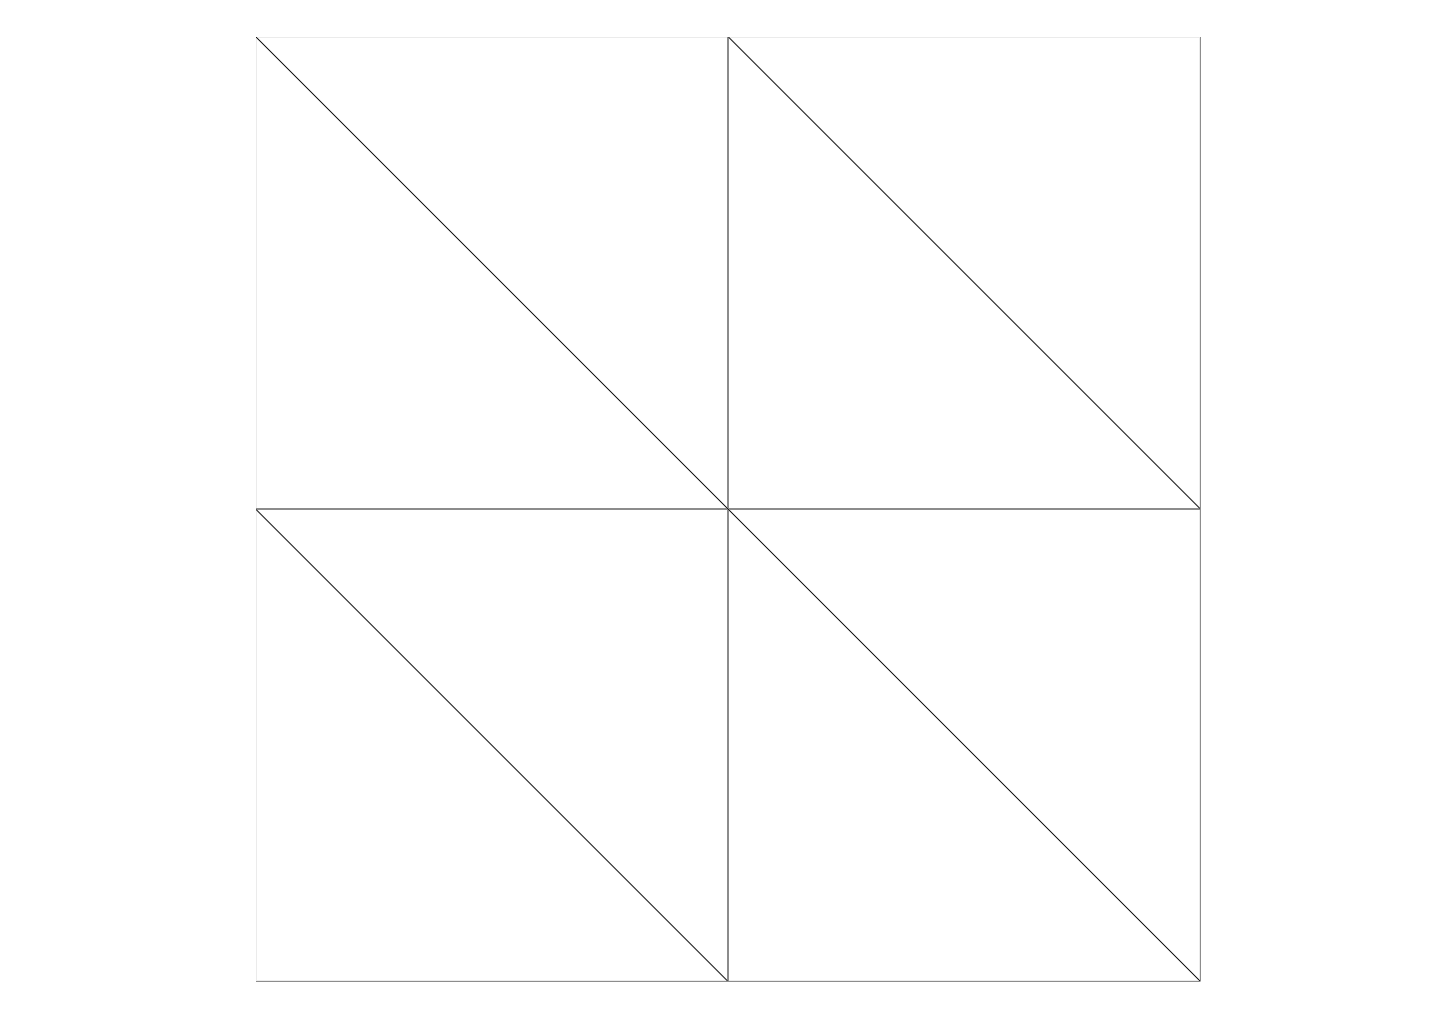
\includegraphics[width=1.0\linewidth,height=0.32\textheight,keepaspectratio]{data/synthetic_meshes/square_tesselation_2tri_Dirac_delta_1_v9_f8_wireframe.png}
		\caption{Sq2 v9\_f8 wireframe}\label{fig:sq2.a}
	\end{subfigure}
	\begin{subfigure}[b]{0.48\linewidth}
		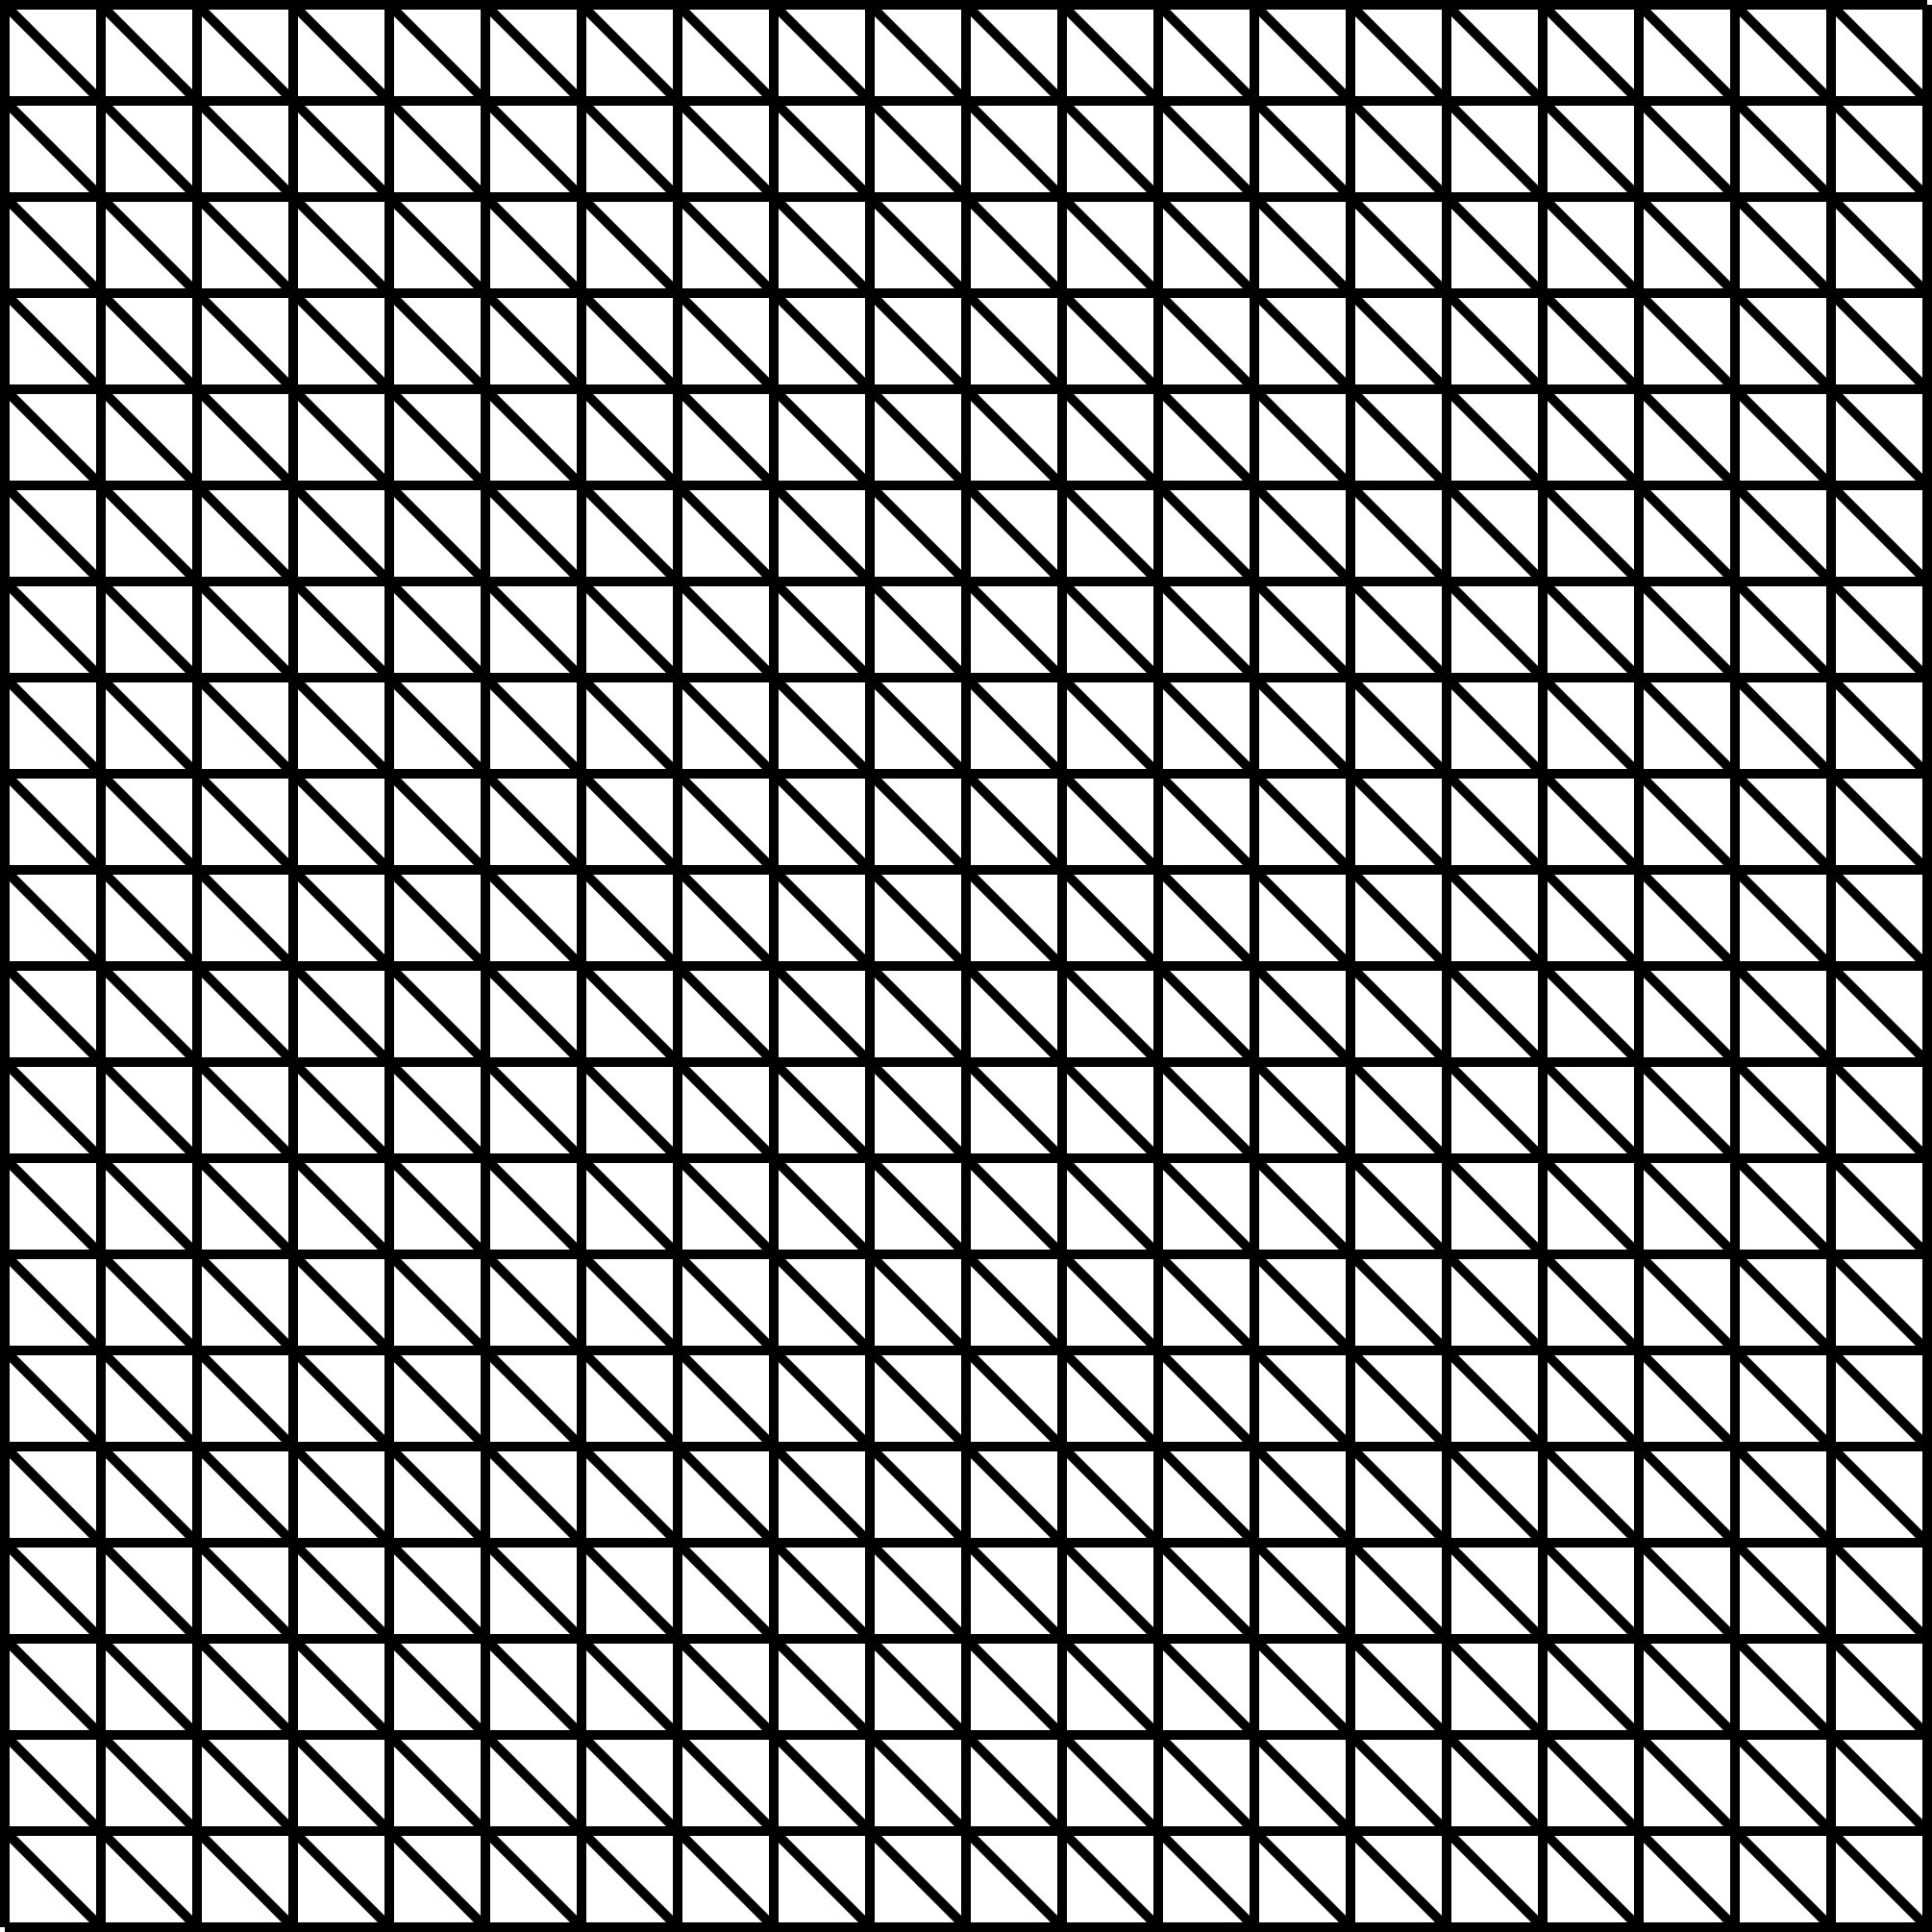
\includegraphics[width=1.0\linewidth,height=0.32\textheight,keepaspectratio]{data/synthetic_meshes/square_tesselation_2tri_Dirac_delta_10_v441_f800_wireframe.png}
		\caption{Sq2 v441\_f800 wireframe}\label{fig:sq2.b}
	\end{subfigure}

	\bigskip
	\begin{subfigure}[b]{0.48\linewidth}
		
\includegraphics[width=1.0\linewidth,height=0.32\textheight,keepaspectratio]{data/synthetic_meshes/square_tesselation_2tri_Dirac_delta_1_v9_f8_funcvals_0iter_crop.png}
		\caption{Sq2 v9\_f8 iter 0}\label{fig:sq2.c}
	\end{subfigure}
	\begin{subfigure}[b]{0.48\linewidth}
		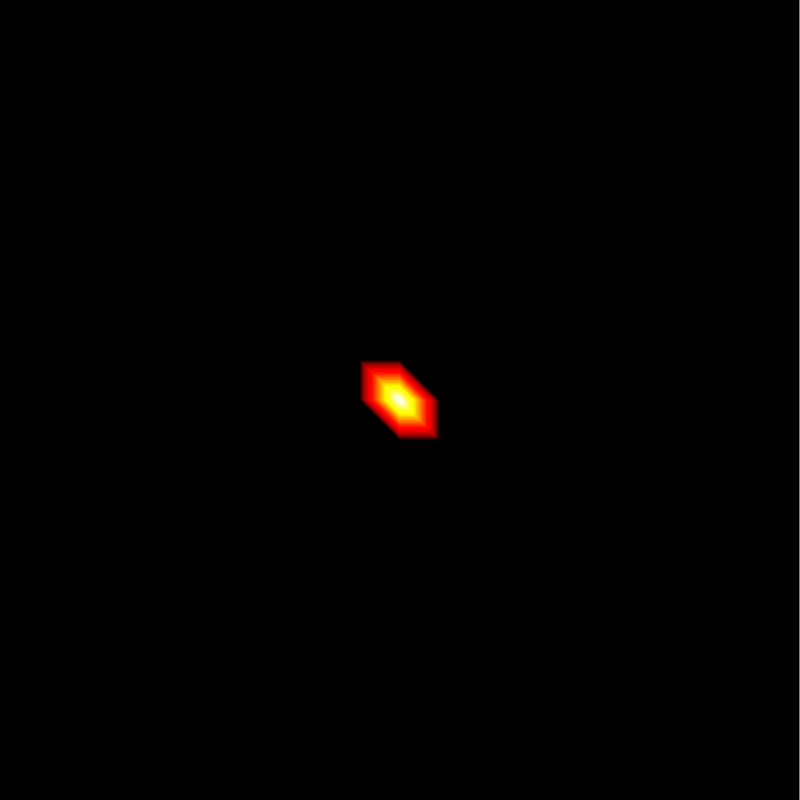
\includegraphics[width=1.0\linewidth,height=0.32\textheight,keepaspectratio]{data/synthetic_meshes/square_tessellation_2tri_Dirac_delta_10_v441_f800_funcvals_0iter.png}
		\caption{Sq2 v441\_f800 iter 0}\label{fig:sq2.d}
	\end{subfigure}

	\bigskip
	\begin{subfigure}[b]{0.48\linewidth}
		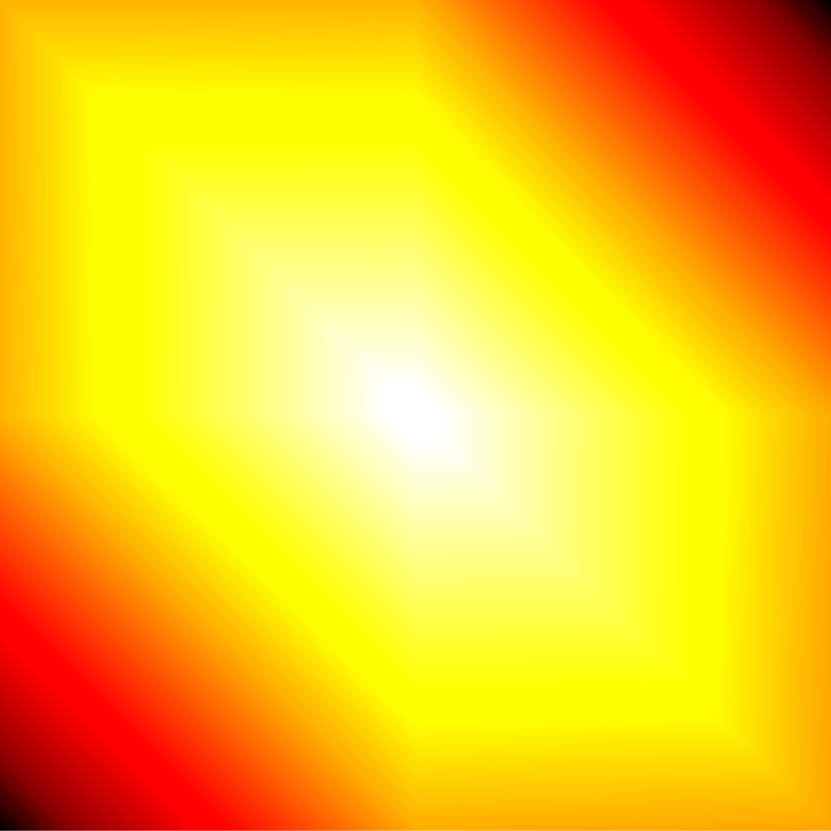
\includegraphics[width=1.0\linewidth,height=0.32\textheight,keepaspectratio]{data/synthetic_meshes/square_tesselation_2tri_Dirac_delta_1_v9_f8_funcvals_1iter_crop.png}
		\caption{Sq2 v9\_f8 iter 1}\label{fig:sq2.e}
	\end{subfigure}
	\begin{subfigure}[b]{0.48\linewidth}
		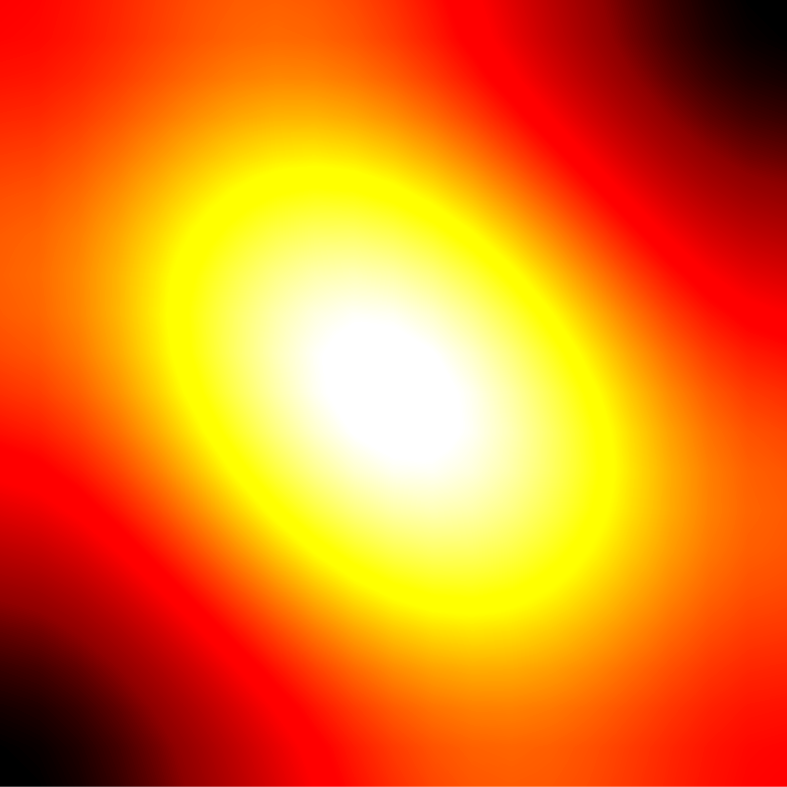
\includegraphics[width=1.0\linewidth,height=0.32\textheight,keepaspectratio]{data/synthetic_meshes/square_tessellation_2tri_Dirac_delta_10_v441_f800_funcvals_100iter.png}
		\caption{Sq2 v441\_f800 iter 100}\label{fig:sq2.f}
	\end{subfigure}}
	{\caption[Synthetic Square, 2 triangles, Dirac delta function]{A synthetic square, subdivided by triangles, with a Dirac delta function applied: (a) wireframe (b) colored by function value before filter (c) colored by function value after 1000 iterations
%GigaMesh~\cite{Mara10} with function values colored with the Improved Hot colorramp, exported as png after disabling the background grid [f7], maximizing the window, disabling screenshot cropping, as well as rejecting tiled rendering, finally cropping to content in GIMP.
	}\label{fig:sq2}}
\end{figure}
\todoCitation{}
\todoResearch{Why does sq2 10 need 100 iters to match sq 1 at 1 iters?}
\todoStyle{Why does sq2 1 iters 0 get differnt spacing?}
\todoStyle{Adjusting height, shrinks width => images no longer centered in their columns}

\subsubsection{Square grid, four triangles}

\subsubsection{Hexagonal grid}
\begin{figure}[ht]
\ffigbox
	{\begin{subfigure}[b]{0.48\linewidth}
		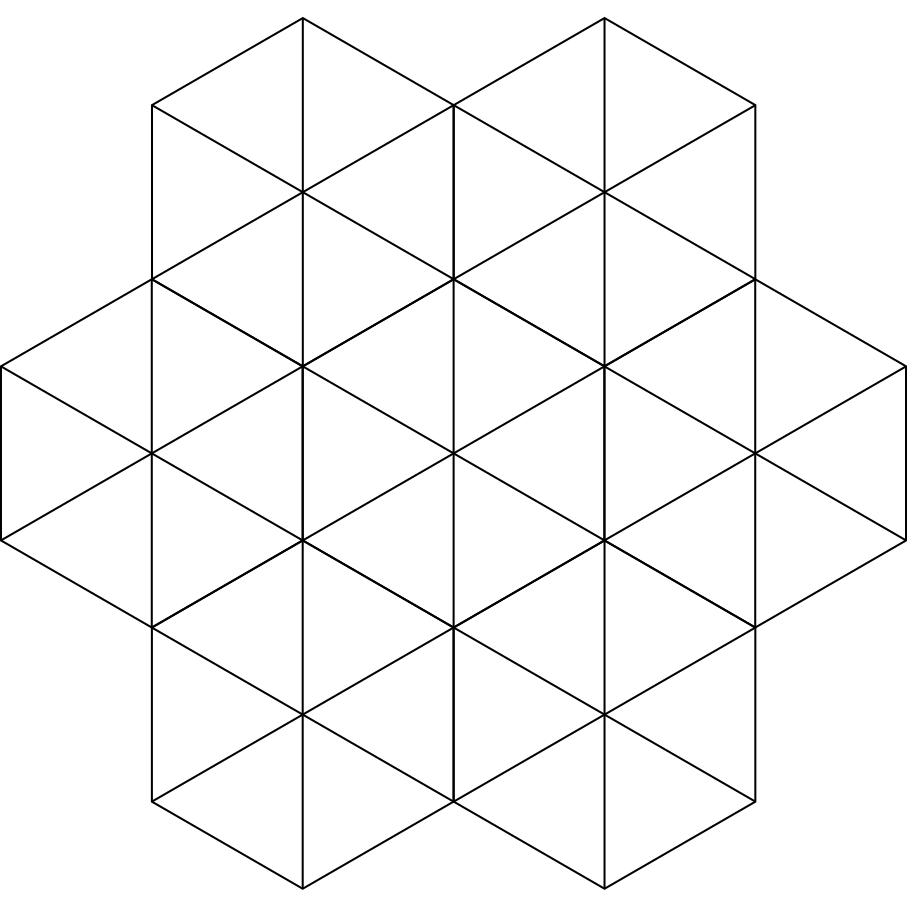
\includegraphics[width=1.0\linewidth,height=0.3\textheight,keepaspectratio]{data/synthetic_meshes/hexagonal_tessellation_Dirac_delta_1_v31_f42_wireframe.png}
		\caption{Hex v31\_f42 wireframe}\label{fig:hex.a}
	\end{subfigure}
	\begin{subfigure}[b]{0.48\linewidth}
		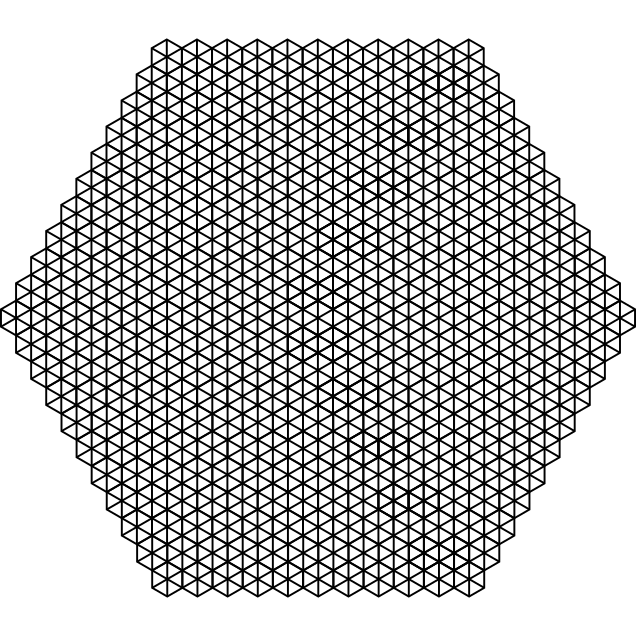
\includegraphics[width=1.0\linewidth,height=0.3\textheight,keepaspectratio]{data/synthetic_meshes/hexagonal_tessellation_Dirac_delta_10_v1057_f1986_wireframe.png}
		\caption{Hex v1057\_f1986 wireframe}\label{fig:hex.b}
	\end{subfigure}

	\bigskip
	\begin{subfigure}[b]{0.48\linewidth}
		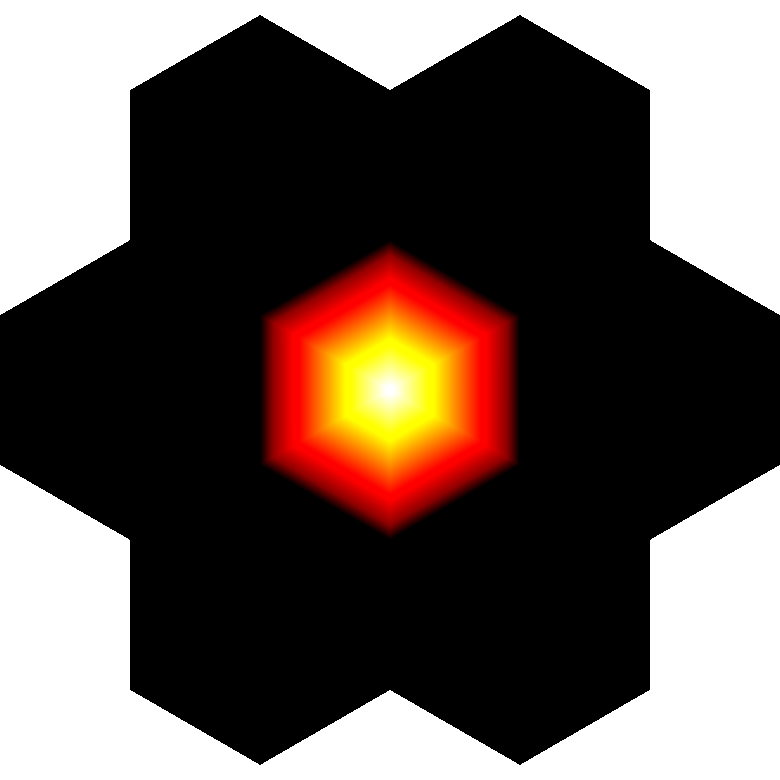
\includegraphics[width=1.0\linewidth,height=0.3\textheight,keepaspectratio]{data/synthetic_meshes/hexagonal_tessellation_Dirac_delta_1_v31_f42_funcvals_0iter_crop.png}
		\caption{Hex v31\_f42 iter 0}\label{fig:hex.c}
	\end{subfigure}
	\begin{subfigure}[b]{0.48\linewidth}
		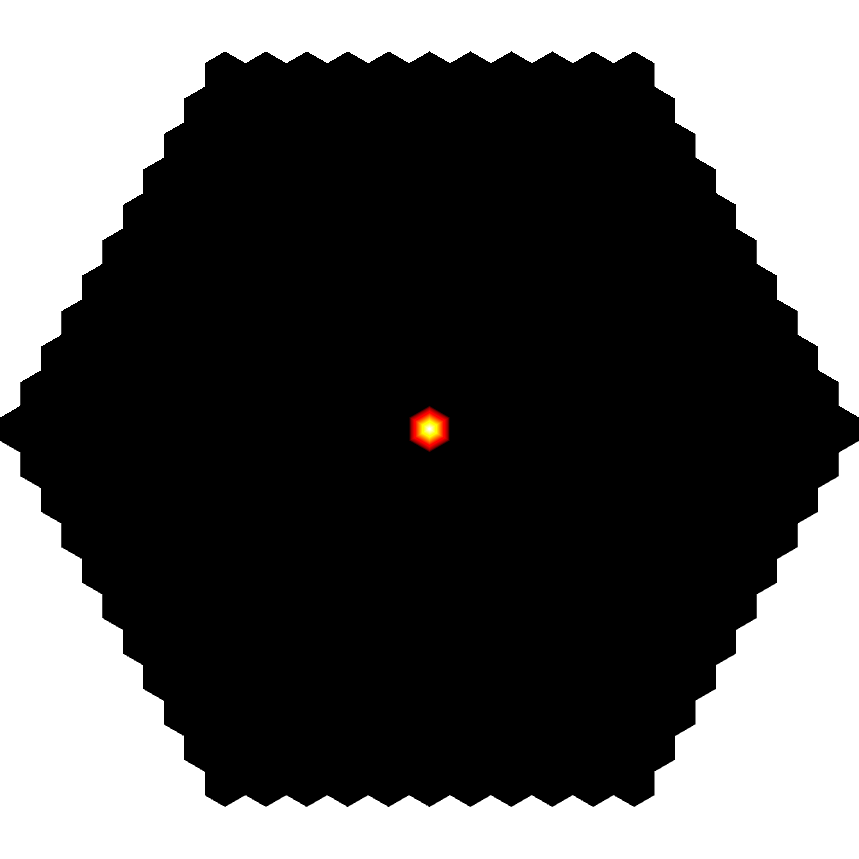
\includegraphics[width=1.0\linewidth,height=0.3\textheight,keepaspectratio]{data/synthetic_meshes/hexagonal_tessellation_Dirac_delta_10_v1057_f1986_funcvals_0iter_crop.png}
		\caption{Hex v1057\_f1986 iter 0}\label{fig:hex.d}
	\end{subfigure}

	\bigskip
	\begin{subfigure}[b]{0.48\linewidth}
		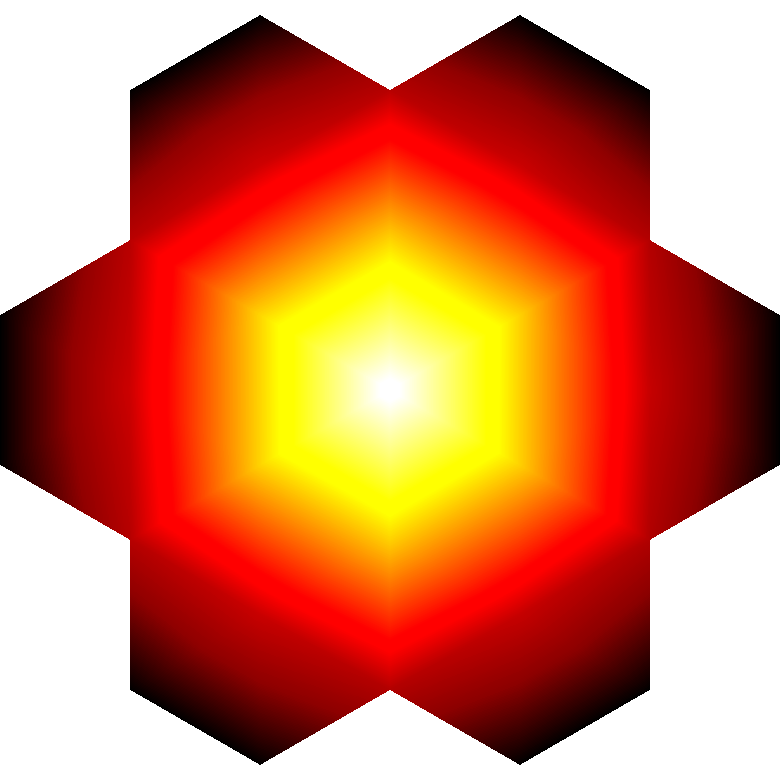
\includegraphics[width=1.0\linewidth,height=0.3\textheight,keepaspectratio]{data/synthetic_meshes/hexagonal_tessellation_Dirac_delta_1_v31_f42_funcvals_2iter_crop.png}
		\caption{Hex v31\_f42 iter 2}\label{fig:hex.e}
	\end{subfigure}
	\begin{subfigure}[b]{0.48\linewidth}
		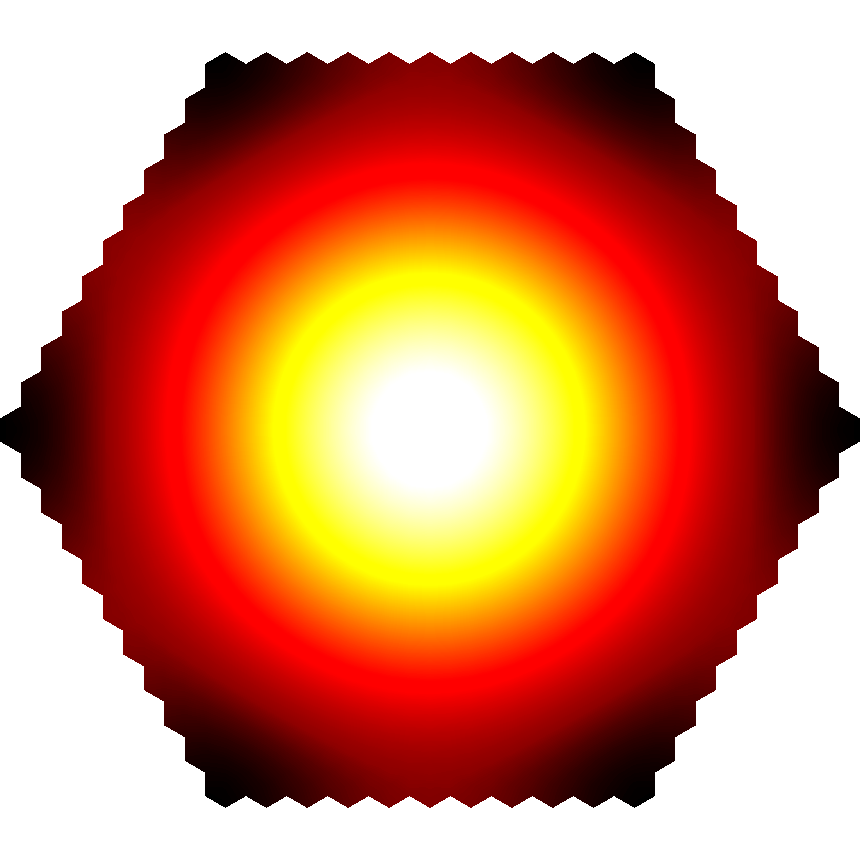
\includegraphics[width=1.0\linewidth,height=0.3\textheight,keepaspectratio]{data/synthetic_meshes/hexagonal_tessellation_Dirac_delta_10_v1057_f1986_funcvals_200iter_crop.png}
		\caption{Hex v1057\_f1986 iter 200}\label{fig:hex.f}
	\end{subfigure}}
	{\caption[Synthetic Hexagonal Tessellations, Dirac delta function]{A synthetic hexagonal tessellation, subdivided by triangles, with a Dirac delta function applied: (a) v31 f42 wireframe (b) v1057 f1986 wireframe (c) v31 f42 colored by function value before filter (d) v1057 f1986 colored by function value before filter (e) v31 f42 colored by function value after 2 iterations (e) v1057 f1986 colored by function value after 200 iterations.
% All using the colorramp "Hot (improved)"~\cite[p.~???]{Brewer2003}~\cite[p.~19]{Giga17}, visualized using GigaMesh~\cite{Mara10}, exported as png after disabling the background grid [f7], maximizing the window, disabling screenshot cropping, as well as rejecting tiled rendering, finally cropping to content in GIMP.
	}\label{fig:hex}}
\end{figure}
\todoCitation{}

\subsubsection{Random vertices within a circle}
\begin{figure}[ht]
\ffigbox
	{\begin{subfigure}[b]{0.48\linewidth}
		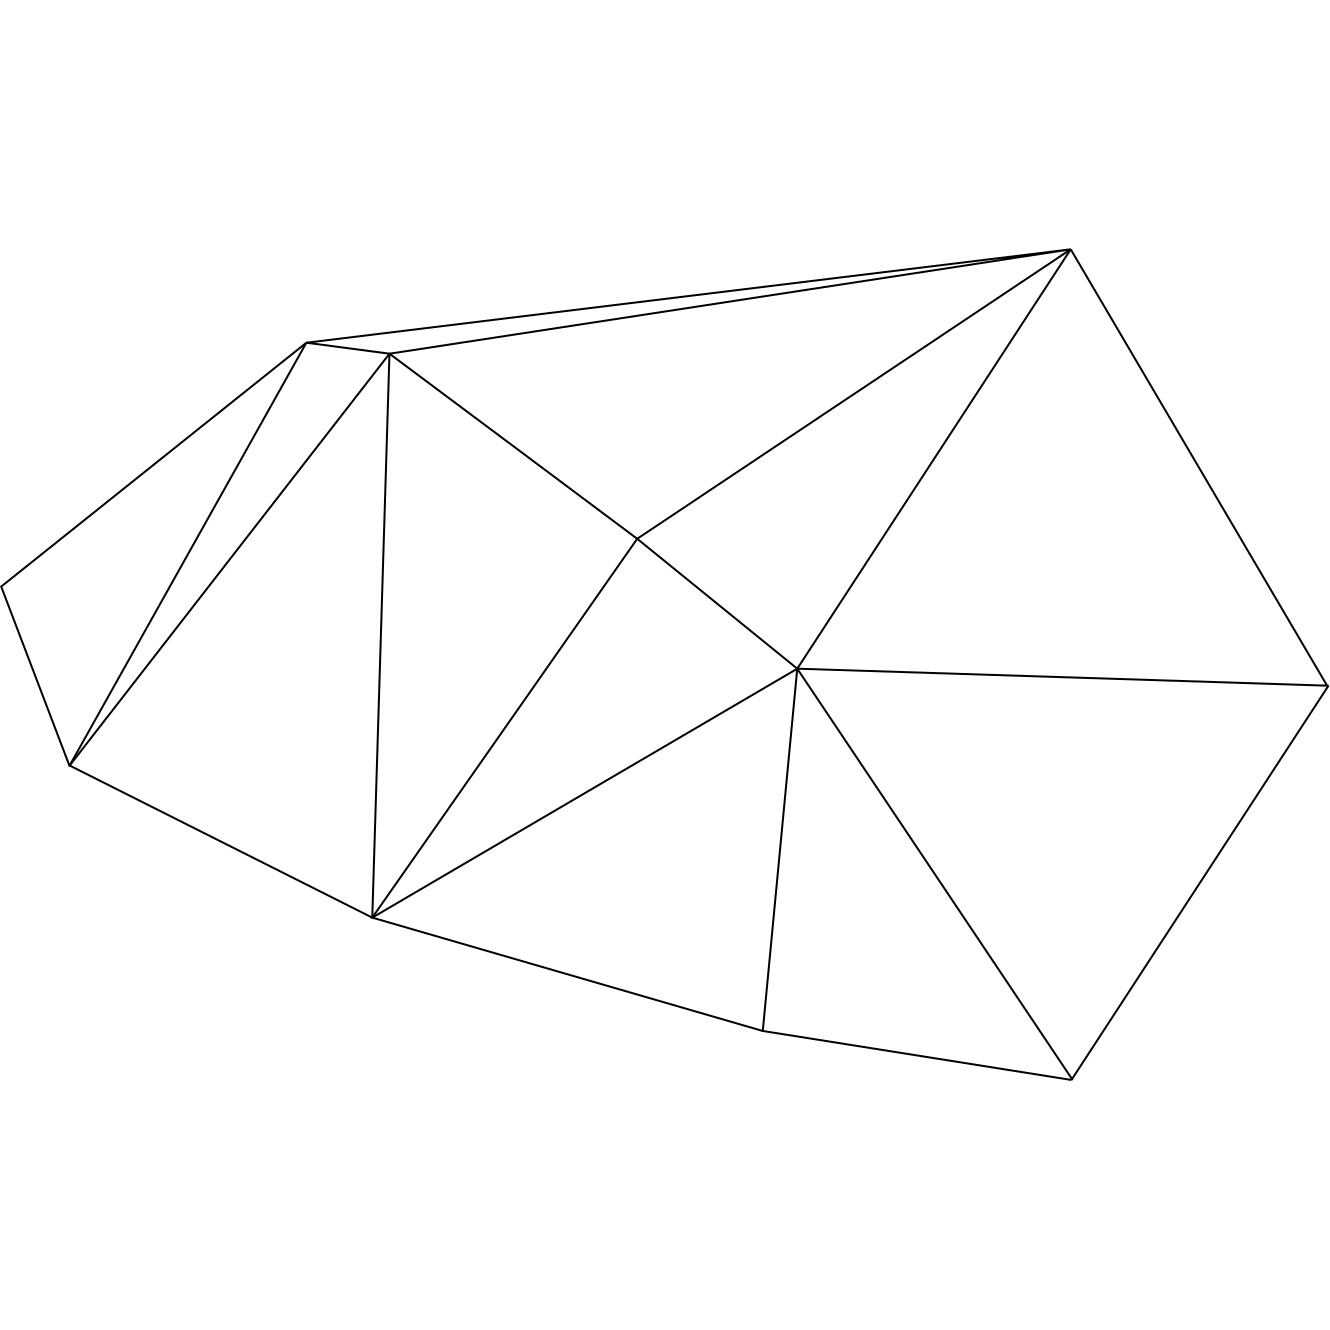
\includegraphics[width=1.0\linewidth,height=0.3\textheight,keepaspectratio]{data/synthetic_meshes/random_circle_tessellation_Dirac_delta_1_v11_f12_wireframe.png}
		\caption{R.Circ v11\_f12 wireframe}\label{fig:rcirc.a}
	\end{subfigure}
	\begin{subfigure}[b]{0.48\linewidth}
		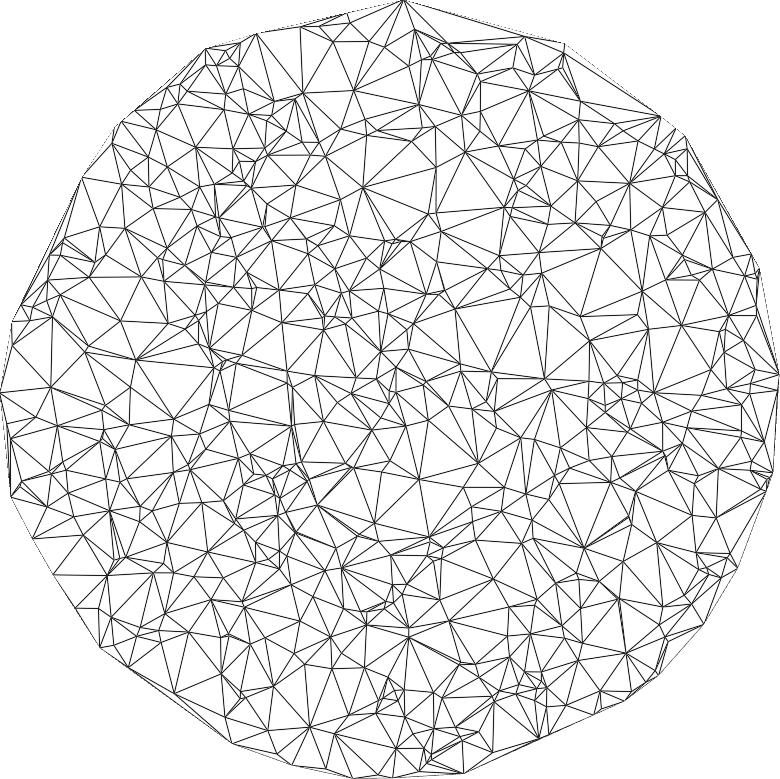
\includegraphics[width=1.0\linewidth,height=0.3\textheight,keepaspectratio]{data/synthetic_meshes/random_circle_tessellation_Dirac_delta_10_v641_f1252_wireframe.png}
		\caption{R.Circ v641\_f1252 wireframe}\label{fig:rcirc.b}
	\end{subfigure}

	\bigskip
	\begin{subfigure}[b]{0.48\linewidth}
		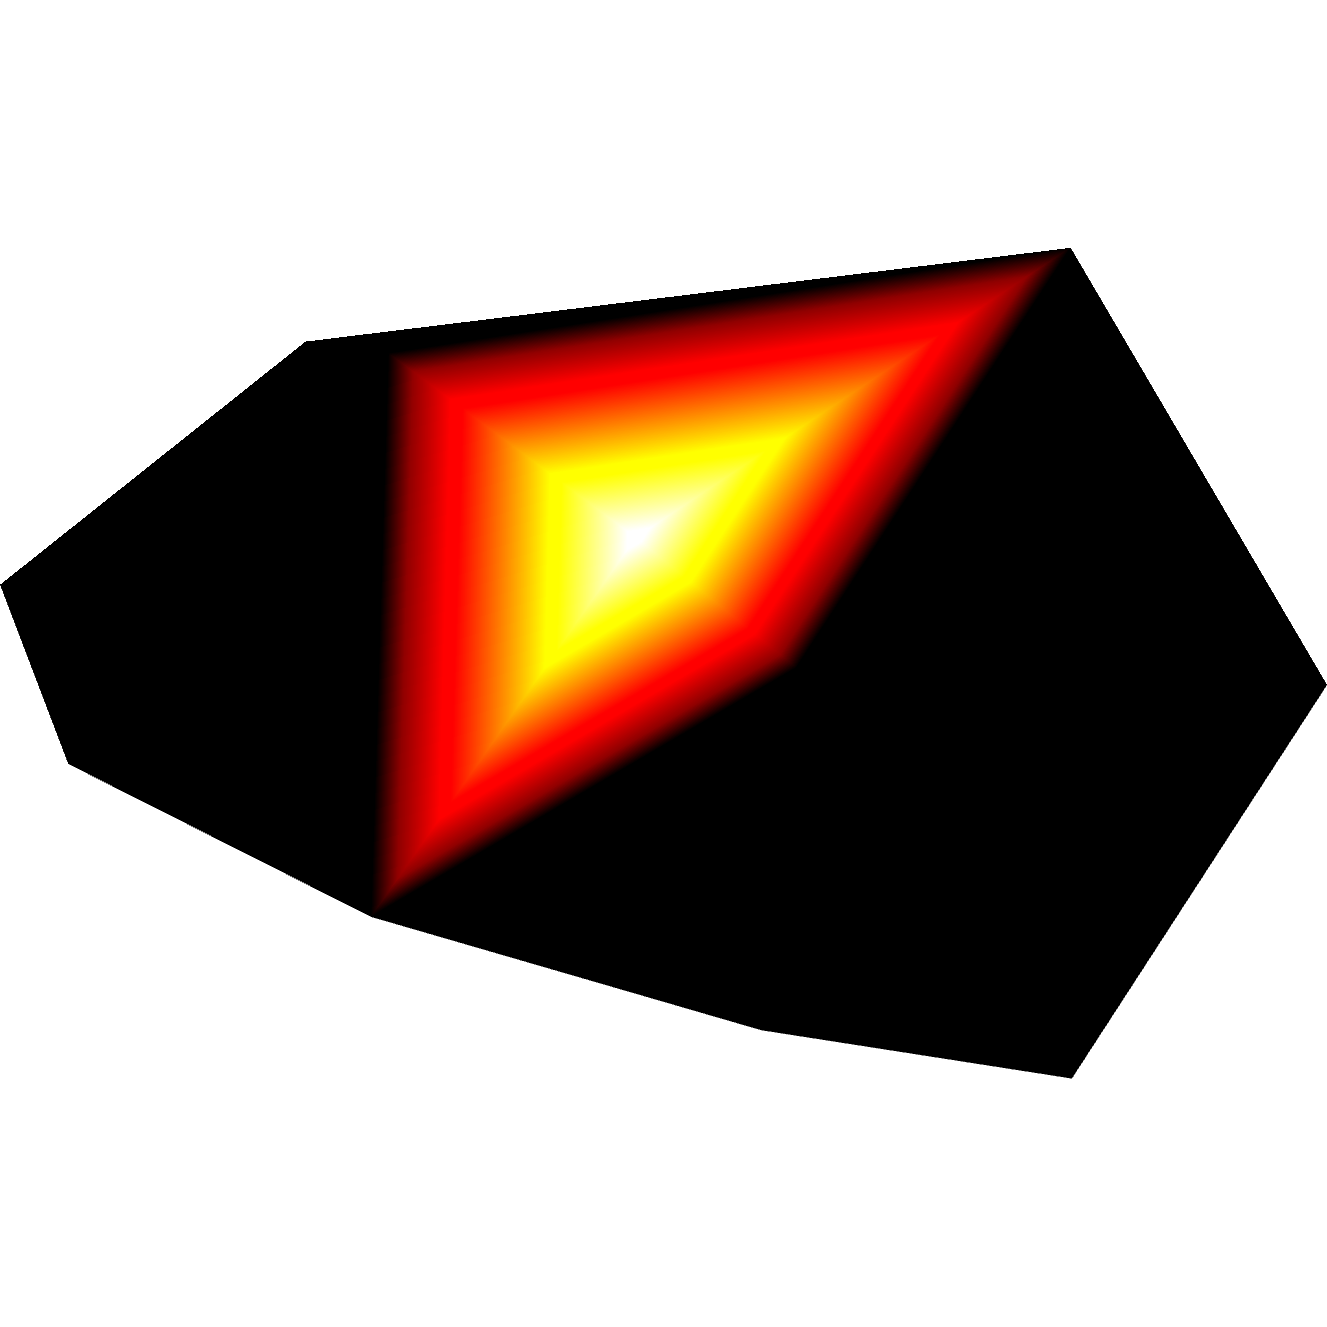
\includegraphics[width=1.0\linewidth,height=0.3\textheight,keepaspectratio]{data/synthetic_meshes/random_circle_tessellation_Dirac_delta_1_v11_f12_funcvals_0iter.png}
		\caption{R.Circ v11\_f12 iter 0}\label{fig:rcirc.c}
	\end{subfigure}
	\begin{subfigure}[b]{0.48\linewidth}
		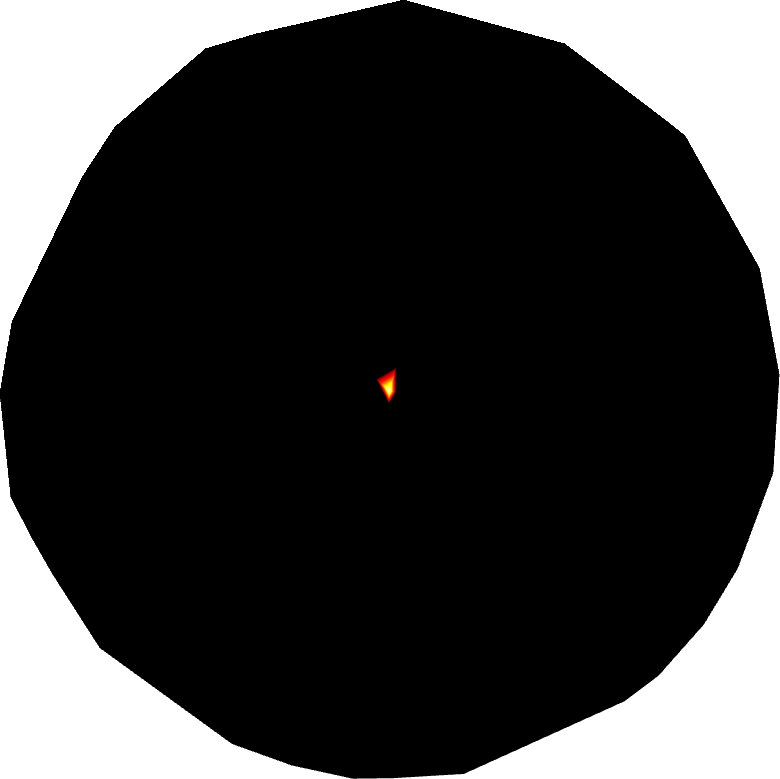
\includegraphics[width=1.0\linewidth,height=0.3\textheight,keepaspectratio]{data/synthetic_meshes/random_circle_tessellation_Dirac_delta_10_v641_f1252_funcvals_0iter.png}
		\caption{R.Circ v641\_f1252 iter 0}\label{fig:rcirc.d}
	\end{subfigure}

	\bigskip
	\begin{subfigure}[b]{0.48\linewidth}
		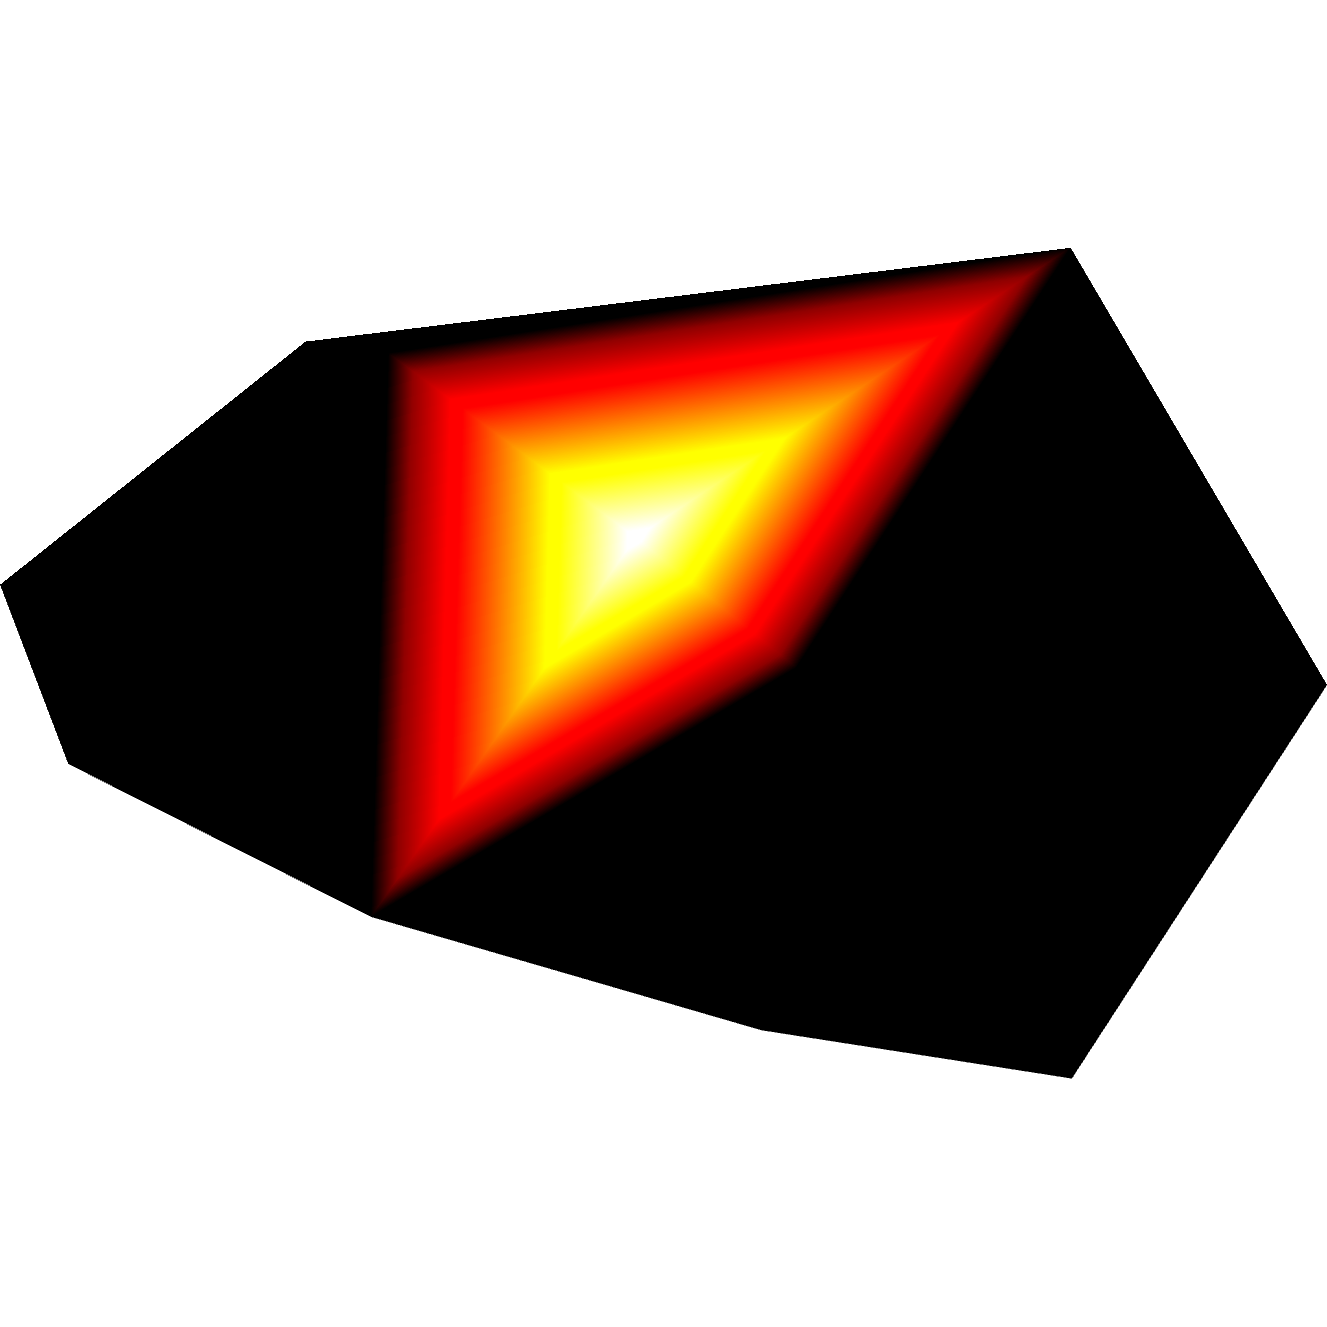
\includegraphics[width=1.0\linewidth,height=0.3\textheight,keepaspectratio,height=0.3\textheight,keepaspectratio]{data/synthetic_meshes/random_circle_tessellation_Dirac_delta_1_v11_f12_funcvals_0iter.png}
		\caption{R.Circ v11\_f12 iter 2}\label{fig:rcirc.e}
	\end{subfigure}
	\begin{subfigure}[b]{0.48\linewidth}
		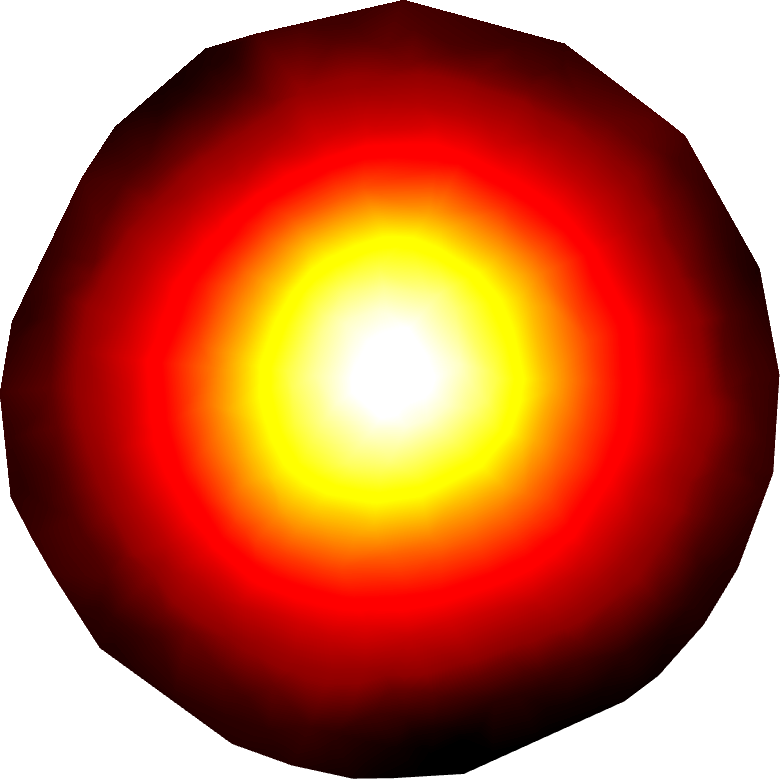
\includegraphics[width=1.0\linewidth,height=0.3\textheight,keepaspectratio,height=0.3\textheight,keepaspectratio]{data/synthetic_meshes/random_circle_tessellation_Dirac_delta_10_v641_f1252_funcvals_10000iter.png}
		\caption{R.Circ v641\_f1252 iter 10,000}\label{fig:rcirc.f}
	\end{subfigure}}
	{\caption[Synthetic random vertices equally distributed per radius, Dirac delta function]{A synthetic circle filled with random vertices equaly distributed per radius, triangulated by Delauney method~\cite[p.~??]{todoCitation}, with a Dirac delta function applied: (a) v11\_f12 wireframe (b) v641\_f1252 wireframe (c) v11\_f12 colored by function value before filter (d) v641\_f1252 colored by function value before filter (e) v11\_f12 colored by function value after 2 iterations (f) v641\_f1252 colored by function value after 10,000 iterations.
%All using the colorramp "Hot (improved)"~\cite[p.~???]{Brewer2003}~\cite[p.~19]{Giga17}, visualized using GigaMesh~\cite{Mara10}, exported as png after disabling the background grid [f7], maximizing the window, disabling screenshot cropping, as well as rejecting tiled rendering, finally cropping to content in GIMP.
}\label{fig:rcirc}}
\end{figure}
\todoCitation{}
\todoResearch{Why and who equally distributed}

%\subsection{Debossed H}
%In Figure \ref{fig:h}, we show a debossed capital letter H.\footnote{The H is
%as a nod to Heidelberg University and the cuniform script studied by the FCGL.}
%\begin{figure}[ht]
%\centering
%	\begin{subfigure}{.48\linewidth}
%		\centering
%		\resizebox{0.48\linewidth}{!}{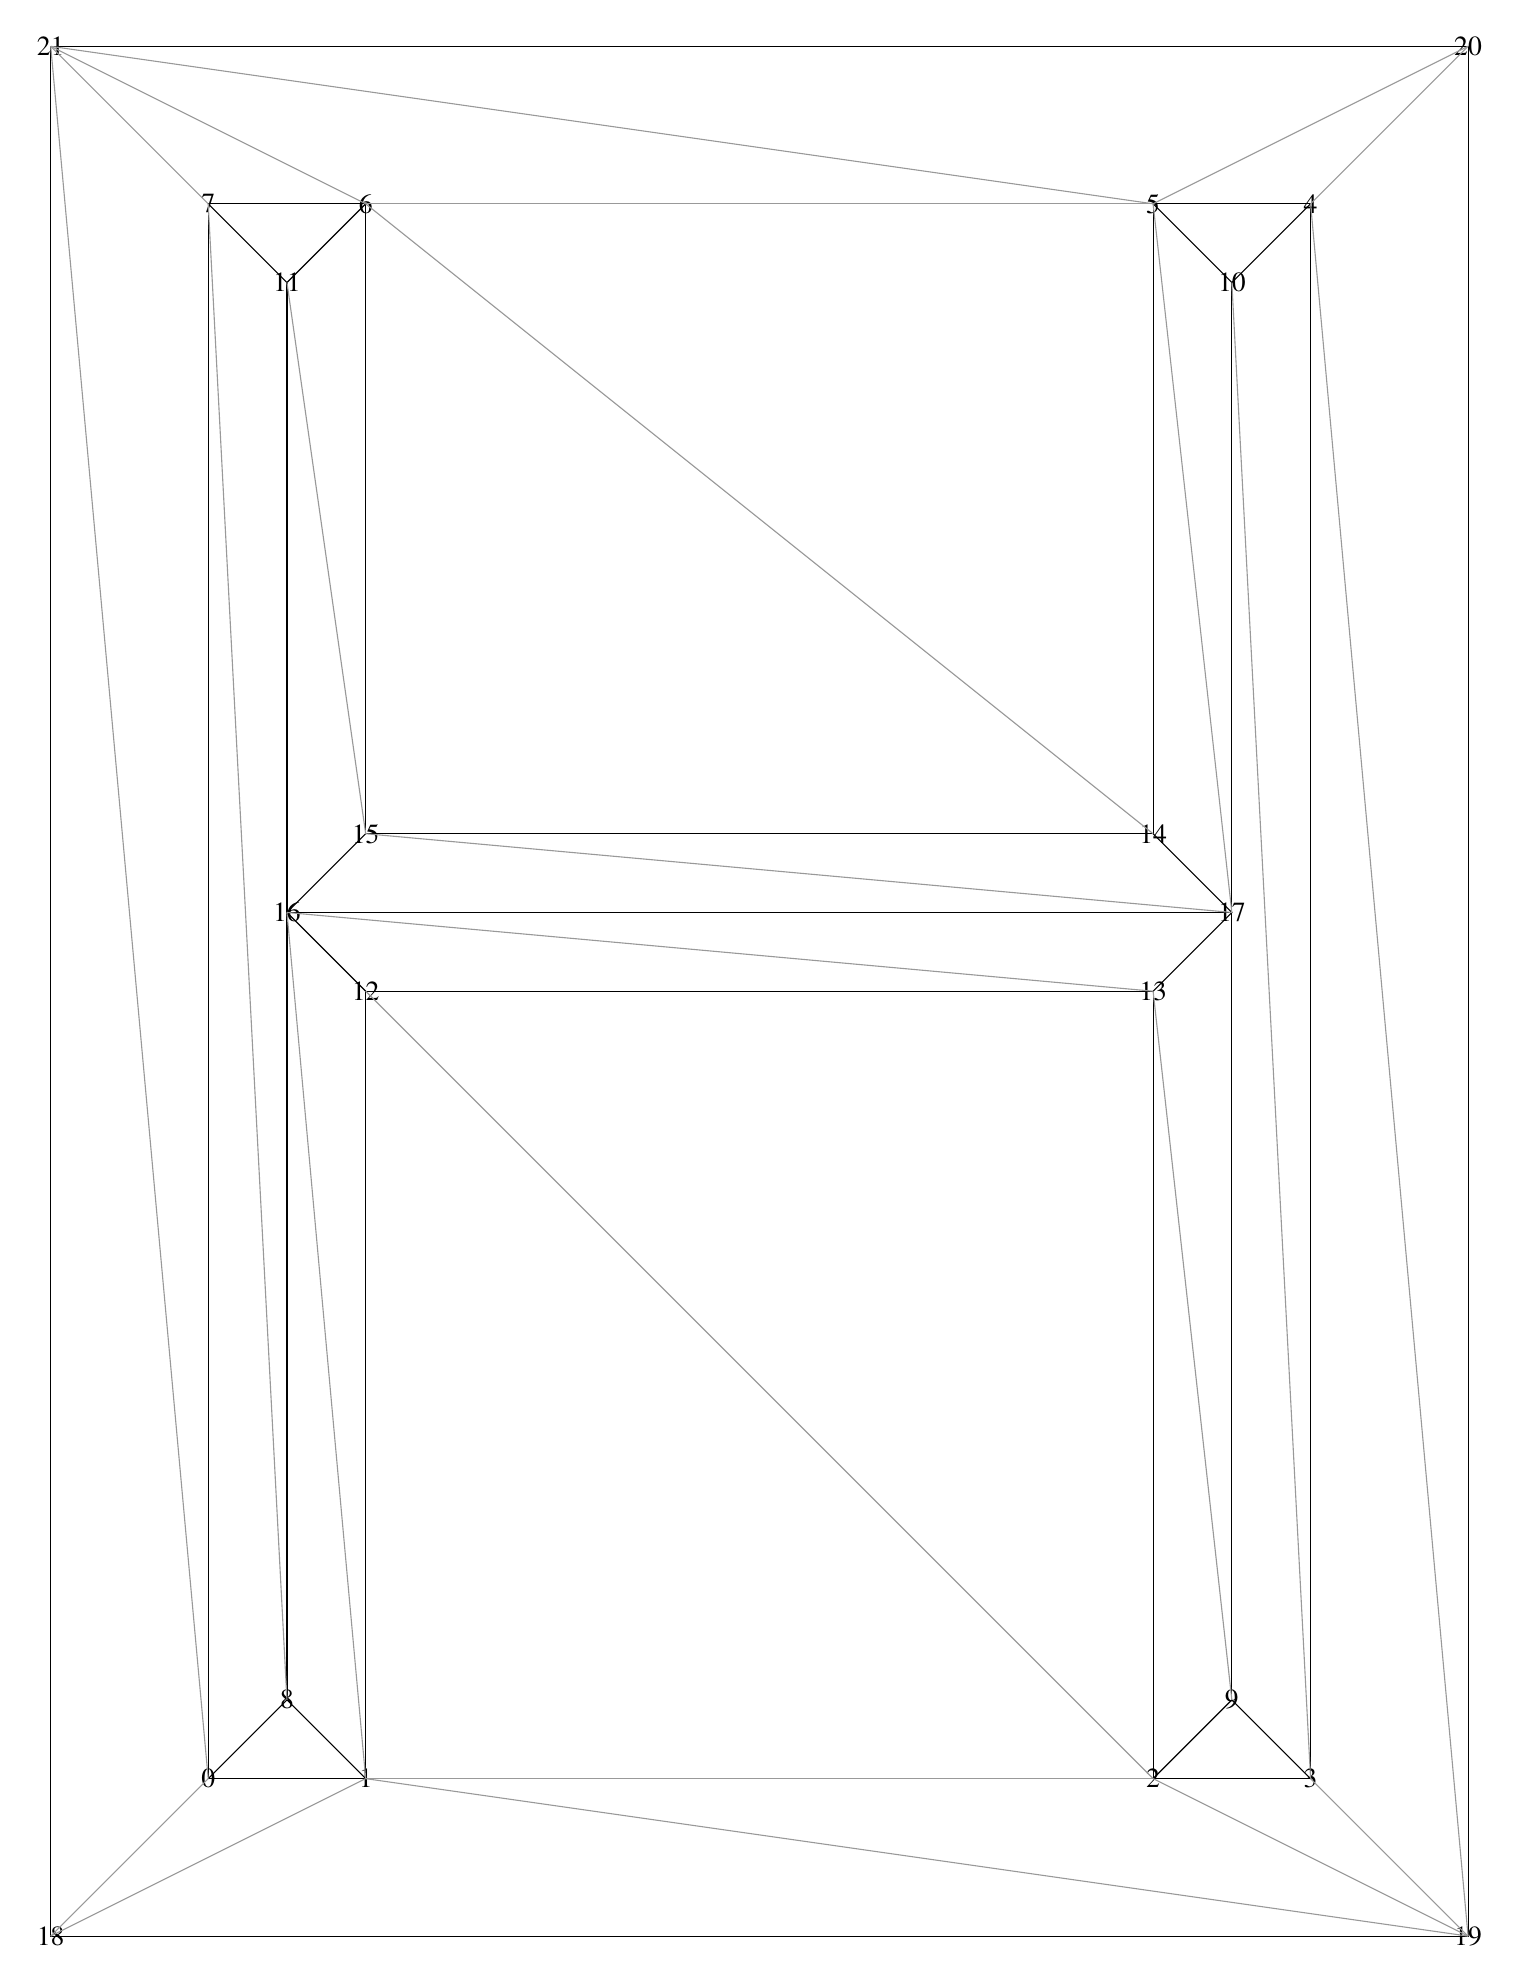
\begin{tikzpicture}
% Colors
\definecolor{outlineColor}{RGB}{0,0,0}
\definecolor{supportColor}{RGB}{153,153,153}
% Main H shape and Outline
\begin{scope}[outlineColor]
	\draw( 0, 0) node  {0} % 0
	  -- ( 2, 0) node  {1} % 1
	  -- ( 2,10) node {12} %12
	  -- (12,10) node {13} %13
	  -- (12, 0) node  {2} % 2
	  -- (14, 0) node  {3} % 3
	  -- (14,20) node  {4} % 4
	  -- (12,20) node  {5} % 5
	  -- (12,12) node {14} %14
	  -- ( 2,12) node {15} %15
	  -- ( 2,20) node  {6} % 6
	  -- ( 0,20) node  {7} % 7
	  -- cycle;  
	\draw( 0, 0) % 0
	  -- ( 1, 1) node  {8} % 8
	  -- ( 2, 0);% 1
	\draw(12, 0) % 2
	  -- (13, 1) node  {9} % 9
	  -- (14, 0);% 3
	\draw(14,20) % 4
	  -- (13,19) node {10} %10
	  -- (12,20);% 5
	\draw( 2,20) % 6
	  -- ( 1,19) node {11} %11
	  -- ( 0,20);% 7
	\draw( 2,10) %12
	  -- ( 1,11) node {16} %16
	  -- ( 2,12);%15
	\draw(12,10) %13
	  -- (13,11) node {17} %17
	  -- (12,12);%14
	\draw( 1, 1) % 8
	  -- ( 1,19);%11
	\draw(13, 1) % 9
	  -- (13,19);%10
	\draw( 1,11) %16
	  -- (13,11);%17
	\draw(-2,-2) node {18} %18
	  -- (16,-2) node {19} %19
	  -- (16,22) node {20} %20
	  -- (-2,22) node {21} %21
	  -- cycle;
\end{scope}
\begin{scope}[supportColor, thin]
	\draw( 0, 0) -- (-2,-2); % 0--18
	\draw( 0, 0) -- (-2,22); % 0--21
	\draw( 2, 0) -- (12, 0); % 1-- 2
	\draw( 2, 0) -- ( 1,11); % 1--16
	\draw( 2, 0) -- (-2,-2); % 1--18
	\draw( 2, 0) -- (16,-2); % 1--19
	\draw(12, 0) -- ( 2,10); % 2--12
	\draw(12, 0) -- (16,-2); % 2--19
	\draw(14, 0) -- (13,19); % 3--10
	\draw(14, 0) -- (16,-2); % 3--19
	\draw(14,20) -- (16,-2); % 4--19
	\draw(14,20) -- (16,22); % 4--20
	\draw(12,20) -- ( 2,20); % 5-- 6
	\draw(12,20) -- (13,11); % 5--17
	\draw(12,20) -- (16,22); % 5--20
	\draw(12,20) -- (-2,22); % 5--21
	\draw( 2,20) -- (12,12); % 6--14
	\draw( 2,20) -- (-2,22); % 6--21
	\draw( 0,20) -- ( 1, 1); % 7-- 8
	\draw( 0,20) -- (-2,22); % 7--21
	\draw(13, 1) -- (12,10); % 9--13
	\draw( 1,19) -- ( 2,12); %11--15
	\draw(12,10) -- ( 1,11); %13--16
	\draw( 2,12) -- (13,11); %15--17
\end{scope}
\end{tikzpicture}
}
%		\caption{HWireframe}\label{fig:h.a}
%	\end{subfigure}
%	\hfill
%	\begin{subfigure}{.48\linewidth}
%		\centering
%		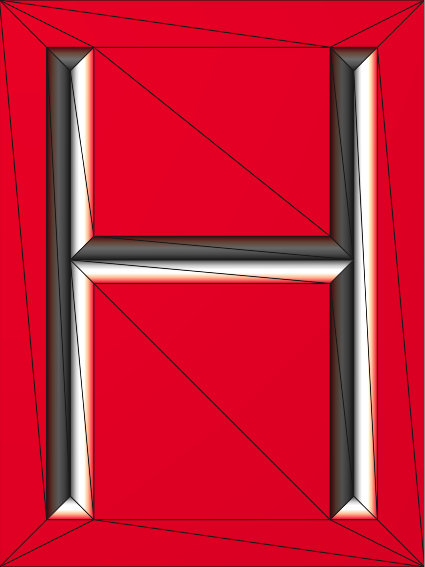
\includegraphics[width=0.48\linewidth]{data/synthetic_meshes/h_colored.png}
%		\caption{HColored}\label{fig:h.b}
%	\end{subfigure}
%	\caption[A debossed H, which contains 22 vertices and 36 faces.]{A debossed H,
%	which contains 22 vertices and 36 faces: (a) wireframe (b) colored by the
%	relation to its distance to an underlying plane, in RdGy
%	colorramp~\cite[p.~???]{Brewer2003}~\cite[p.~19]{Giga17}, visualized using the
%	GigaMesh~\cite{Mara10} framework with triangle edges rendered.}\label{fig:h}
%\end{figure}
To evaluate methods available for discrete surfaces, we can increase the number
of vertices of our synthetic wedge using five iterations of the mid-edge
subdivision scheme [PR97,
HW99].~\cite[p.~38]{Mara12}



\section{Acquired Data}
Acquired Data examples are actually recorded by sensors.
Something in Archaeology
Cuneiform Tablets
Mayan Tablets
Dynamic Earth models

\subsection{University Seal}
Unisiegel\_\- UAH\_\- Ebay-Siegel\_\- Uniarchiv\_\- HE2066-60\_\- 010614\_\- partial\_\- ASCII.ply
%\begin{figure}[ht]
%\ffigbox
%	{\begin{subfigure}[b]{0.48\linewidth}
%		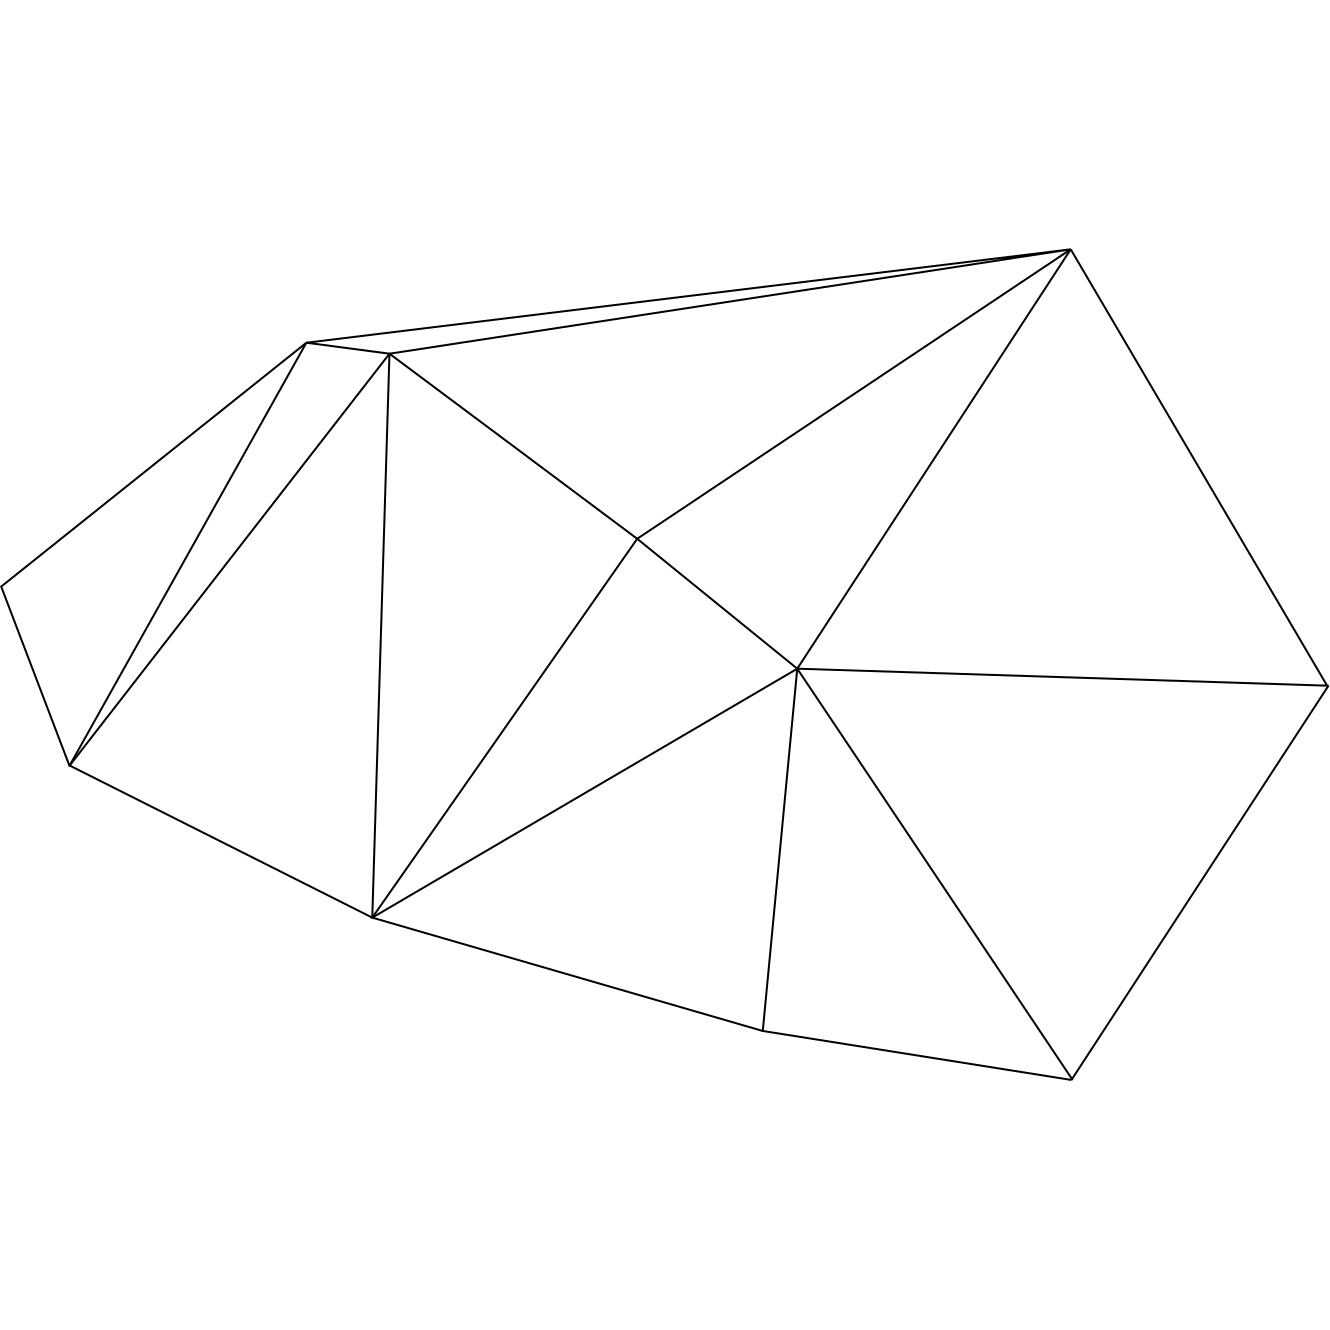
\includegraphics[width=1.0\linewidth,height=0.3\textheight,keepaspectratio]{data/synthetic_meshes/random_circle_tessellation_Dirac_delta_1_v11_f12_wireframe.png}
%		\caption{R.Circ v11\_f12 wireframe}\label{fig:rcirc.a}
%	\end{subfigure}
%	\begin{subfigure}[b]{0.48\linewidth}
%		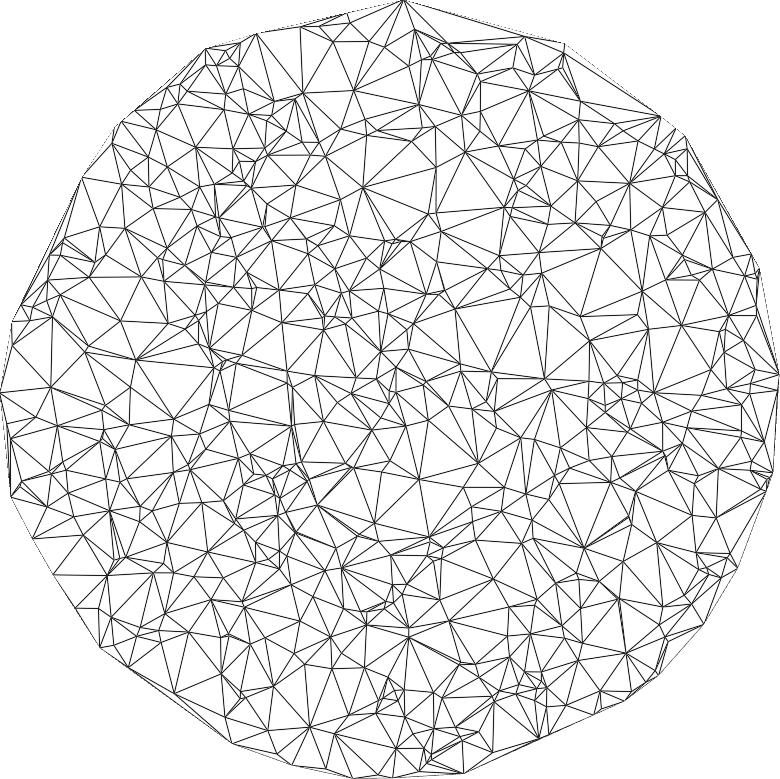
\includegraphics[width=1.0\linewidth,height=0.3\textheight,keepaspectratio]{data/synthetic_meshes/random_circle_tessellation_Dirac_delta_10_v641_f1252_wireframe.png}
%		\caption{R.Circ v641\_f1252 wireframe}\label{fig:rcirc.b}
%	\end{subfigure}
%
%	\bigskip
%	\begin{subfigure}[b]{0.48\linewidth}
%		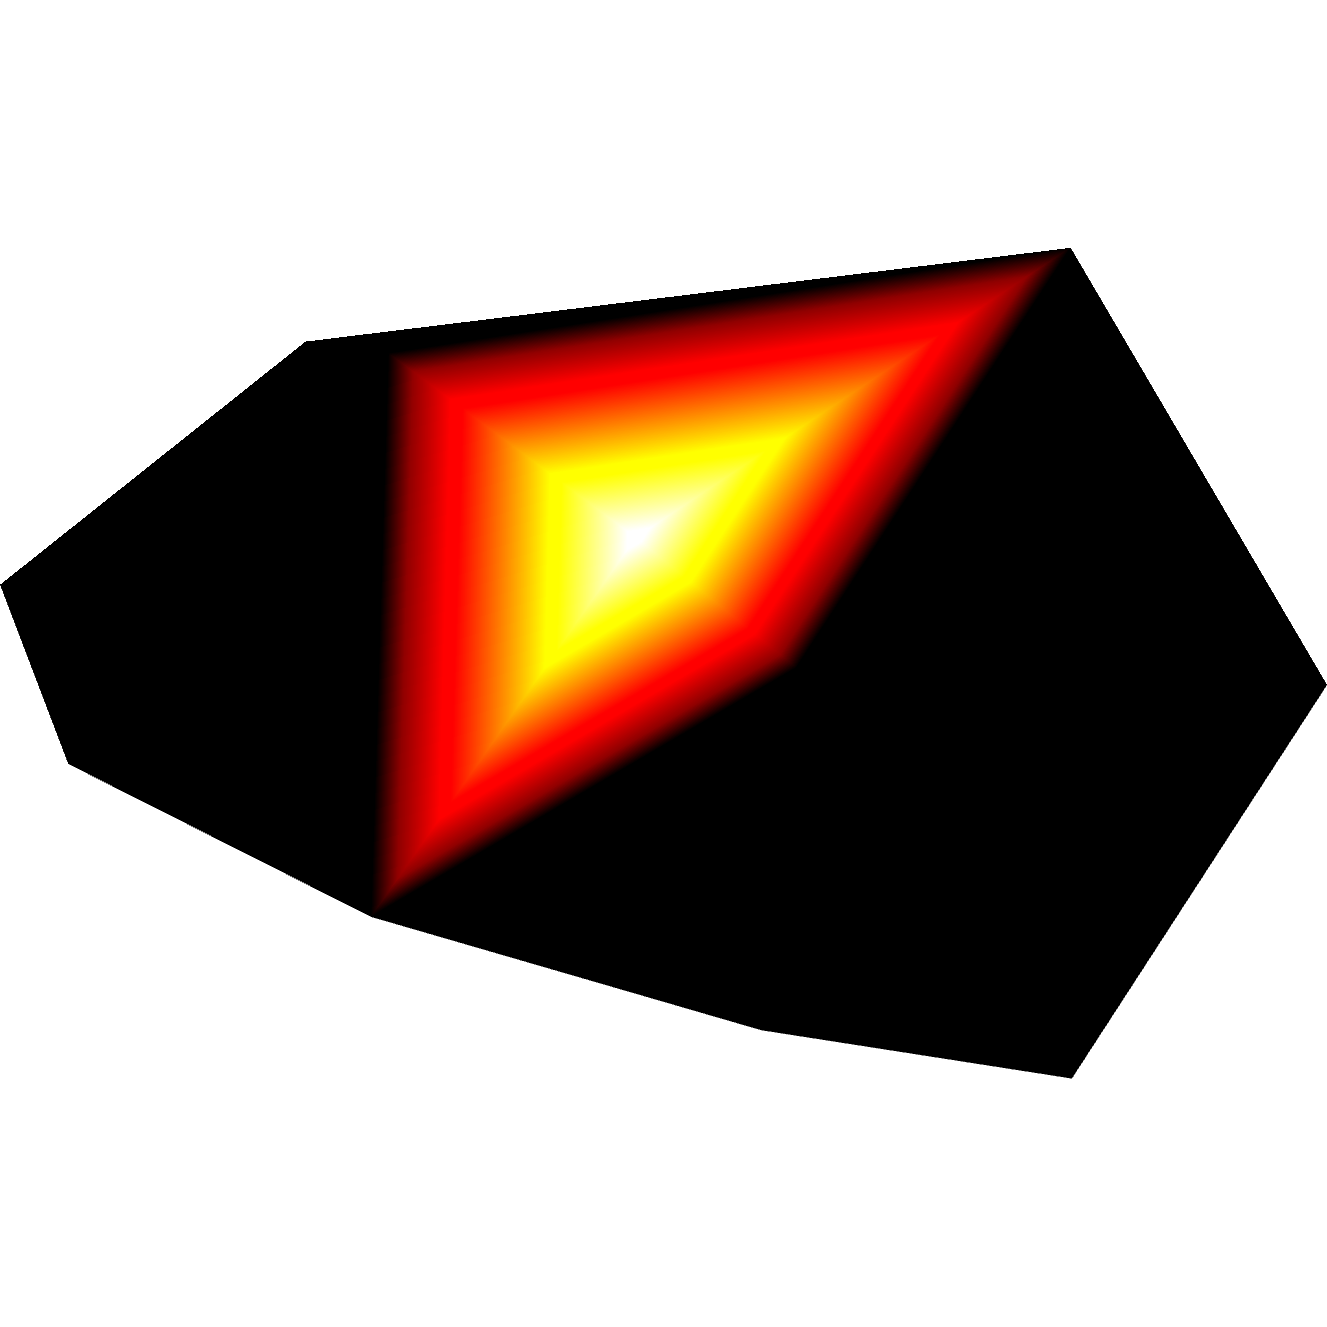
\includegraphics[width=1.0\linewidth,height=0.3\textheight,keepaspectratio]{data/synthetic_meshes/random_circle_tessellation_Dirac_delta_1_v11_f12_funcvals_0iter.png}
%		\caption{R.Circ v11\_f12 iter 0}\label{fig:rcirc.c}
%	\end{subfigure}
%	\begin{subfigure}[b]{0.48\linewidth}
%		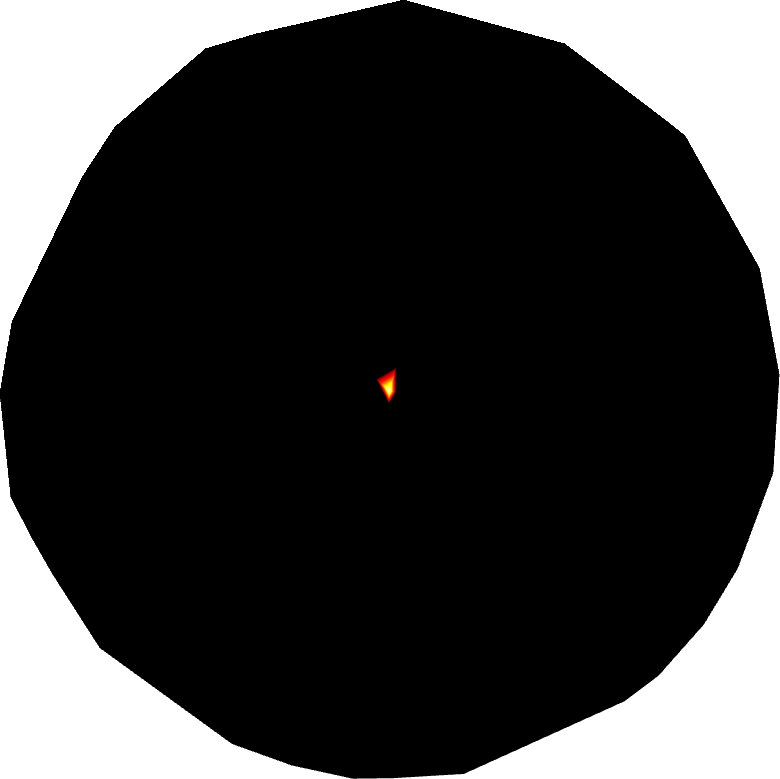
\includegraphics[width=1.0\linewidth,height=0.3\textheight,keepaspectratio]{data/synthetic_meshes/random_circle_tessellation_Dirac_delta_10_v641_f1252_funcvals_0iter.png}
%		\caption{R.Circ v641\_f1252 iter 0}\label{fig:rcirc.d}
%	\end{subfigure}
%
%	\bigskip
%	\begin{subfigure}[b]{0.48\linewidth}
%		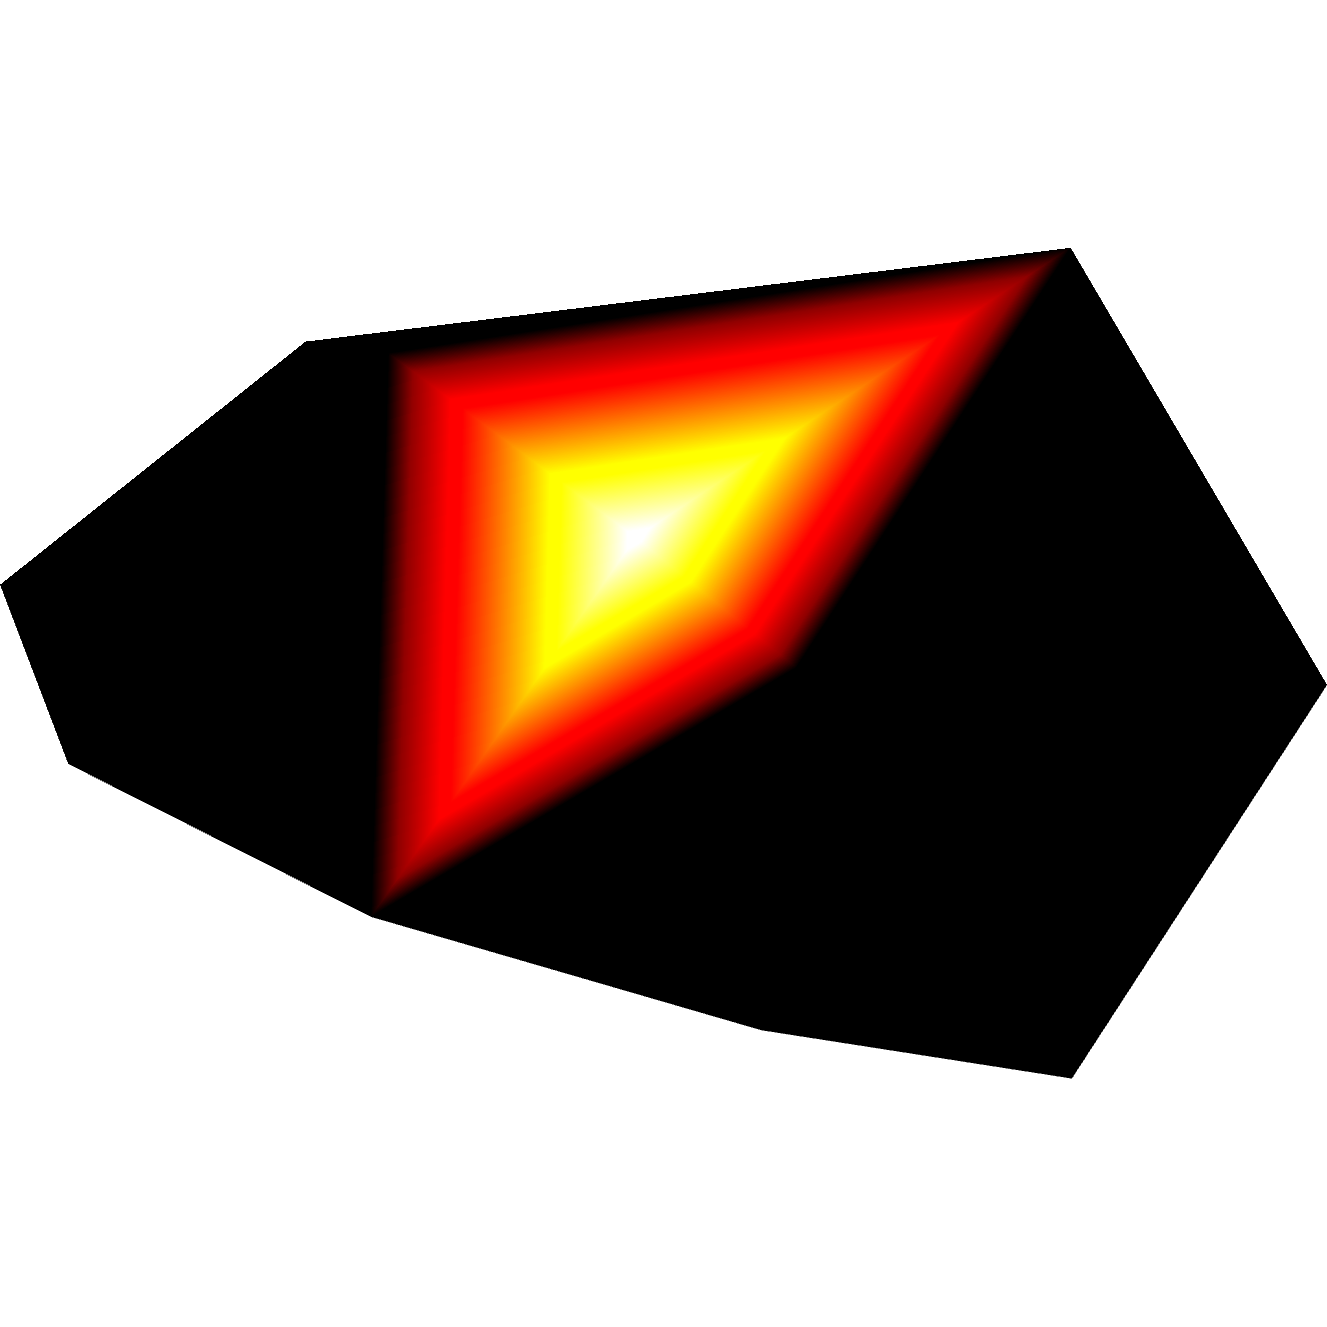
\includegraphics[width=1.0\linewidth,height=0.3\textheight,keepaspectratio]{data/synthetic_meshes/random_circle_tessellation_Dirac_delta_1_v11_f12_funcvals_0iter.png}
%		\caption{R.Circ v11\_f12 iter 2}\label{fig:rcirc.e}
%	\end{subfigure}
%	\begin{subfigure}[b]{0.48\linewidth}
%		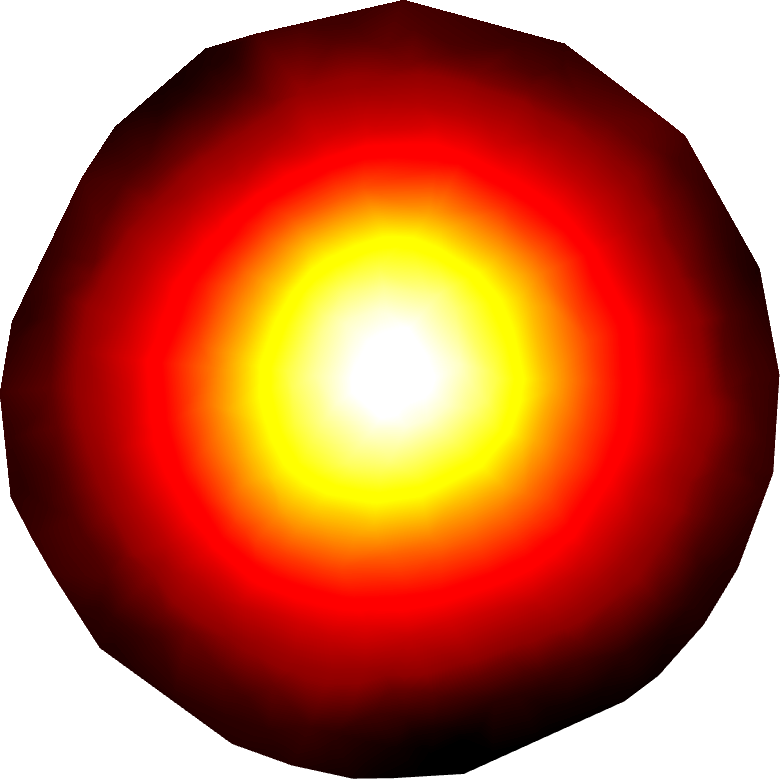
\includegraphics[width=1.0\linewidth,height=0.3\textheight,keepaspectratio]{data/synthetic_meshes/random_circle_tessellation_Dirac_delta_10_v641_f1252_funcvals_10000iter.png}
%		\caption{R.Circ v641\_f1252 iter 10,000}\label{fig:rcirc.f}
%	\end{subfigure}}
%	{\caption[Synthetic random vertices equally distributed per radius, Dirac delta function]{A synthetic circle filled with random vertices equaly distributed per radius, triangulated by Delauney method~\cite[p.~??]{todoCitation}, with a Dirac delta function applied: (a) v11\_f12 wireframe (b) v641\_f1252 wireframe (c) v11\_f12 colored by function value before filter (d) v641\_f1252 colored by function value before filter (e) v11\_f12 colored by function value after 2 iterations (f) v641\_f1252 colored by function value after 10,000 iterations.
%All using the colorramp "Hot (improved)"~\cite[p.~???]{Brewer2003}~\cite[p.~19]{Giga17}, visualized using GigaMesh~\cite{Mara10}, exported as png after disabling the background grid [f7], maximizing the window, disabling screenshot cropping, as well as rejecting tiled rendering, finally cropping to content in GIMP.
%}\label{fig:rcirc}}
%\end{figure}

\subsection{Mars Crater}
Mars dataset crater as a Digital Terrain Models (DTMs) Mention in Mara 3.6
Summary “Dali” inspired methodProcessing regular grids like Digital Terrain
Models (DTMs) will gain dramatic performance increases using the estimator,
while processing irregular grids with high curvatures will strongly benefit
from precise computation of the volume integral invariant.~\cite[p.~143]{Mara12}

\subsection{A Flat surface}
Flat surfaces have NOISE!
Figure~\ref{fig:ILATO}: ILATO\_1A\_SM2066-HE5-60\_070214\_merged\_GMO\_r1.00\_n4\_v256
\begin{figure}[ht]
\ffigbox
	{\begin{subfigure}[b]{0.48\linewidth}
		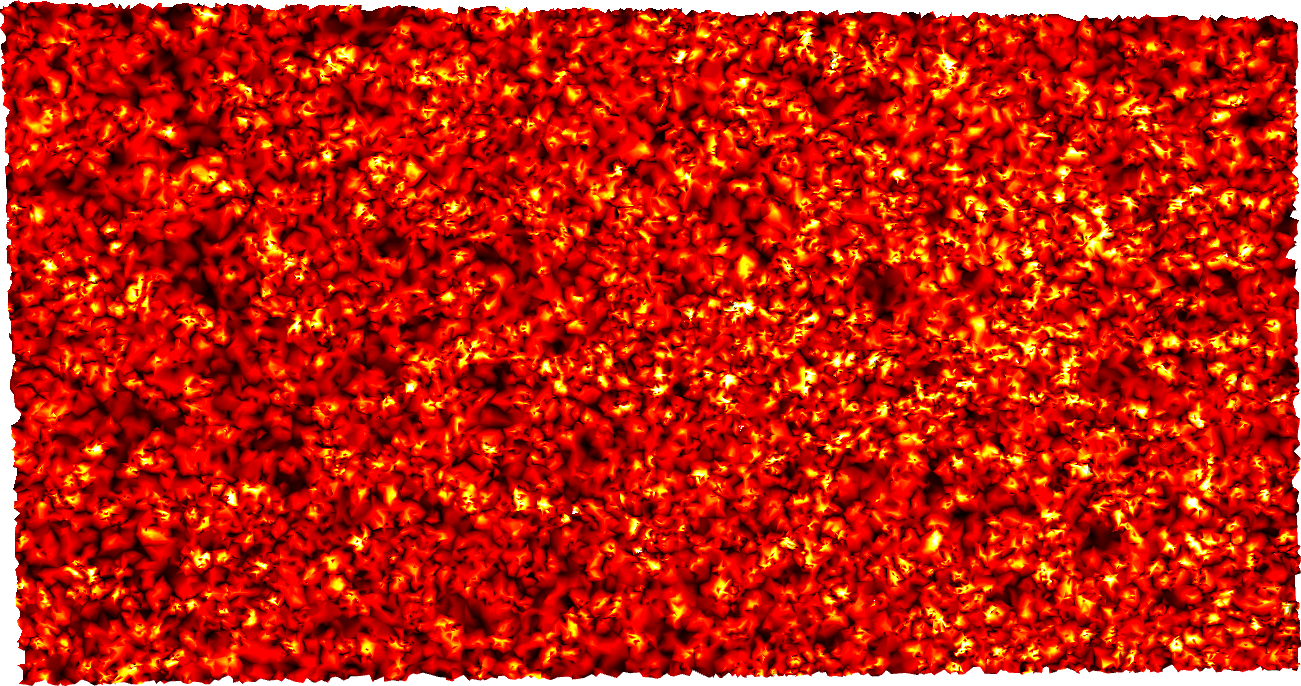
\includegraphics[width=1.0\linewidth,height=0.3\textheight,keepaspectratio]{data/acquired_meshes/ILATO_1A_SM2066-HE5-60_070214_merged_GMO_r1_n4_v256_funcvals_0iter.png}
		\caption{ILATO 0iter}\label{fig:ILATO.a}
	\end{subfigure}
	\begin{subfigure}[b]{0.48\linewidth}
		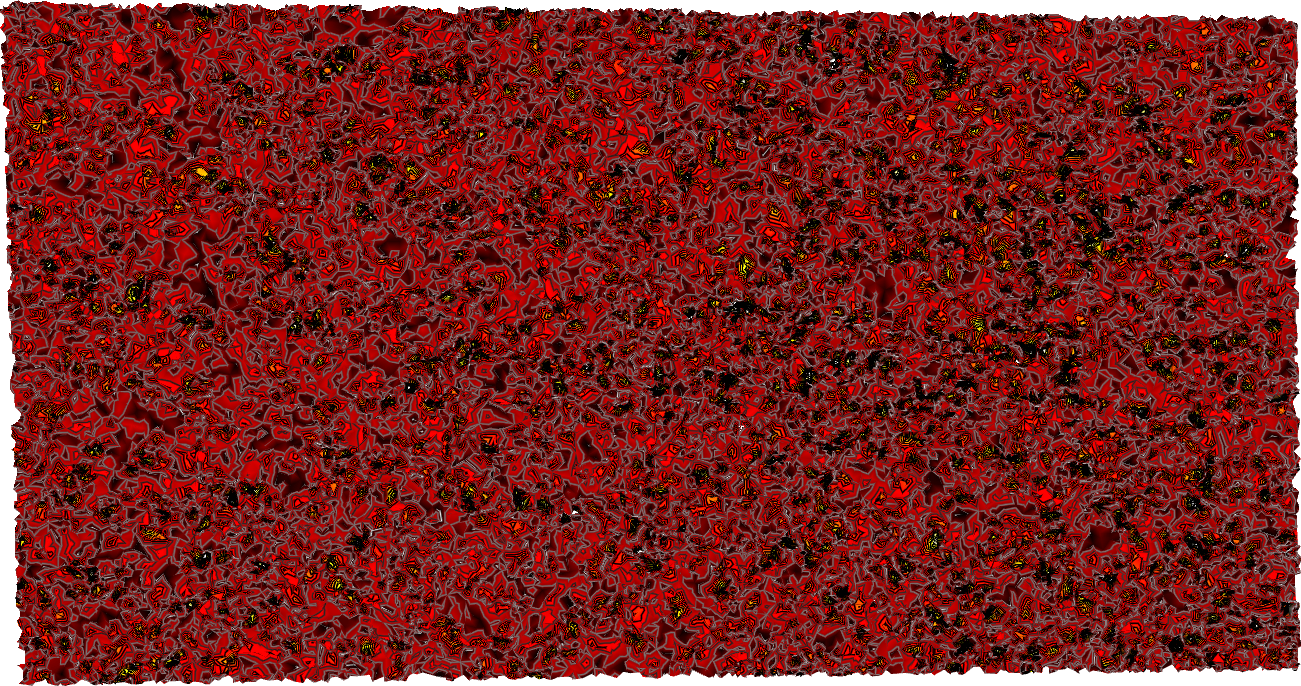
\includegraphics[width=1.0\linewidth,height=0.3\textheight,keepaspectratio]{data/acquired_meshes/ILATO_1A_SM2066-HE5-60_070214_merged_GMO_r1_n4_v256_funcvals_isolines_0iter.png}
		\caption{ILATO 0iter isolines}\label{fig:ILATO.b}
	\end{subfigure}

	\bigskip
	\begin{subfigure}[b]{0.48\linewidth}
		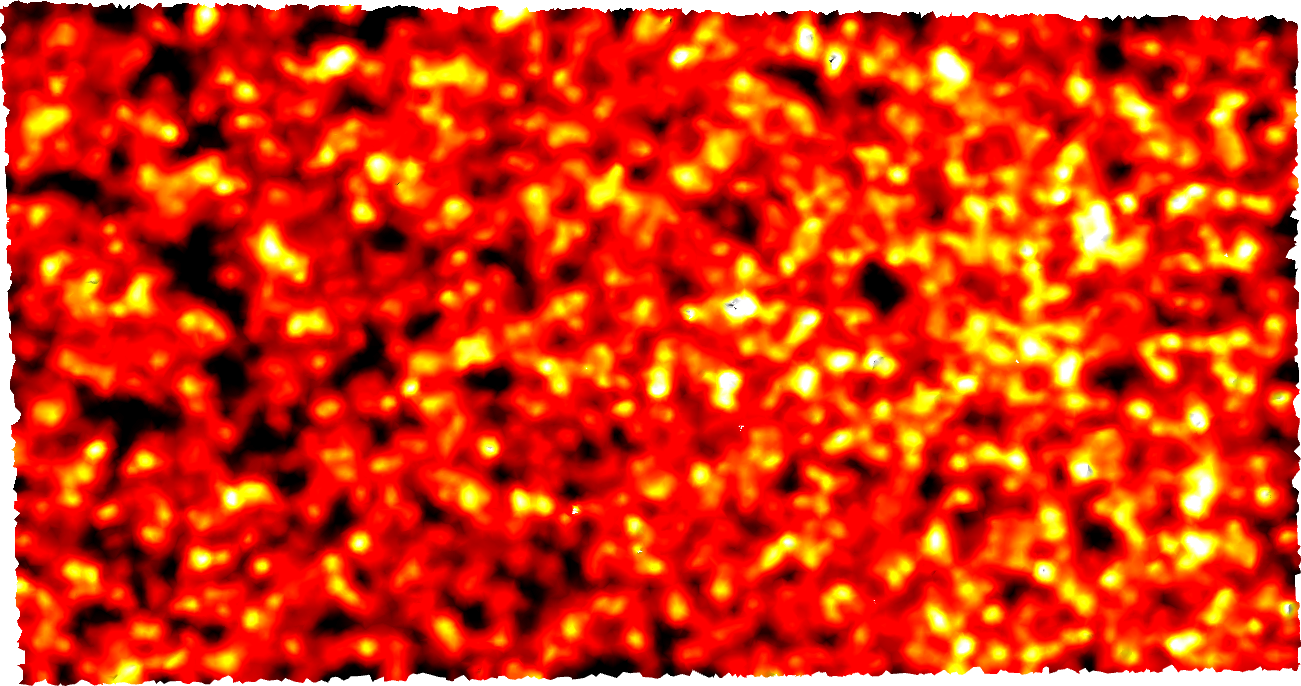
\includegraphics[width=1.0\linewidth,height=0.3\textheight,keepaspectratio]{data/acquired_meshes/ILATO_1A_SM2066-HE5-60_070214_merged_GMO_r1_n4_v256_funcvals_1000iter.png}
		\caption{ILATO 1000iter}\label{fig:ILATO.c}
	\end{subfigure}
	\begin{subfigure}[b]{0.48\linewidth}
		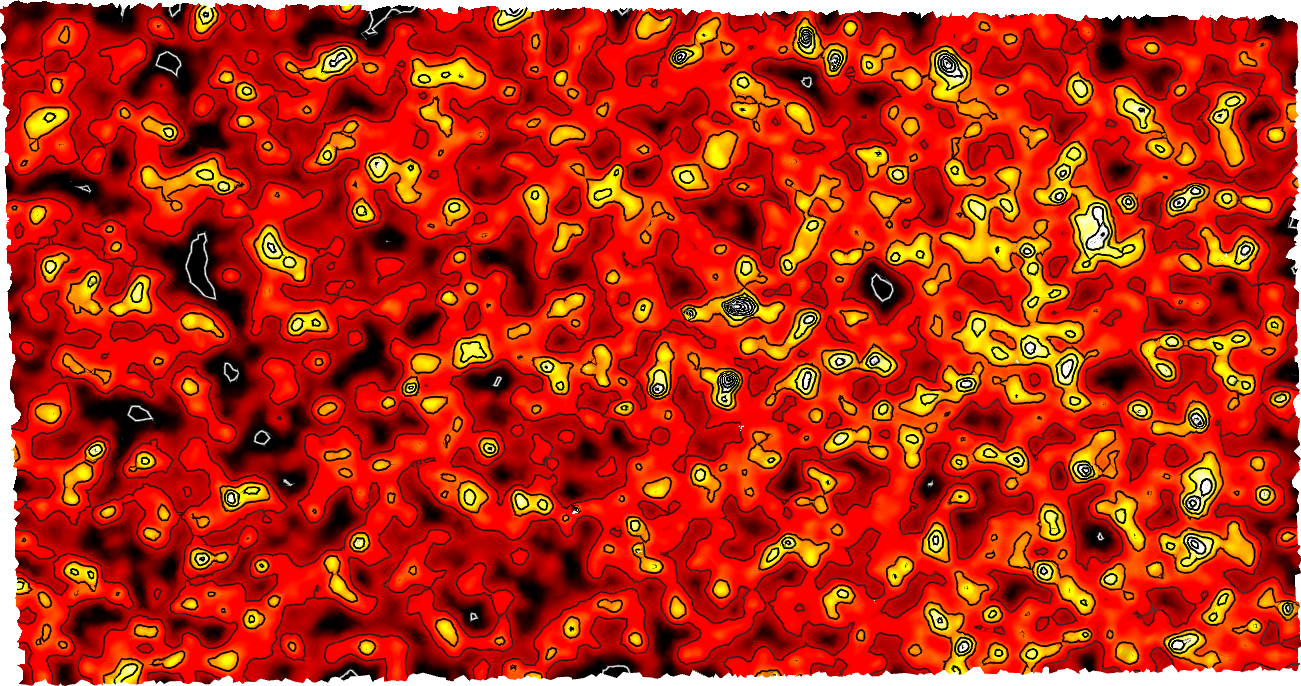
\includegraphics[width=1.0\linewidth,height=0.3\textheight,keepaspectratio]{data/acquired_meshes/ILATO_1A_SM2066-HE5-60_070214_merged_GMO_r1_n4_v256_funcvals_isolines_1000iter.png}
		\caption{ILATO 1000iter isolines}\label{fig:ILATO.d}
	\end{subfigure}

	\bigskip
	\begin{subfigure}[b]{0.48\linewidth}
		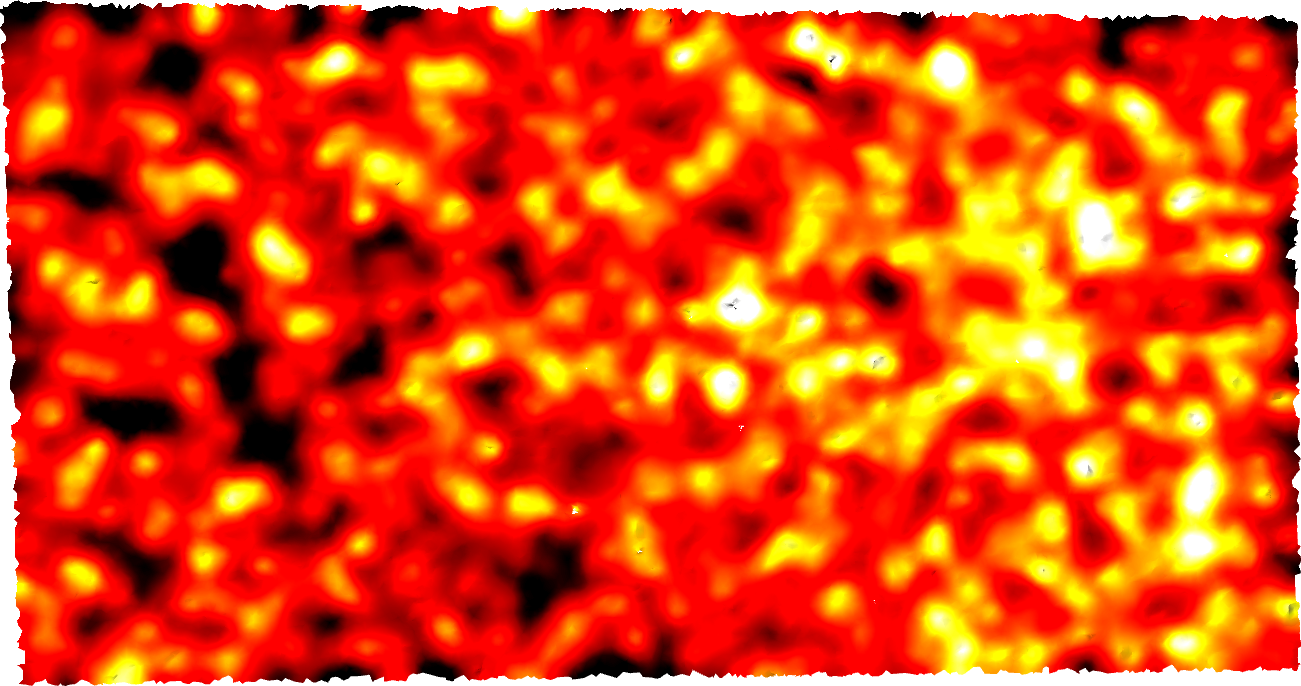
\includegraphics[width=1.0\linewidth,height=0.3\textheight,keepaspectratio]{data/acquired_meshes/ILATO_1A_SM2066-HE5-60_070214_merged_GMO_r1_n4_v256_funcvals_3000iter.png}
		\caption{ILATO 3000iter}\label{fig:ILATO.e}
	\end{subfigure}
	\begin{subfigure}[b]{0.48\linewidth}
		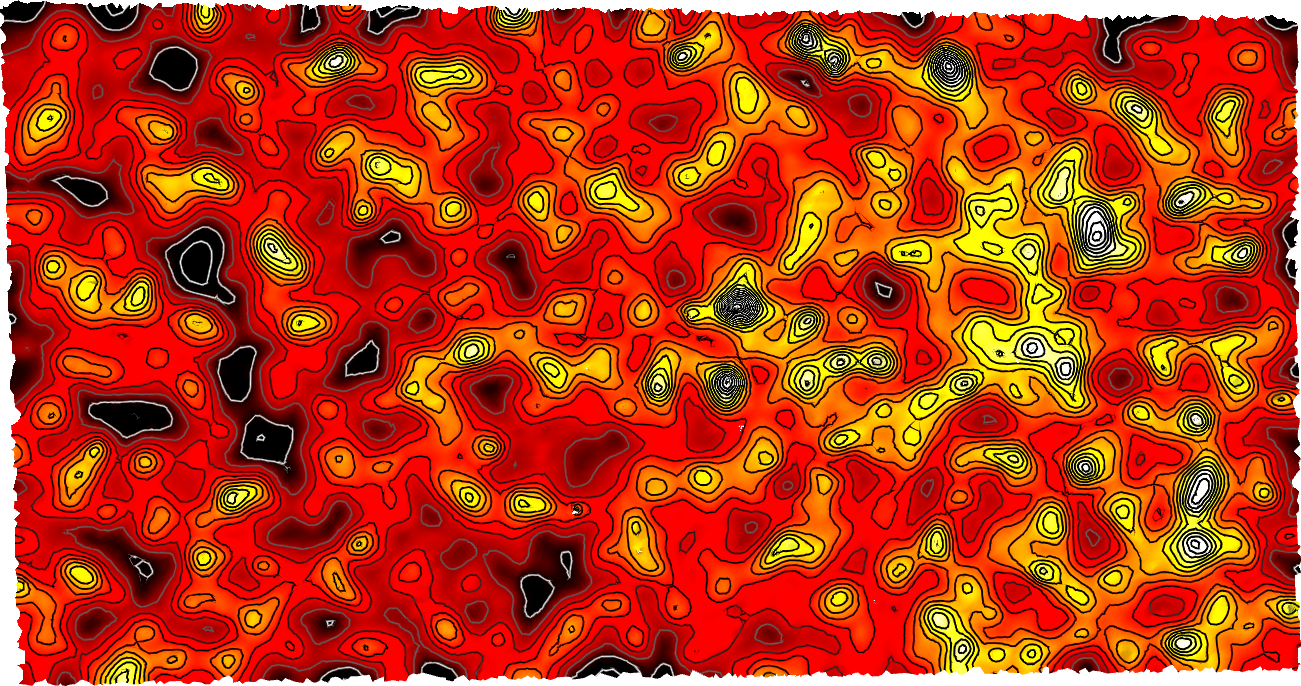
\includegraphics[width=1.0\linewidth,height=0.3\textheight,keepaspectratio]{data/acquired_meshes/ILATO_1A_SM2066-HE5-60_070214_merged_GMO_r1_n4_v256_funcvals_isolines_3000iter.png}
		\caption{ILATO 3000iter isolines}\label{fig:ILATO.f}
	\end{subfigure}}
	{\caption[ILATO]{ILATO\_1A\ldots}\label{fig:ILATO}}
\end{figure}

\subsection{Stanford Bunny}
Figure~\ref{fig:bun}: http://graphics.stanford.edu/data/3Dscanrep/ (Stanford Bunny)
\begin{figure}[ht]
\ffigbox
	{\begin{subfigure}[b]{0.48\linewidth}
		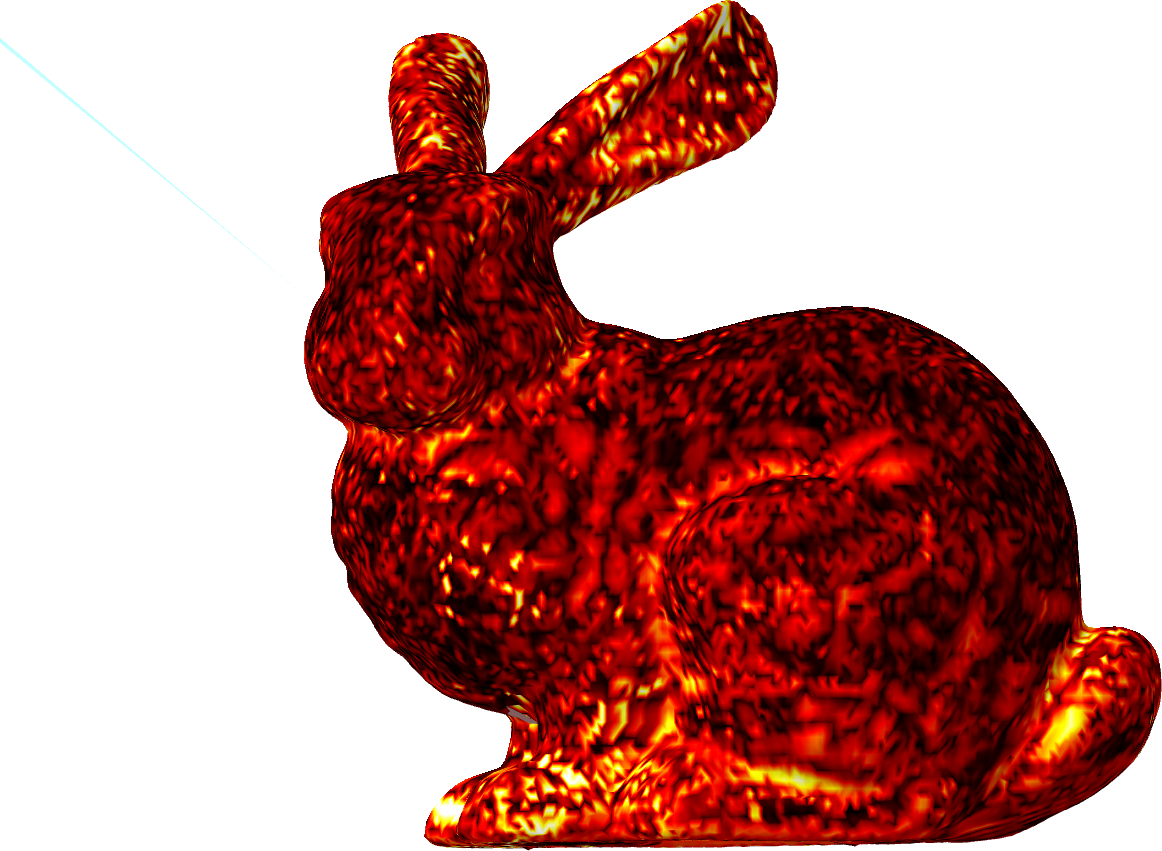
\includegraphics[width=1.0\linewidth,height=0.3\textheight,keepaspectratio]{data/acquired_meshes/bun_zipper_edited_r1_n4_v256_funcvals_0iter.png}
		\caption{Stanford Bunny 0iter}\label{fig:bun.a}
	\end{subfigure}
	\begin{subfigure}[b]{0.48\linewidth}
		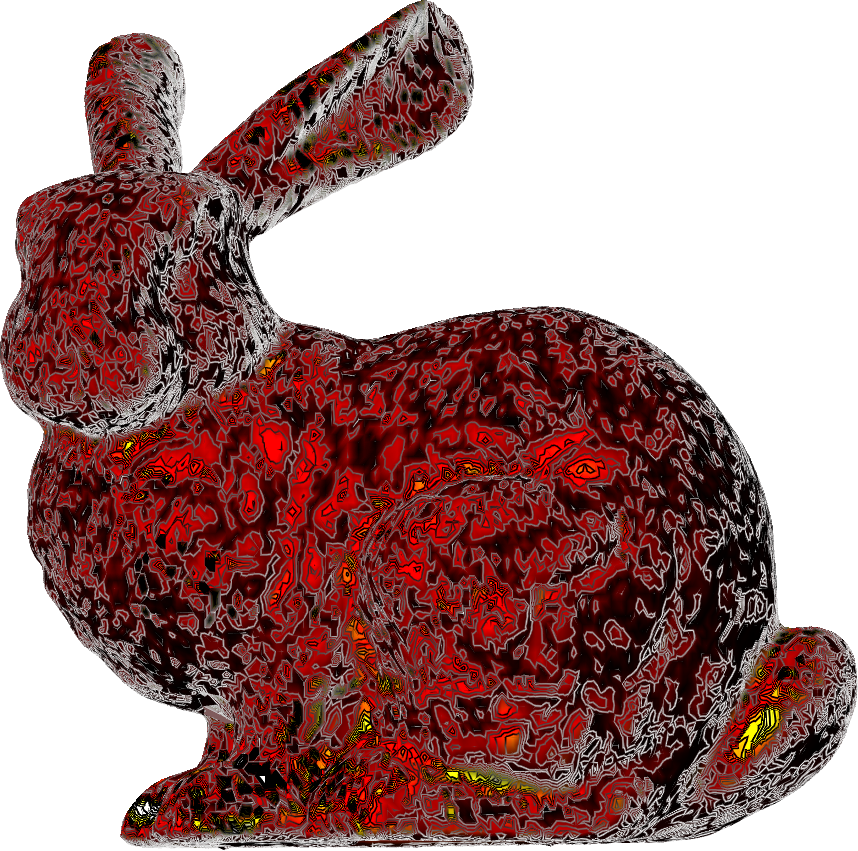
\includegraphics[width=1.0\linewidth,height=0.3\textheight,keepaspectratio]{data/acquired_meshes/bun_zipper_edited_r1_n4_v256_funcvals_isolines_0iter.png}
		\caption{Stanford Bunny 0iter isolines}\label{fig:bun.b}
	\end{subfigure}

	\bigskip
	\begin{subfigure}[b]{0.48\linewidth}
		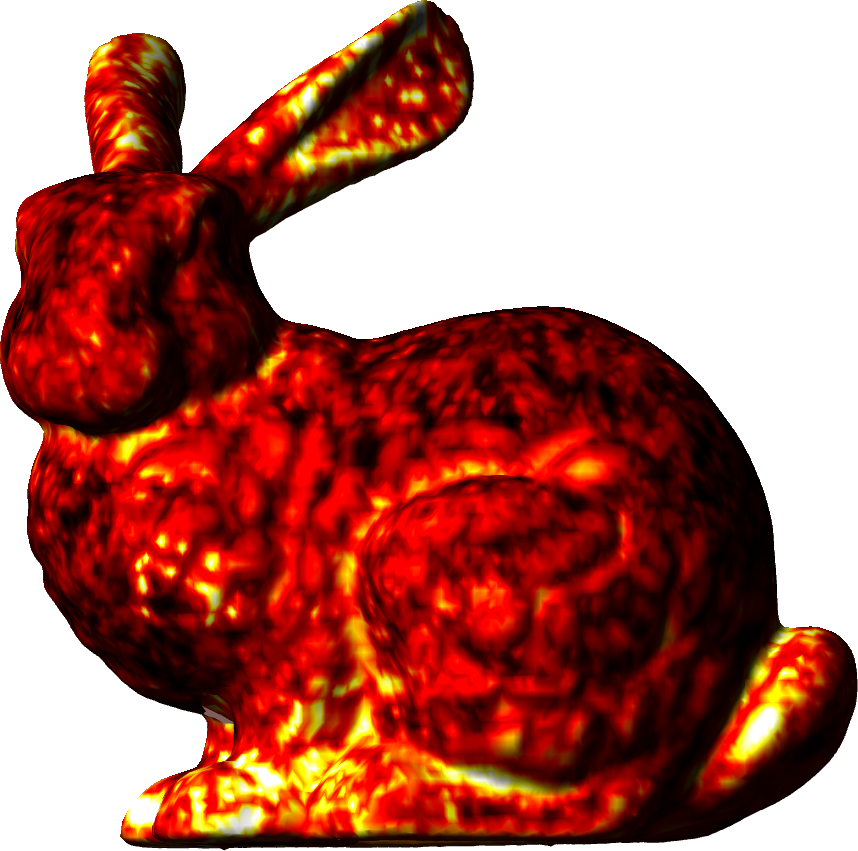
\includegraphics[width=1.0\linewidth,height=0.3\textheight,keepaspectratio]{data/acquired_meshes/bun_zipper_edited_r1_n4_v256_funcvals_10iter.png}
		\caption{Stanford Bunny 10iter}\label{fig:bun.c}
	\end{subfigure}
	\begin{subfigure}[b]{0.48\linewidth}
		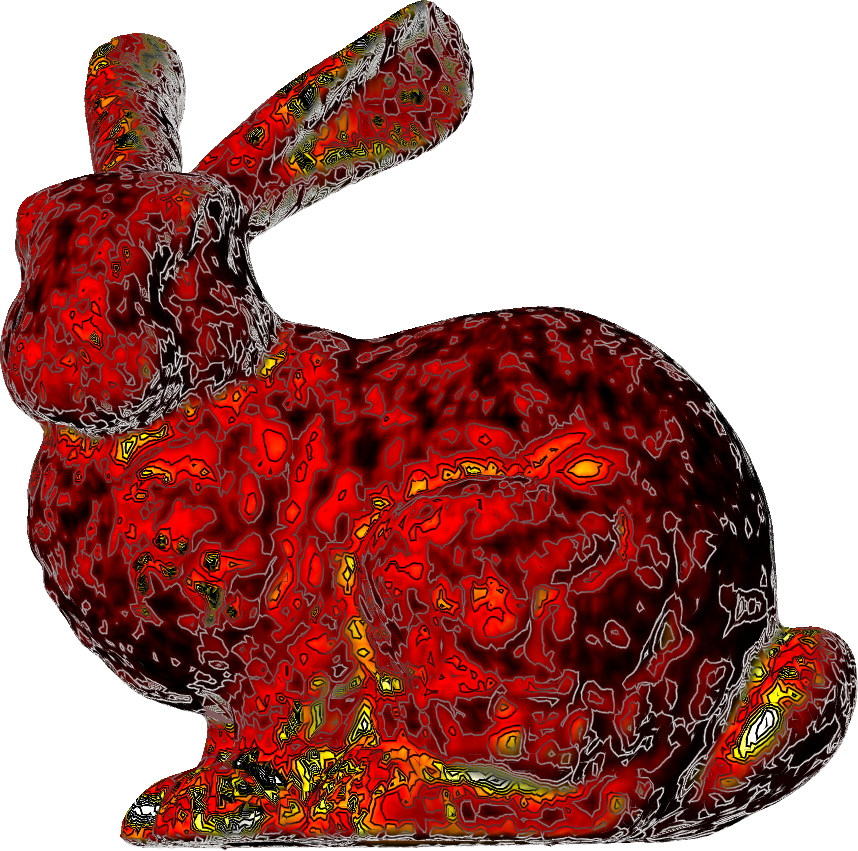
\includegraphics[width=1.0\linewidth,height=0.3\textheight,keepaspectratio]{data/acquired_meshes/bun_zipper_edited_r1_n4_v256_funcvals_isolines_10iter.png}
		\caption{Stanford Bunny 10iter isolines}\label{fig:bun.d}
	\end{subfigure}

	\bigskip
	\begin{subfigure}[b]{0.48\linewidth}
		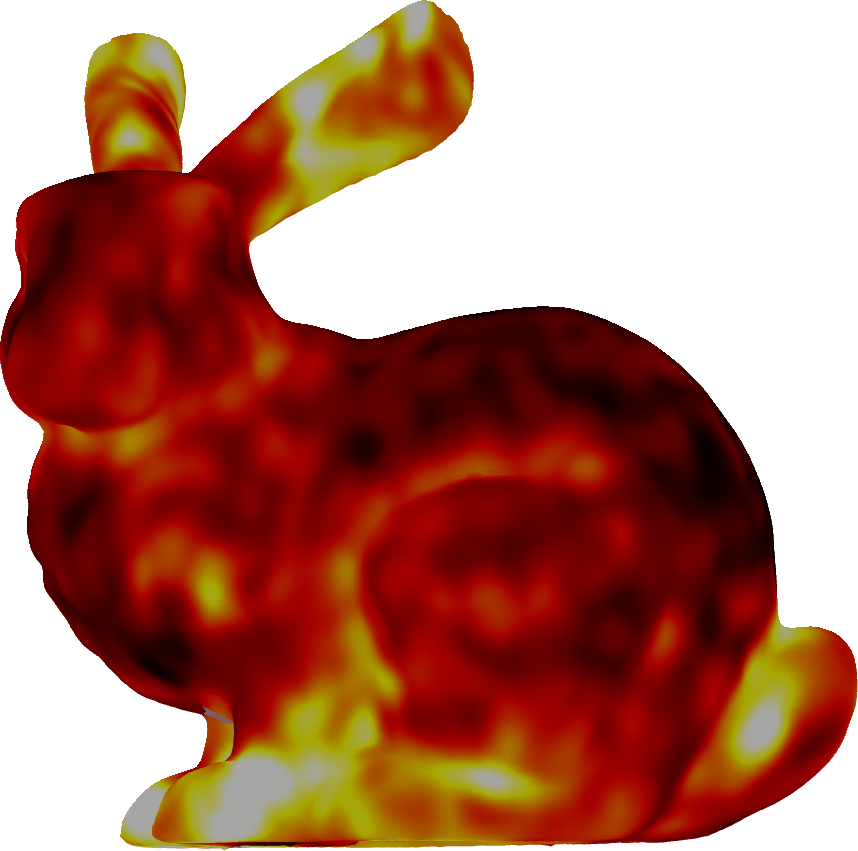
\includegraphics[width=1.0\linewidth,height=0.3\textheight,keepaspectratio]{data/acquired_meshes/bun_zipper_edited_r1_n4_v256_funcvals_100iter.png}
		\caption{Stanford Bunny Wireframe}\label{fig:bun.e}
	\end{subfigure}
	\begin{subfigure}[b]{0.48\linewidth}
		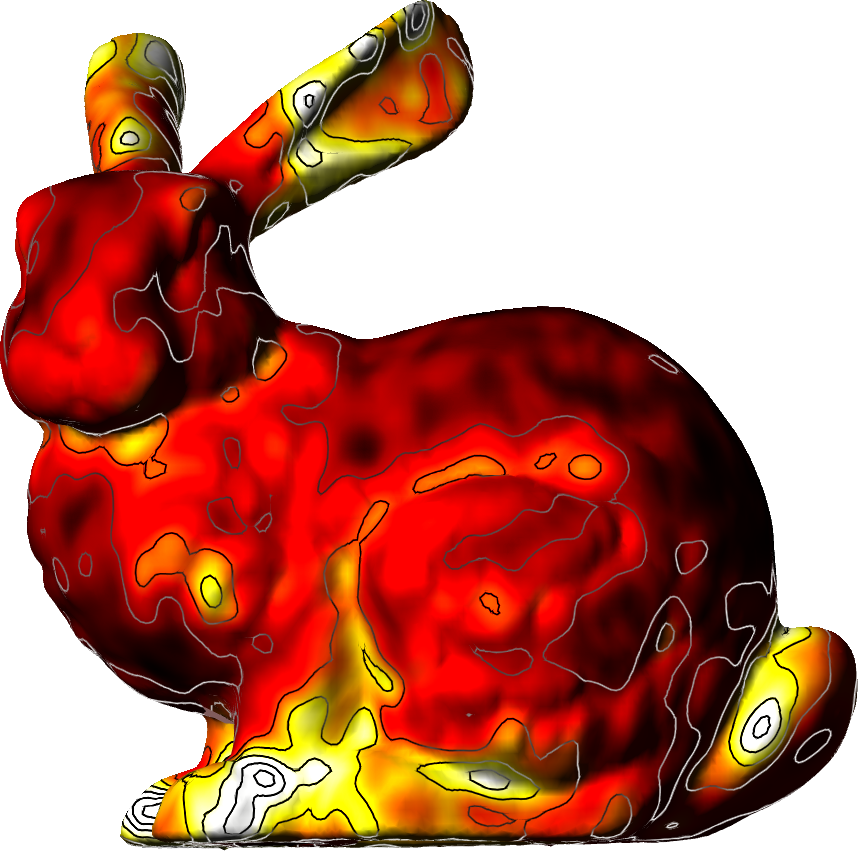
\includegraphics[width=1.0\linewidth,height=0.3\textheight,keepaspectratio]{data/acquired_meshes/bun_zipper_edited_r1_n4_v256_funcvals_isolines_100iter.png}
		\caption{Stanford Bunny 100iter isolines}\label{fig:bun.f}
	\end{subfigure}}
	{\caption[Stanford Bunny]{Stanford Bunny\ldots}\label{fig:bun}}
\end{figure}



\section{Evaluation}
\subsection{Compute Times}

Figure~\ref{fig:computeTimesLP} shows how compute times increase linearly with both mesh size and number of iterations in a very predictable way when total compute time is at least 0.1 seconds, and less predictable for shorter periods do to the nature of thread optimization at the processor level and variable memory read times.\todoResearch{add formula for timing (or at least ref to it) here.}\todoResearch{process time noise at very fast speeds}
\begin{figure}[ht]
	\centering
	\includegraphics[width=1.0\linewidth,height=1.0\textheight,keepaspectratio]{figures/computeTimesLinespoints.png}
	\RawCaption{\caption[Compute Times - Linespoints]{Compute Times of Applying
		the	One-Ring Filter for Selected Numbers of Iterations onto Acquired and
		Synthetic 3D Meshes of Varying Sizes}
		\label{fig:computeTimesLP}}
\end{figure}

Figure~\ref{fig:computeTimesS} shows how compute times increase with both meshsize and number of iterations.\todoCitation{wikipedia Euler characteristic Polyhedra}
\begin{figure}[ht]
	\centering
	\includegraphics[width=1.0\linewidth,height=1.0\textheight,keepaspectratio]{figures/computeTimesScatter.png}
	\RawCaption{\caption[Compute Times - Scatter]{Compute Times for Different
		Hardware Configurations by increaseing Mesh Size and Filter Iterations}
		\label{fig:computeTimesS}}
\end{figure}

\begin{figure}[ht]
	\centering
	\includegraphics[width=1.0\linewidth,height=1.0\textheight,keepaspectratio]{figures/numFacesByVerticesGoTo2.png}
	\RawCaption{\caption[Ratio of Faces / Vertices]{Ratio of Faces to Vertices by
		Increasing Vertex Count}
		\label{fig:ratioFacesVertices}}
\end{figure}





\section{Summary}
Lorem ipsum dolor sit amet, consectetur adipiscing elit. Morbi tincidunt eget
ipsum eu iaculis. Cras vel sem eu velit eleifend porta vel sit amet massa. Etiam
a posuere nunc. Aenean aliquam viverra dapibus. Aliquam ac eros a purus feugiat
rhoncus. Donec faucibus ut nibh ut cursus. Aliquam erat volutpat. Proin efficitur
nulla sit amet iaculis condimentum. Cras placerat leo vitae venenatis feugiat. In
hac habitasse platea dictumst. Orci varius natoque penatibus et magnis dis
parturient montes, nascetur ridiculus mus. In aliquet sagittis dui eu pulvinar.
Morbi a arcu eu dolor sagittis varius. Aliquam dignissim tortor sed tortor
suscipit, eget imperdiet mauris convallis.

\chapter{Distribution}
CLI - commandline interface only
Focus on theoretical work 
And specifics regarding CUDA considerations regarding its limitations
MAYBE 1 page
Dependencies
Linux vs Windows



\section{Standalone Precompiled Binary}
CLI - commandline interface only



\section{Integration with Legacy Code (GigaMesh)}
CLI - commandline interface or GUI - graphical user interface are possible
\begin{enumerate}
\item Make GigaMesh CUDA aware
	\begin{enumerate}
	\item Update Makefile to include nvcc compiler and new source files
	\item second item
	\end{enumerate}
\item second item
\end{enumerate}
Before CUDA 5.0, if a programmer wanted to call particle::advance() from a CUDA 
kernel launched in main.cpp, the compiler required the main.cpp compilation unit 
to include the implementation of particle::advance() as well any subroutines it 
calls (v3::normalize() and v3::scramble() in this case). In complex C++ 
applications, the call chain may go deeper than the two-levels that our example 
illustrates. Without device object linking, the developer may need to deviate 
from the conventional application structure to accommodate this compiler 
requirement. Such changes are difficult for existing applications in which 
changing the structure is invasive and/or undesirable.~\cite{Cuda14}
In order to use the full functionality of GigaMesh a batch program has to be run 
for generating feature vectors. These vectors contain additional information per 
vertex concerning surface and volume of a set of spheres intersecting the mesh. 
See [MKJB10] for more background information on the Multi Scale Integral 
Invariant (MSII) filtering technique. This operation is rather time consuming 
(it takes hours or even days of computing time) and therefore better runs 
without graphical user interface. Although generating feature vectors is quite 
robust against solo vertices, singularities, non-manifolds and holes, you should 
first clean up your mesh data to get a proper result. So switch to the advanced 
task of polishing your mesh in section 4.1 and return to this section when you 
have got a cleaned mesh. If you do not want to manipulate your mesh you may 
continue directly. Open a terminal and type and change to the mesh-folder by 
typing cd GigaMesh/mesh (note that GigaMesh stands for the GigaMesh installation 
folder). Then start the program nohup ./meshgeneratorfeaturevectors25d\_threads 
-f [-r 2] \& and use nohup at the beginning of the command and \& at the end to 
ensure that the job runs in the background. This is because this step can take 
several hours and you do not want to block the terminal.~\cite[p.~19]{Giga17}



\section{Summary}
Lorem ipsum dolor sit amet, consectetur adipiscing elit. Morbi tincidunt eget 
ipsum eu iaculis. Cras vel sem eu velit eleifend porta vel sit amet massa. Etiam 
a posuere nunc. Aenean aliquam viverra dapibus. Aliquam ac eros a purus feugiat 
rhoncus. Donec faucibus ut nibh ut cursus. Aliquam erat volutpat. Proin efficitur 
nulla sit amet iaculis condimentum. Cras placerat leo vitae venenatis feugiat. In 
hac habitasse platea dictumst. Orci varius natoque penatibus et magnis dis 
parturient montes, nascetur ridiculus mus. In aliquet sagittis dui eu pulvinar. 
Morbi a arcu eu dolor sagittis varius. Aliquam dignissim tortor sed tortor 
suscipit, eget imperdiet mauris convallis.

\chapter{Conclusions}
\section{Summary}
Lorem ipsum dolor sit amet, consectetur adipiscing elit. Morbi tincidunt eget 
ipsum eu iaculis. Cras vel sem eu velit eleifend porta vel sit amet massa. Etiam 
a posuere nunc. Aenean aliquam viverra dapibus. Aliquam ac eros a purus feugiat 
rhoncus. Donec faucibus ut nibh ut cursus. Aliquam erat volutpat. Proin efficitur 
nulla sit amet iaculis condimentum. Cras placerat leo vitae venenatis feugiat. In 
hac habitasse platea dictumst. Orci varius natoque penatibus et magnis dis 
parturient montes, nascetur ridiculus mus. In aliquet sagittis dui eu pulvinar. 
Morbi a arcu eu dolor sagittis varius. Aliquam dignissim tortor sed tortor 
suscipit, eget imperdiet mauris convallis.

Aliquam in justo ut est eleifend facilisis vitae nec mi. Suspendisse pellentesque, 
ligula ut mattis volutpat, ex risus scelerisque ligula, at ornare arcu augue ut r
isus. Integer non pellentesque quam, quis laoreet nisi. Donec aliquam leo mi, vel 
consectetur magna vestibulum eu. Ut quis efficitur metus. Donec consequat mi nec 
pellentesque rhoncus. Phasellus sit amet laoreet quam. Quisque dictum ex non elit 
aliquet lobortis. Quisque molestie egestas dolor vel interdum. In fermentum sit 
amet mi non venenatis. In ut tempus arcu.

Donec arcu eros, vestibulum maximus volutpat nec, euismod a purus. Nullam bibendum 
eros posuere sem sollicitudin, vitae porttitor ex scelerisque. Sed nisi felis, 
consectetur sed lacinia vitae, egestas non nibh. Curabitur a ex sed neque lacinia 
tempor sit amet consectetur ipsum. Sed et eros dictum, dictum magna lacinia, 
elementum lacus. Praesent enim tortor, semper ut egestas at, faucibus quis metus. 
Aliquam mattis, lorem et ultrices mattis, erat neque bibendum est, nec condimentum 
ex tellus sit amet diam. In sollicitudin placerat diam, lobortis efficitur leo. 
Integer id erat tellus. Ut quis odio velit. Nulla facilisi. Donec mollis 
scelerisque lobortis. Nam eu felis sed purus feugiat semper ac ac ante. Maecenas 
faucibus odio diam, id tristique orci placerat sed. Ut vel ex metus. Maecenas 
tempus velit gravida nulla viverra, in suscipit enim mattis.


\section{Future Work}
What they are and why I did not.
OpenMP
PThreads
(already impl’d in GigaMesh)
OpenCL
Pipelining memory reads/calculations exploit more concurrency
Thread indexing 3D vs 1D
Determine is using $\Dm$ vs $\bar{\Dm}$ has any effect, especially on one-ring neighborhood with a relatively large $\Dm$ on mesh with a very small $\bar{\Dm}$ 

%
\appendix
\chapter{Maybe some appendix please?}
Lorem ipsum dolor sit amet, consectetur adipiscing elit. Morbi tincidunt eget 
ipsum eu iaculis. Cras vel sem eu velit eleifend porta vel sit amet massa. Etiam 
a posuere nunc. Aenean aliquam viverra dapibus. Aliquam ac eros a purus feugiat 
rhoncus. Donec faucibus ut nibh ut cursus. Aliquam erat volutpat. Proin efficitur 
nulla sit amet iaculis condimentum. Cras placerat leo vitae venenatis feugiat. In 
hac habitasse platea dictumst. Orci varius natoque penatibus et magnis dis 
parturient montes, nascetur ridiculus mus. In aliquet sagittis dui eu pulvinar. 
Morbi a arcu eu dolor sagittis varius. Aliquam dignissim tortor sed tortor 
suscipit, eget imperdiet mauris convallis.

Aliquam in justo ut est eleifend facilisis vitae nec mi. Suspendisse pellentesque, 
ligula ut mattis volutpat, ex risus scelerisque ligula, at ornare arcu augue ut r
isus. Integer non pellentesque quam, quis laoreet nisi. Donec aliquam leo mi, vel 
consectetur magna vestibulum eu. Ut quis efficitur metus. Donec consequat mi nec 
pellentesque rhoncus. Phasellus sit amet laoreet quam. Quisque dictum ex non elit 
aliquet lobortis. Quisque molestie egestas dolor vel interdum. In fermentum sit 
amet mi non venenatis. In ut tempus arcu.

Donec arcu eros, vestibulum maximus volutpat nec, euismod a purus. Nullam bibendum 
eros posuere sem sollicitudin, vitae porttitor ex scelerisque. Sed nisi felis, 
consectetur sed lacinia vitae, egestas non nibh. Curabitur a ex sed neque lacinia 
tempor sit amet consectetur ipsum. Sed et eros dictum, dictum magna lacinia, 
elementum lacus. Praesent enim tortor, semper ut egestas at, faucibus quis metus. 
Aliquam mattis, lorem et ultrices mattis, erat neque bibendum est, nec condimentum 
ex tellus sit amet diam. In sollicitudin placerat diam, lobortis efficitur leo. 
Integer id erat tellus. Ut quis odio velit. Nulla facilisi. Donec mollis 
scelerisque lobortis. Nam eu felis sed purus feugiat semper ac ac ante. Maecenas 
faucibus odio diam, id tristique orci placerat sed. Ut vel ex metus. Maecenas 
tempus velit gravida nulla viverra, in suscipit enim mattis.

\chapter{Just another appendix.}
Lorem ipsum dolor sit amet, consectetur adipiscing elit. Morbi tincidunt eget 
ipsum eu iaculis. Cras vel sem eu velit eleifend porta vel sit amet massa. Etiam 
a posuere nunc. Aenean aliquam viverra dapibus. Aliquam ac eros a purus feugiat 
rhoncus. Donec faucibus ut nibh ut cursus. Aliquam erat volutpat. Proin efficitur 
nulla sit amet iaculis condimentum. Cras placerat leo vitae venenatis feugiat. In 
hac habitasse platea dictumst. Orci varius natoque penatibus et magnis dis 
parturient montes, nascetur ridiculus mus. In aliquet sagittis dui eu pulvinar. 
Morbi a arcu eu dolor sagittis varius. Aliquam dignissim tortor sed tortor 
suscipit, eget imperdiet mauris convallis.

Aliquam in justo ut est eleifend facilisis vitae nec mi. Suspendisse pellentesque, 
ligula ut mattis volutpat, ex risus scelerisque ligula, at ornare arcu augue ut r
isus. Integer non pellentesque quam, quis laoreet nisi. Donec aliquam leo mi, vel 
consectetur magna vestibulum eu. Ut quis efficitur metus. Donec consequat mi nec 
pellentesque rhoncus. Phasellus sit amet laoreet quam. Quisque dictum ex non elit 
aliquet lobortis. Quisque molestie egestas dolor vel interdum. In fermentum sit 
amet mi non venenatis. In ut tempus arcu.

Donec arcu eros, vestibulum maximus volutpat nec, euismod a purus. Nullam bibendum 
eros posuere sem sollicitudin, vitae porttitor ex scelerisque. Sed nisi felis, 
consectetur sed lacinia vitae, egestas non nibh. Curabitur a ex sed neque lacinia 
tempor sit amet consectetur ipsum. Sed et eros dictum, dictum magna lacinia, 
elementum lacus. Praesent enim tortor, semper ut egestas at, faucibus quis metus. 
Aliquam mattis, lorem et ultrices mattis, erat neque bibendum est, nec condimentum 
ex tellus sit amet diam. In sollicitudin placerat diam, lobortis efficitur leo. 
Integer id erat tellus. Ut quis odio velit. Nulla facilisi. Donec mollis 
scelerisque lobortis. Nam eu felis sed purus feugiat semper ac ac ante. Maecenas 
faucibus odio diam, id tristique orci placerat sed. Ut vel ex metus. Maecenas 
tempus velit gravida nulla viverra, in suscipit enim mattis.

%
\backmatter
\printindex
\bibliography{thesis}{}
\bibliographystyle{plain}
\todoRemove{remove todoCitation from bibliography}
\todoStyle{should bibliographystyle be plain?}

\end{document}

